\documentclass[12pt,a4paper,twoside,openright]{report}

\usepackage[table,xcdraw]{xcolor}
\usepackage{array}
\usepackage{colortbl}

\usepackage[pdftex]{graphicx} % Biblioteca para uso de figuras
\usepackage{color}

\usepackage[brazil]{babel} % Biblioteca para uso da l�ngua portuguesa
\usepackage[T1]{fontenc} % Biblioteca para uso da acentua��o de entrada
\usepackage[latin1]{inputenc} % Biblioteca para uso da acentua��o de sa�da

\usepackage{indentfirst}

\usepackage{caption}

\usepackage{subcaption}

\usepackage{cleveref}

\usepackage[export]{adjustbox}





\usepackage{amsthm,amsfonts,amsmath,amssymb}  % Biblioteca para uso de comandos matem�ticos
\usepackage{pslatex}
\usepackage{pstricks,pst-node,color,pst-gantt,pst-coil}
\usepackage{scalefnt}
\usepackage{float} %Permite colocar "\begin{figure}[H]" e colocar imagem exatamente onde desejar
\usepackage[hyphens]{url} % Para Aceitar URL nas referencias
\usepackage{pdfpages}

\usepackage{eurosym} %Pacote para possibilitar o uso do s�mbolo de euro "\euro"

\usepackage{listings} % para importa��o de c�digos fonte 

\usepackage{setspace}

\usepackage{comment}

%\usepackage[margin=2.7cm]{geometry}
\renewcommand{\baselinestretch}{1.5}

\setlength{\parskip}{0em}

% Pacote para configurar cabe�alho e rodape
\usepackage{fancyhdr}
\pagestyle{empty}
\fancyhf{} % clear all header and footer fields

\fancypagestyle{plain}{\pagestyle{fancy}}
\renewcommand{\headrulewidth}{0pt}
\renewcommand{\footrulewidth}{0pt}

%Pacote para organizar apendices 
\usepackage[titletoc]{appendix}

\usepackage{rotating}

%%%%%%%%%%%%%%%%%%%%%%%%%%%%%%%%%%%%%% CONFIGURA��ES DE ANEXOS %%%%%%%%%%%%%%%%%%%%%%%%%%%%%%%%%%%%%%

\newcommand{\annexname}{Anexo}
\makeatletter
\newcommand\annex{\par
  \setcounter{chapter}{0}%
  \setcounter{section}{0}%
  \gdef\@chapapp{\annexname}%
  \gdef\thechapter{\@Roman\c@chapter}}
\makeatother

\newenvironment{poliabstract}[1]
  {\renewcommand{\abstractname}{#1}\begin{abstract}}
  {\end{abstract}}

%%%%%%%%%%%%%

\usepackage{mathptmx}
\usepackage{helvet}
\renewcommand{\familydefault}{\sfdefault}
	
 %\usepackage[T1]{fontenc}
 %\usepackage[scaled]{uarial}
 %\renewcommand*\familydefault{\sfdefault}	
	
	%\pdfmapfile{=<name>.map}
	
\renewcommand{\baselinestretch}{1.5} 	

\setlength\parindent{1cm}

\let\locdimen\newdimen

\usepackage{etex}

\usepackage{bytefield}

\usepackage{titlesec}
\titlespacing*{\chapter}{0pt}{-0.5cm}{20pt}

\titleformat{\chapter}{\fontsize{16pt}{5mm}\selectfont\bfseries}{\hspace{1cm}\thechapter}{1em}{}
\titleformat{\section}{\fontsize{13.5pt}{5mm}\selectfont\bfseries}{\hspace{1cm}\thesection}{1em}{}
\titleformat{\subsection}{\fontsize{13.5pt}{5mm}\selectfont\bfseries}{\hspace{1cm}\thesubsection}{1em}{}

\usepackage[top=3cm, bottom=2cm, left=3cm, right=2cm]{geometry}


%\usepackage{titlesec}
%\titleformat{\section}[display]
%{\hspace{1cm}\fontsize{12pt}{5mm}\selectfont\bfseries}{\thesection}{1em}{}

%\usepackage{titlesec}
%\titleformat{\subsection}
%{\hspace{1cm}\fontsize{12pt}{5mm}\selectfont\bfseries}{\thesubsection}{1em}{}

%%%%%%%%%%%%%%%%%%%%%%%%%%%%%%%%%%%%%% CONFIGURA��ES DE P�GINA %%%%%%%%%%%%%%%%%%%%%%%%%%%%%%%%%%%%%%
%\topmargin -2.1cm
%\oddsidemargin 0.5cm 
%\evensidemargin 0.5cm 
%\textwidth 15cm
%\textheight 25.1cm

%\usepackage{hyperref}


%%%%%%%%%%%%%%%%%%%%%%%%%%%%%%%%%%%%%%%% IN�CIO DO DOCUMENTO %%%%%%%%%%%%%%%%%%%%%%%%%%%%%%%%%%%%%%%%
\begin{document}

%%%%%%%%%%%%%%%%%%%%%%%%%%%%%%%%%%%%%%  INCLUDES %%%%%%%%%%%%%%%%%%%%%%%%%%%%%%%%%%%%%%

%%%%%%%%%%%%%%%%%%%%%%%%%%%%%%%%%%%%%% ELEMENTOS PR�-TEXTUAIS %%%%%%%%%%%%%%%%%%%%%%%%%%%%%%%%%%%%%%
%%%%%%%%%%%%%%%%%%%%%%%%%%%%%%%%%%%%%%% CONFIGURA??ES DE CAPA %%%%%%%%%%%%%%%%%%%%%%%%%%%%%%%%%%%%%%%

\begin{titlepage}
	
	% CAPA PRINCIPAL
	\begin{center}
		\huge{UNIVERSIDADE DE S�O PAULO}\\
		\vspace{0.02\textheight}
		\LARGE{ESCOLA DE ENGENHARIA DE S�O CARLOS}\\
		\vspace{0.03\textheight}
		\large{DEPARTAMENTO DE ENGENHARIA EL�TRICA E DE COMPUTA��O}\\
		\vspace{0.2\textheight}
		\huge{\textbf{SISTEMA ELETR�NICO BASEADO EM ANDROID E ARDU�NO PARA AUX�LIO A PESSOAS COM DEFICI�NCIA VISUAL}}
		\vspace{0.15\textheight}
	\end{center}
	
	\raggedleft
	\begin{table}[H]
		\large
		\begin{tabular}{ll}			
			\textbf{Autor:}  		& Guilherme Galdino Siqueira   \\
									&\\
			\textbf{Orientador:}     & Prof. Dr. Evandro Luis Linhari Rodrigues    \\			
		\end{tabular}
	\end{table}
			
	\begin{center}
		\vfill{\large{S�o Carlos\\2016}}
	\end{center}
		
	
\end{titlepage}


%%%%%%%%%%%%%%%%%%%%%%%%%%%%%%%%%%%%%%%%%%%%%%% INSER??O P?GINA EM BRANCO %%%%%%%%%%%%%%%%%%%%%%%%%%%%%%%%%%%%%%%%%%%%%%
\cleardoublepage

\begin{titlepage}
%%%%%%%%%%%%%%%%%%%%%%%%%%%%%%%%%%%%%%% FOLHA DE ROSTO %%%%%%%%%%%%%%%%%%%%%%%%%%%%%%%%%%%%%%%
%\vspace{0.01\textheight} 
	\begin{center}
	%\vspace{-0.06\textheight}
	%\thispagestyle{empty}
		\fontsize{17.5pt}{1.5cm}\selectfont\bfseries{\textbf{Guilherme Galdino Siqueira}}\\
		\vspace{0.1\textheight}
		\fontsize{26pt}{36pt}\selectfont\bfseries{\textbf{SISTEMA ELETR�NICO BASEADO EM ANDROID E ARDU�NO PARA AUX�LIO A PESSOAS COM DEFICI�NCIA VISUAL}}
 
		\vspace{0.1\textheight}
	\end{center}
	
	
	
	\fontfamily{ptm}\fontsize{14.3pt}{21pt}\selectfont
		{
			{
				\begin{flushright}
				{Trabalho de Conclus�o de Curso apresentado � Escola de} \hspace{1cm}\\
				{Engenharia de S�o Carlos, da Universidade de S�o Paulo}\\
				\vspace{0.05\textheight}
				{Curso de Engenharia de Computa��o}\\
				\vspace{0.05\textheight}
				{ORIENTADOR: Prof. Dr. Evandro Luis Linhari Rodrigues}\\
				\end{flushright}
		
				\begin{center}
					\vfill
					{S�o Carlos\\2016}\\
					
				\end{center}
			}
		}


\end{titlepage}

%%%%%%%%%%%%%%%%%%%%%%%%%%%%%%%%%%%%%%%%%%%%%%% FICHA CATALOGRAFICA % % % % % % % % % % % % % % % % % % %






%ficha catalografica no verso
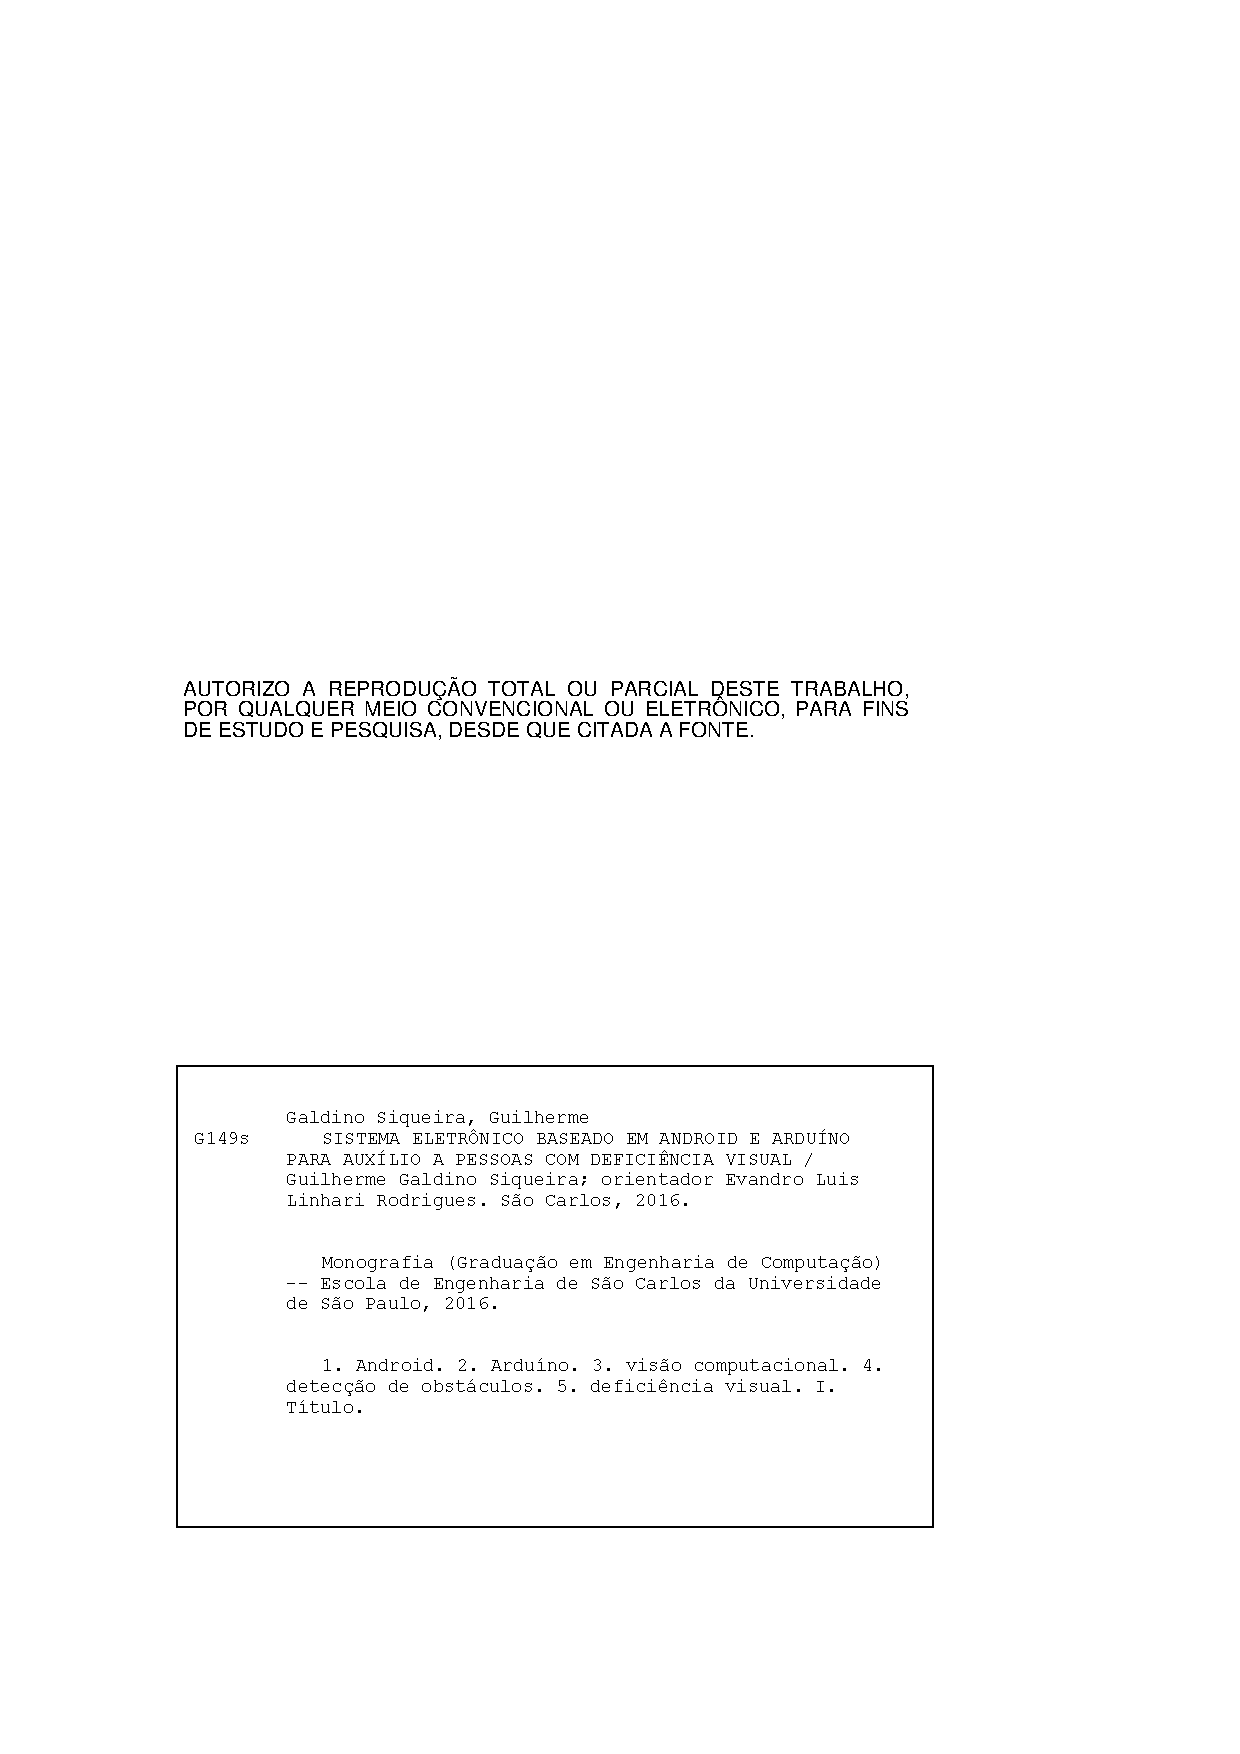
\includepdf{./Resources/ficha.pdf}

% % % % % % % % % % % % % % % % % % % % % % % % Folha de aprova��o % % % % % % % % % % % % % % % % % % %

\newpage


%p�gina com a folha de aprova��o (p�gina �mpar). 
%(normalmente aparece no trabalho final)


\cleardoublepage

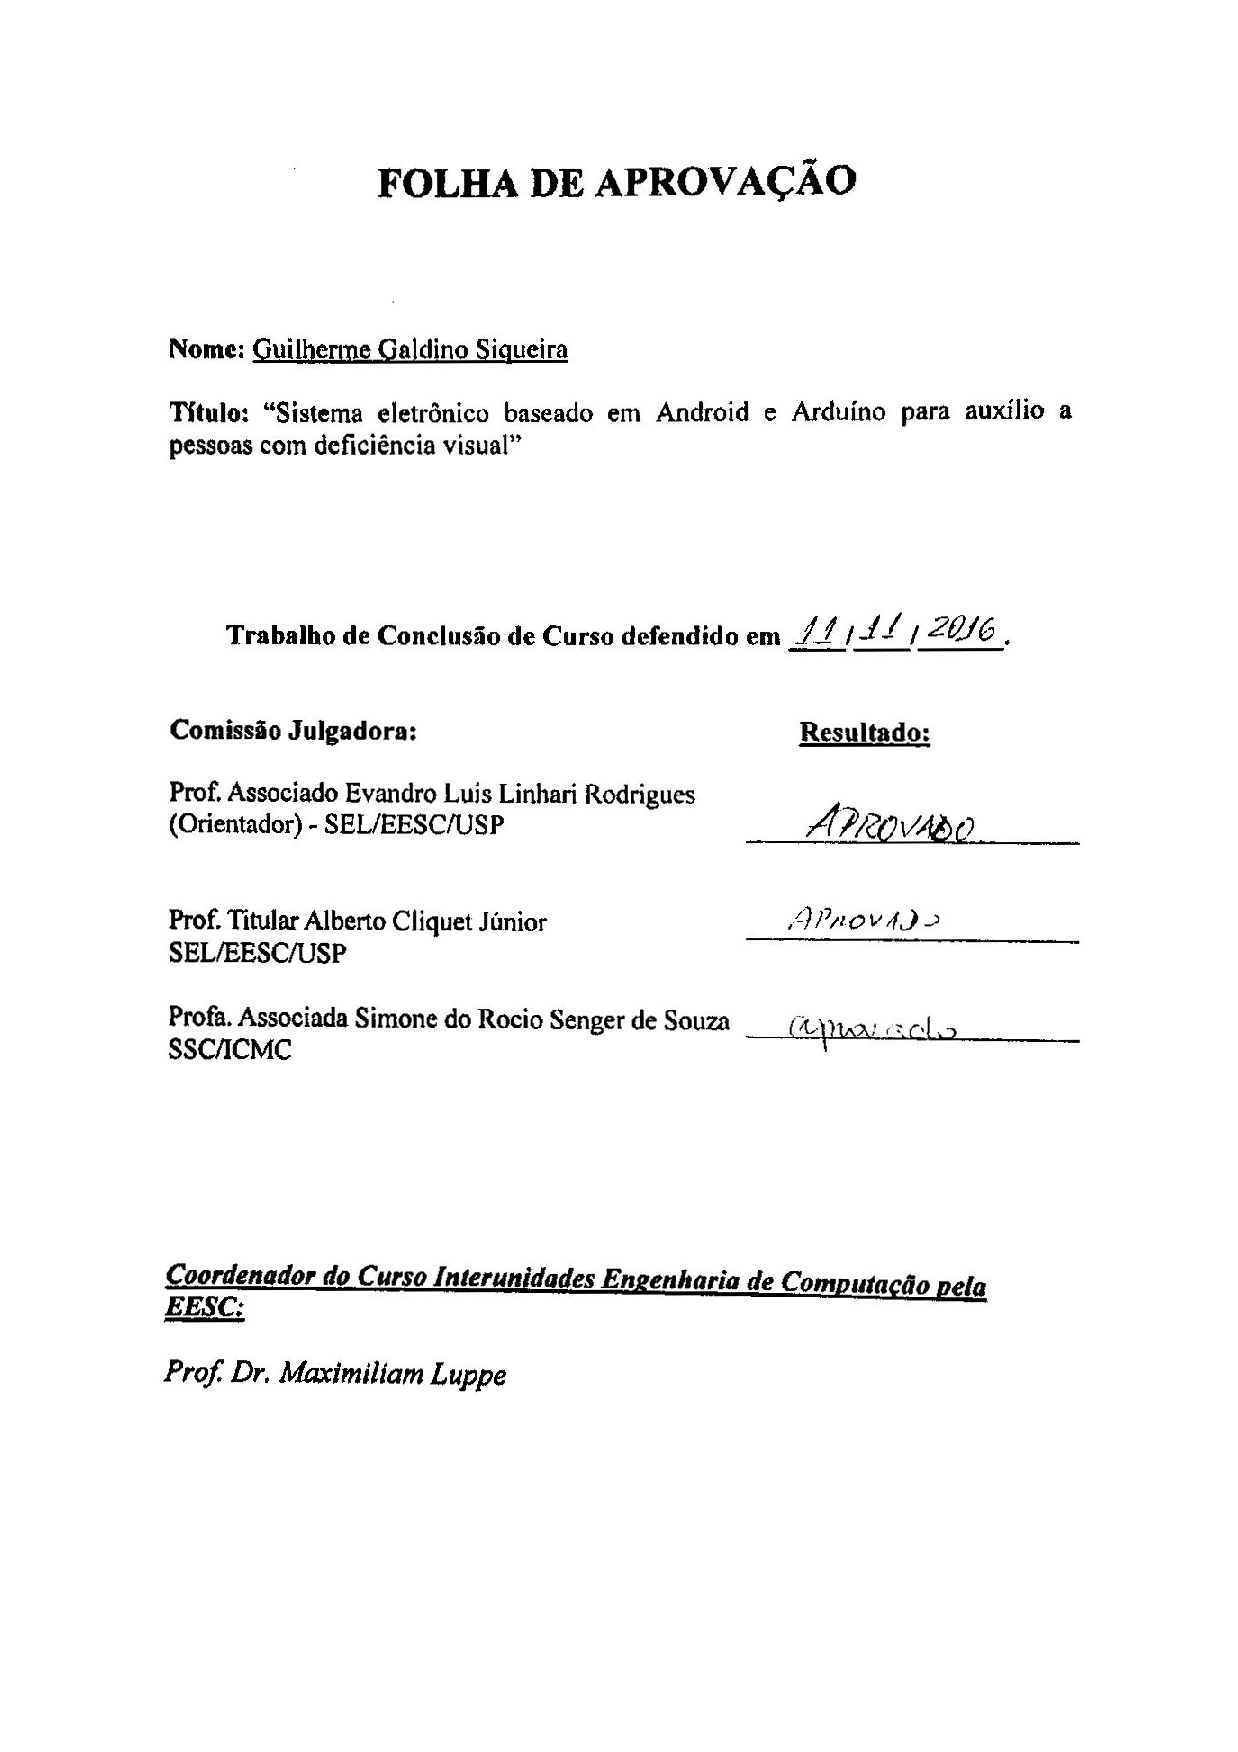
\includepdf{./Resources/aprovacao.pdf}
\cleardoublepage

\begin{comment}
\begin{figure}[H]
	\centering
	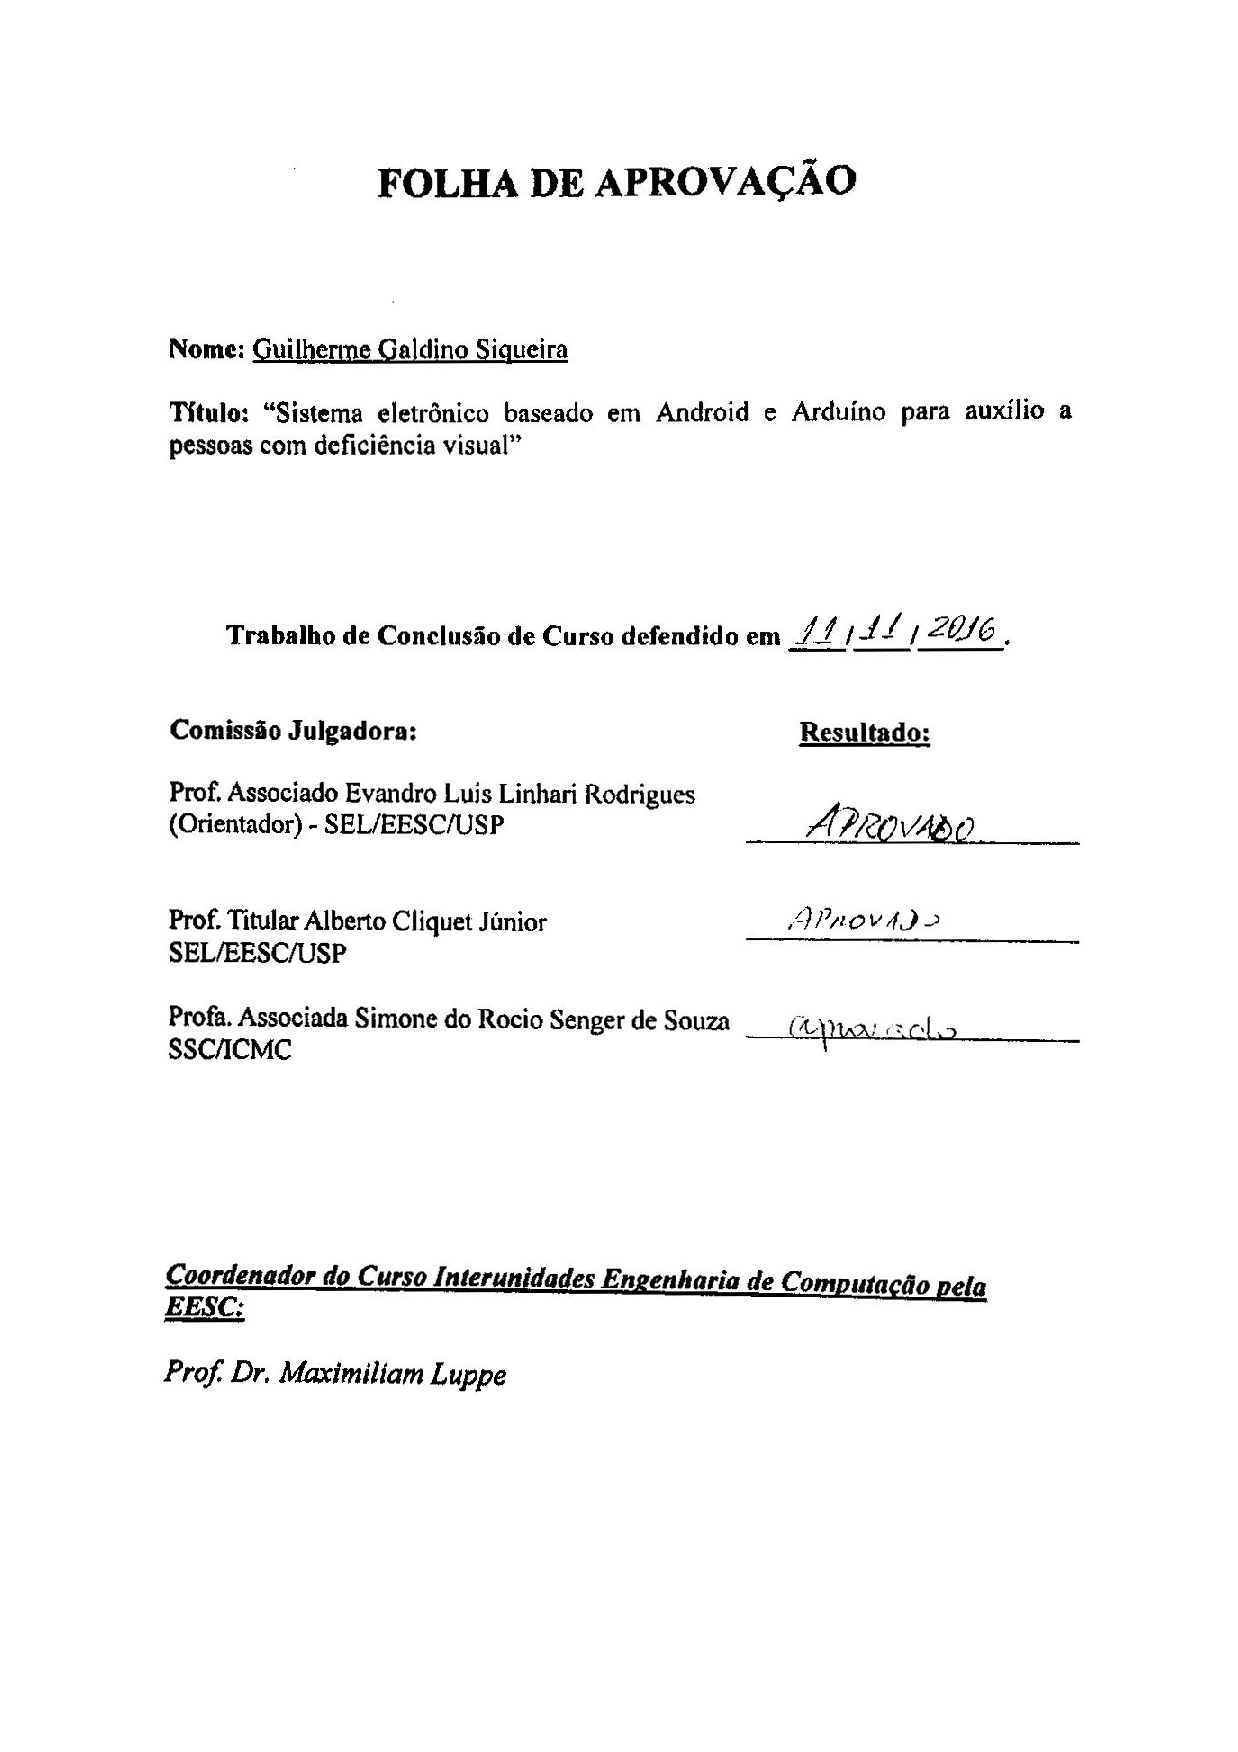
\includegraphics[scale=0.3]{./Resources/aprovacao.jpg}
	\caption{Fluxo de comunica��o entre os principais componentes.}
	\label{Aprovacao}
\end{figure}
\cleardoublepage
\end{comment}



%%%%%%%%%%%%%%%%%%%%%%%%%%%%%%%%%%%%%%%%%%%%%%% DEDICAT?RIA %%%%%%%%%%%%%%%%%%%%%%%%%%%%%%%%%%%%%%%%%%%%%%


\iffalse
\vspace{0.11\textheight} 
\begin{center}
\textbf{\Huge{Dedicat�ria}}
\end{center}
\vspace{0.05\textheight}	
		
A INSERIR
		
\begin{flushright}
Guilherme Galdino Siqueira.
\end{flushright}

%%%%%%%%%%%%%%%%%%%%%%%%%%%%%%%%%%%%%%%%%%%%%%% INSER??O P?GINA EM BRANCO %%%%%%%%%%%%%%%%%%%%%%%%%%%%%%%%%%%%%%%%%%%%%%
\cleardoublepage

\fi
%%%%%%%%%%%%%%%%%%%%%%%%%%%%%%%%%%%%%%%%%%%%%%% AGRADECIMENTOS %%%%%%%%%%%%%%%%%%%%%%%%%%%%%%%%%%%%%%%%%%%%%%
%%\vspace{0.11\textheight} 
\newpage


\begin{center}
\fontsize{16pt}{21pt}\selectfont\bfseries{\textbf{Agradecimentos}}	
\end{center}

						
Agrade�o primeiramente a Deus por todas as vit�rias que obtive antes e durante o per�odo que estive na universidade. Aos meus pais, Marcelo e Ang�lica, e meu irm�o Gabriel por toda paci�ncia e todo apoio que me deram em meio as dificuldades e desafios que enfrentei na gradua��o. � Universidade de S�o Paulo, por abrir diversas portas para minha forma��o, como a oportunidade de estudar no exterior onde come�ou a se formar a ideia desse projeto, e por oferecer a base do meu conhecimento. Agrade�o de modo muito especial meus amigos de turma, com os quais convivi diariamente, e que me deram suporte nos estudos e trabalhos. Ao grupo do Facebook "Cegos e a Tecnologia", pela aten��o dada em alguns momentos de d�vida durante o desenvolvimento do projeto. Agrade�o ao professor Evandro pela confian�a em meu trabalho e por toda orienta��o que me deu no desenvolver desse projeto e, enfim, aos poucos professores que tive que colocaram a preocupa��o com o aprendizado dos alunos acima de tudo em suas avalia��es.


\begin{flushright}
Guilherme Galdino Siqueira
\end{flushright}


%%%%%%%%%%%%%%%%%%%%%%%%%%%%%%%%%%%%%%%%%%%%%%% INSER??O P?GINA EM BRANCO %%%%%%%%%%%%%%%%%%%%%%%%%%%%%%%%%%%%%%%%%%%%%%
\cleardoublepage

%%%%%%%%%%%%%%%%%%%%%%%%%%%%%%%%%%%%%%%%%%%%%%% EP�GRAFE %%%%%%%%%%%%%%%%%%%%%%%%%%%%%%%%%%%%%%%%%%%%%%

%\vspace{0.76\textheight} 

\begin{titlepage}
	
\vspace*{\fill}

\vfill{\begin{flushright}
	
	

		Um homem sozinho n�o desenvolve qualquer poder intelectual. � necess�rio que ele esteja imerso em um ambiente de outros homens, cujas t�cnicas ele absorve durante os primeiros vinte anos de sua vida. Ele pode ent�o talvez realizar alguma pesquisa de sua autoria e fazer pouqu�ssimas descobertas que s�o passadas para outro. Desse ponto de vista, a procura por novas t�cnicas deve ser tratada como realizada pela comunidade humana como um todo, n�o apenas por indiv�duos. 
		
		%%%%%FRASE A INSERIR
		%\textit{"N�s apenas podemos ver a uma curta dist�ncia, mas conseguimos ver o bastante que precisa para ser feito"}
		
		
		Alan Turing

\end{flushright}}

\end{titlepage}


%%%%%%%%%%%%%%%%%%%%%%%%%%%%%%%%%%%%%%%%%%%%%%% INSER??O P?GINA EM BRANCO %%%%%%%%%%%%%%%%%%%%%%%%%%%%%%%%%%%%%%%%%%%%%%

\cleardoublepage

%%%%%%%%%%%%%%%%%%%%%%%%%%%%%%%%%%%%%%%%%%%%%%% RESUMO - PORTUGUES %%%%%%%%%%%%%%%%%%%%%%%%%%%%%%%%%%%%%%%%%%%%%%
%%\
%%\vspace{0.11\textheight} 

\begin{center}
	\fontsize{16pt}{21pt}\selectfont\bfseries{\textbf{Resumo}}	
\end{center}



Este projeto consistiu no desenvolvimento de um sistema composto por um aplicativo para smartphone baseado em Android e uma placa Ardu�no, visando contribuir com a acessibilidade de pessoas sob diferentes n�veis de defici�ncia visual. O sistema oferece ao usu�rio descri��es simples de imagens capturadas pela c�mera do smartphone e oferece suporte de detec��o de obst�culos. O reconhecimento de imagens foi plenamente realizado pela API Google Cloud Vision, que mostrou consider�vel precis�o. A utiliza��o da API permitiu ao projeto seguir a tend�ncia de solicita��o de servi�os em nuvem, por�m tornou o sistema dependente da conex�o com a internet. A detec��o de obst�culos por sua vez exigiu a cria��o de um circuito com a placa Ardu�no conectada a um sensor de obst�culos e um m�dulo Bluetooth. A funcionalidade de detec��o se mostrou eficiente por abranger dist�ncias de at� 4 metros e alertar o usu�rio por sentidos n�o visuais. De modo geral, o sistema mostrou ter boa utilidade e usabilidade.


\vspace{0.05\textheight}
	
Palavras-Chave: Android, Ardu�no, vis�o computacional, detec��o de obst�culos, defici�ncia visual.

%%%%%%%%%%%%%%%%%%%%%%%%%%%%%%%%%%%%%%%%%%%%%%% INSER??O P?GINA EM BRANCO %%%%%%%%%%%%%%%%%%%%%%%%%%%%%%%%%%%%%%%%%%%%%%

\cleardoublepage


%%%%%%%%%%%%%%%%%%%%%%%%%%%%%%%%%%%%%%%%%%%%%%% RESUMO - INGL�S %%%%%%%%%%%%%%%%%%%%%%%%%%%%%%%%%%%%%%%%%%%%%%

\newpage
\begin{center}
	\fontsize{16pt}{21pt}\selectfont\bfseries{\textbf{Abstract}}	
\end{center}	


This project was the development of a system composed of an Android based app and an Arduino board, to contribute to the accessibility of people with different levels of visual impairment. The system provides the user with simple descriptions of images captured by smartphone camera and provides obstacle detection support. The image recognition was totally performed by Google Cloud Vision API, which showed considerable accuracy. The use of the API allowed the project to follow the trend of cloud services request, but made the system dependent on internet connection. The detection of obstacles in turn required the creation of a circuit with the Arduino board connected to an obstacle detection sensor and a Bluetooth module. The detection feature was efficient for covering distances of up to 4 meters and alert the user by nonvisual senses. In general, the system proved to have good utility and usability.

\vspace{0.05\textheight}

Keywords: Android, Arduino, computer vision, obstacles detection, visual impairment.

%%%%%%%%%%%%%%%%%%%%%%%%%%%%%%%%%%%%%%%%%%%%%%% INSER??O P?GINA EM BRANCO %%%%%%%%%%%%%%%%%%%%%%%%%%%%%%%%%%%%%%%%%%%%%%

\cleardoublepage

%\thispagestyle{empty}
%\newpage
%%%%%%%%%%%%%%%%%%%%%%%%%%%%%%%%%%%%%%%%%%%%%%% RESUMO %%%%%%%%%%%%%%%%%%%%%%%%%%%%%%%%%%%%%%%%%%%%%

%%%%%%%%%%%%%%%%%%%%%%%%%%%%%%%%%%%%% CONFIGURA??ES DOS ?NDICES %%%%%%%%%%%%%%%%%%%%%%%%%%%%%%%%%%%%%
%\clearpage
%\thispagestyle{empty}

\listoffigures % ?ndice de Figuras
\listoftables % ?ndice de Tabelas

%%%%%%%%%%%%%%%%%%%%%%%%%%%%%%%%%%%%%%%%%%%%%%% INSER??O P?GINA EM BRANCO %%%%%%%%%%%%%%%%%%%%%%%%%%%%%%%%%%%%%%%%%%%%%%
\cleardoublepage


%%%%%%%%%%%%%%%%%%%%%%%%%%%%%%%%%%%%% LISTA DE ABREVIATURAS %%%%%%%%%%%%%%%%%%%%%%%%%%%%%%%%%%%%%


 

\begin{titlepage}
{
	\vspace{0.11\textheight}
	\raggedleft%
	\textbf{\fontsize{16pt}{5mm}\selectfont\bfseries{Siglas}}
	\vspace{0.05\textheight}
}
{
	\begin{tabbing}
		\hspace*{0.5cm}\=\hspace{2.5cm}\= \kill
		
		% Exemplo de lista de lista de abreviaturas
		\> API \> \textit{Application Programming Interface} - Interface de Programa��o de Aplicativos \\
		\> OCR \> \textit{Optical Character Recognition} - Reconhecimento �tico de Caracter \\
		\> TTS \> \textit{Text-To-Speech} - Texto-Para-Fala \\
		\> IoT \> \textit{Internet of Things} - Internet das Coisas \\
		\> IDE \> \textit{Integrated Development Environment} - Ambiente de Desenvolvimento Integrado \\
		\> ETA \> \textit{Electronic Travel	Aid} - Subs�dio Eletr�nico de Percurso \\
		\> SaaS \> \textit{Software as a Service} - Software como Servi�o \\
		
		
	\end{tabbing}
}
\end{titlepage}


			

\cleardoublepage
%%%%%%%%%%%%%%%%%%%%%%%%%%%%%%%%%%%%% CONFIGURA��ES DOS �NDICES %%%%%%%%%%%%%%%%%%%%%%%%%%%%%%%%%%%%%
%\usepackage{fancyhdr}


\pagestyle{fancy}
\fancyhf{} % clear all header and footer fields
\fancyhead[RO, LE] {\thepage}

\fancypagestyle{plain}{\pagestyle{fancy}}




\setcounter{page}{19}
\tableofcontents % �ndice Geral




%%%%%%%%%%%%%%%%%%%%%%%%%%%%%%%%%%%%%%%% ADI��O DOS CAP�TULOS %%%%%%%%%%%%%%%%%%%%%%%%%%%%%%%%%%%%%%%	
\chapter{Introdu��o}

\label{Introducao}

%\textbf{O CAT, Comit� de Ajudas T�cnicas, institu�do pela PORTARIA N� 142, DE 16 DE NOVEMBRO DE 2006 por meio da Secretaria Especial dos Direitos Humanos, prop�s a seguinte defini��o para o termo Tecnologia Assistiva: "Tecnologia Assistiva � uma �rea do conhecimento, de caracter�stica interdisciplinar, que engloba produtos, recursos, metodologias, estrat�gias, pr�ticas e servi�os que objetivam promover a funcionalidade, relacionada � atividade e participa��o, de pessoas com defici�ncia, incapacidades ou mobilidade reduzida, visando sua autonomia, independ�ncia, qualidade de vida e inclus�o social\cite{LivroTecAss}."}

%\textbf{De forma resumida, a Tecnologia Assistiva consiste em todo o conjunto de ferramentas tecnol�gicas que visam promover a melhoria da qualidade de vida de pessoas com alguma limita��o. Baseado nesse conceito, o projeto procurou seguir a ideia de desenvolver um sistema para atender as necessidades de pessoas com defici�ncia visual.}

Uma pesquisa publicada pelo Banco Mundial em 2016 procurou avaliar simultaneamente os avan�os tecnol�gicos e a exclus�o digital, principalmente com rela��o ao acesso a internet. Seus resultados mostraram que alguns pa�ses est�o muito desvinculados da revolu��o digital, o que reflete na exclus�o socioecon�mica de parcela da popula��o do planeta \cite{WDR}. Esse cap�tulo ter� a intens�o de introduzir o leitor ao cen�rio tecnol�gico atual, a situa��o vivida por pessoas com defici�ncia, apresentar� o estado da arte, por meio de projetos e ir� por fim propor um sistema para aplicar tais tecnologias a esse p�blico alvo.


%Refer�ncia \cite{referencia1}.

%Outra refer�ncia para a bibliografia \cite{referencia2}.

%Segundo \cite{referencia3} h� uma sequ�ncia l�gica para a reda��o da monografia como apresenta em \cite{enzo}.

%ref \cite{referencia5}

%Refer�ncia para a figura \ref{logo}.



% % % % % % % % % % % % % % % % % % % % % % % % % % % % % % % % % % % % % % % % % % % % % % % % % % %
\section{Motiva��o}

No primeiro trimestre de 2016, a aquisi��o mundial de dispositivos m�veis ultrapassou a marca de 7 bilh�es, e esse n�mero permanece em cont�nuo crescimento ano a ano. No mesmo per�odo, foi identificado tamb�m que 80\% de todos os dispositivos m�veis s�o compostos por smartphones e que o n�mero dobrar� at� 2021. A �rea de desenvolvimento de aplica��es m�veis se mostra num momento muito promissor devido n�o s� � quantidade expressiva de dispositivos, que inclusive j� ultrapassa a popula��o de alguns pa�ses, mas tamb�m devido o recente surgimento da Internet das Coisas, IoT \cite{Ericsson}.

Apesar de todo esse progresso, no entanto, muitas pessoas s�o deixadas de lado por n�o terem acesso a esse mundo de possibilidades oferecido pela tecnologia digital. Pessoas com defici�ncia, por exemplo, ainda enfrentam obst�culos para comunica��o, intera��o e acesso a informa��o. A tecnologia atual � capaz de promover diversos meios alternativos de comunica��o desde reconhecimento de voz at� interfaces controladas por gestos. Mas a simples exist�ncia de tecnologia ainda n�o � suficiente para preencher a lacuna de inclus�o socioecon�mica dessas pessoas \cite{WDR}.

A realiza��o desse projeto �, assim, guiada pelo prop�sito de tentar direcionar os benef�cios de uma �rea muito promissora de trabalho, e com in�meras possibilidades de atua��o, a um cen�rio com menor visibilidade, que � o da cria��o de sistemas para o aux�lio a pessoas com defici�ncia, em especial, as visuais.

% % % % % % % % % % % % % % % % % % % % % % % % % % % % % % % % % % % % % % % % % % % % % % % % % % %

\section{Estado da arte}	

Para o desenvolvimento do projeto, diversos projetos bem sucedidos foram utilizados como base. Assim, a proposta procurou seguir a linha de produtos bem sucedidos no mercado na �rea  de aux�lio a pessoas com defici�ncia visual.

 
\subsection{Vis�o computacional}

Na �rea de leitura e extra��o de informa��es de imagens, um exemplo que possui funcionalidades bastantes pr�ximas �s propostas e que serviram de inspira��o � o aplicativo TapTapSee, que fotografa objetos e os identifica em voz alta, al�m de estar vinculado com contas de usu�rio, como Facebook e Twitter para compartilhamento\cite{TapTapSee}.

Existe tamb�m o aplicativo m�vel Be My Eyes, um sistema de aux�lio em rede que conecta usu�rios cegos a volunt�rios por meio de v�deo chamadas e �udio \cite{BeMyEyes}. Mauro Avila et al.\cite{Mauro} faz uma avalia��o do aplicativo que consistiu em uma pesquisa com 15 homens e 15 mulheres atrav�s de m�dias sociais. A maioria dos entrevistados tinha entre 36 e 65 anos de idade. O trabalho concluiu que os usu�rios consideram o aplicativo muito �til para leitura de textos, localiza��o de objetos, assist�ncia a compras, entre outras tarefas do dia a dia.

Outro trabalho bastante interessante � o realizado pela Universidade Hamad Bin Khalifa. H. Kwak e J. An\cite{Kwak} analisaram mais de 2 milh�es de fotos de jornais publicadas em Janeiro de 2016 por meio da API Google Cloud Vision. A pesquisa avaliou a frequ�ncia de exibi��o e express�es faciais em fotos dos ent�o candidatos a presid�ncia dos Estados Unidos, nos principais jornais, e concluiu que a API foi o ponto chave de sucesso do trabalho devido a alta acur�cia e pontua��es de confiabilidade de cada resultado.

\subsection{Ecolocaliza��o}

Na �rea de detec��o de obst�culos, existem diversos projetos ETAs que utilizam sensores ultrass�nicos. Wong et al.\cite{Wong} na intens�o de evitar maus h�bitos de uso da bengala e contornar suas limita��es, prop�s um sistema composto por sensores que continuamente procuram por objetos tamb�m em alturas maiores. O sistema utiliza um microcontrolador para calcular a dist�ncia baseada em sinais ultrass�nicos enviados e recebidos por dois transdutores fixados na bengala, um para detec��o em pequenas alturas, e o outro para grandes. Ent�o depois de emitir os sinais, captura sua reflex�o, calcula a dist�ncia e gera um sinal sonoro de retorno ao usu�rio.

Alternativamente, Ben Leduc-Mills et al\cite{Ben}. apresenta um projeto mais recente envolvendo uma placa IOIO, baseada em PIC, que permite que aplica��es Android interajam com dispositivos eletr�nicos externos. A placa recebe os sinais de sensores ultrass�nicos e os envia ao aplicativo Android via Bluetooth. Ent�o o aplicativo fica respons�vel por tratar o sinal e alertar o usu�rio se h� algum objeto em um limite m�nimo de dist�ncia e a que altura est�. O alerta por fim se d� via audi��o e tato.

% % % % % % % % % % % % % % % % % % % % % % % % % % % % % % % % % % % % % % % % % % % % % % % % % % %

\subsection{Cen�rio no Brasil}

No Brasil tamb�m h� diversos trabalhos nesse sentido.O CPqD Alcance, por exemplo, � um aplicativo que adapta a grande maioria das funcionalidades de um celular em uma interface de maior usabilidade destinado n�o s� para pessoas com defici�ncia visual, mas tamb�m para idosos e pessoas iletradas\cite{CPqD}. 

Na Universidade de S�o Paulo, Murilo A. Gallani\cite{Gallani} apresenta um dispositivo eletr�nico de aprimoramento da orienta��o proporcionada por bengalas � pessoas com defici�ncia visual. O dispositivo, que fica acoplado � ponta de uma bengala, utiliza seu movimento para fazer uma varredura de poss�veis obst�culos, e alerta o usu�rio por meio de sons, cujas intensidades simulam sua emiss�o pelo obst�culo, e auxiliam na localiza��o espacial.

Nessa linha de pesquisa h� tamb�m os projetos Bengala Longa Eletr�nica\cite{UNIVALI} e Bengala Autom�tica para Deficientes Visuais\cite{IFBA}, projetos universit�rios da Universidade do Vale do Itaja� e do Instituto Federal da Bahia, respectivamente, que de maneira similar acoplam a uma bengala sensores que auxiliam na identifica��o de obst�culos.


% % % % % % % % % % % % % % % % % % % % % % % % % % % % % % % % % % % % % % % % % % % % % % % % % % %
\section{Objetivos}


Baseado nos projetos apresentados, esse busca portanto desenvolver mais uma ferramenta alternativa para suprir algumas das necessidades enfrentadas por pessoas com defici�ncia visual, e basicamente prop�e-se a promover ao usu�rio as seguintes habilidades:	

\begin{itemize}  
	\item conhecimento de conte�do visual escrito.
	\item conhecimento de caracter�sticas do ambiente ao redor.	
	\item conhecimento de poss�veis obst�culos pelo caminho.	
	\item maior independ�ncia e autonomia.
\end{itemize}

		






	
	
A Figura \ref{intro} apresenta superficialmente, e de maneira ilustrativa, o que se obteve do sistema proposto quanto a extra��o de informa��es de imagens capturadas. Basicamente, uma aplica��o m�vel ser� capaz, ao capturar uma imagem, de analisar seu conte�do. Textos inseridos em r�tulos de produtos ou bulas de rem�dio, e caracter�sticas faciais ou de paisagens poderiam ser total ou parcialmente compreendidos e com independ�ncia do auxilio de uma pessoa com vis�o normal, por meio da audiodescri��o da informa��o.
	
\begin{figure}[H]
	\centering		
	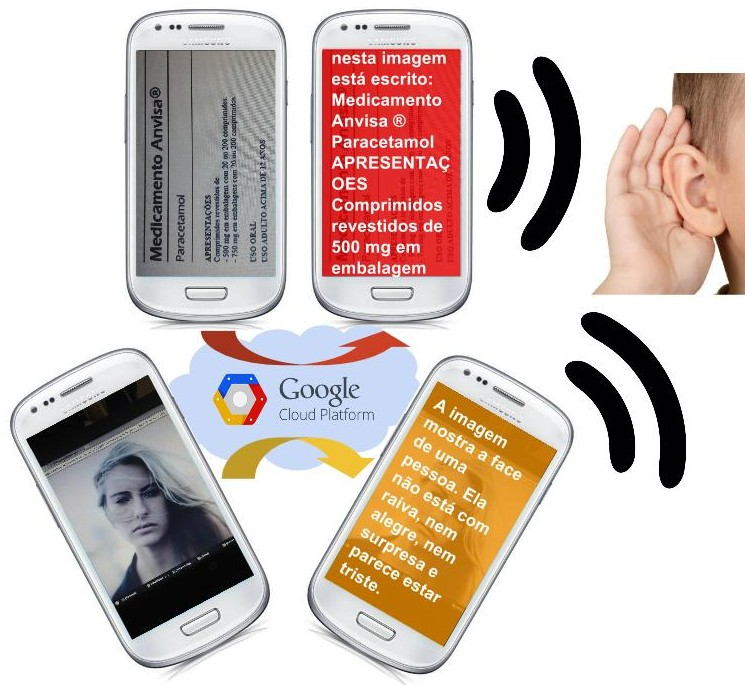
\includegraphics[scale=0.5]{./Resources/intro.jpg}
	\captionof{figure}{Aplicativo - Extra��o de texto e caracter�sticas faciais, respectivos resultados e sa�da sonora para o usu�rio}
	\label{intro}
	
\end{figure} 

J� a Figura \ref{intro2} esquematiza o funcionamento do sistema desenvolvido no cen�rio de uma detec��o de obst�culos durante uma caminhada. Com ele seria poss�vel aumentar a efici�ncia da bengala, ferramenta bastante utilizada por deficientes visuais e que retorna muitas informa��es do ambiente em um percurso. Como obst�culos fora do ch�o nem sempre s�o percebidos pela bengala, o detector de obst�culos poderia servir de aux�lio em situa��es como a ilustrada, em que uma bengala pode at� tocar o suporte do telefone p�blico, mas seria poss�vel que a pessoa chegasse perto demais, e ocorresse uma colis�o entre a cobertura superior e a cabe�a. 

\begin{figure}[H]
	\centering		
	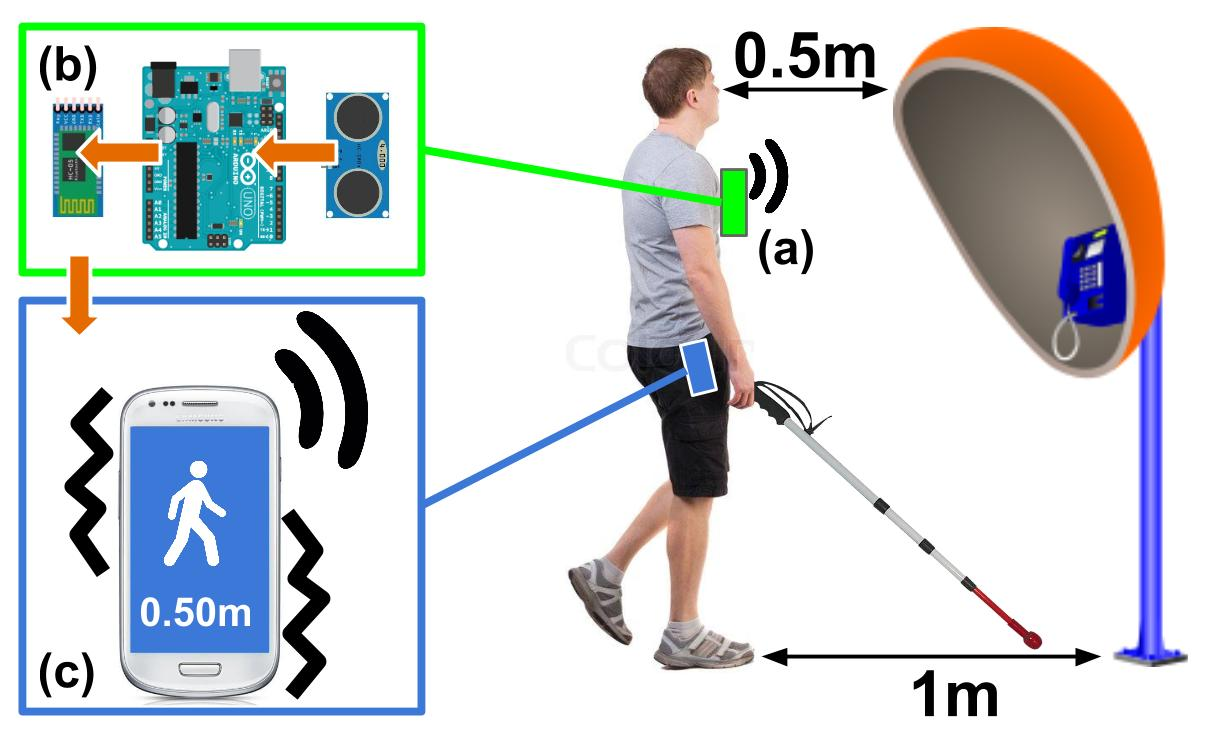
\includegraphics[scale=0.35]{./Resources/intro2.jpg}
	\captionof{figure}{Aplicativo e circuito externo - (a) Gera��o e captura de sinal ultrass�nico, (b) Tratamento do sinal e reenvio para o smartphone, (c) Notifica��o ao usu�rio por vibra��o e som}
	\label{intro2}
	
	\end{figure}	
	
% % % % % % % % % % % % % % % % % % % % % % % % % % % % % % % % % % % % % % % % % % % % % % % % % % %
\section {Justificativas}

Em 2015 o IBGE divulgou dados da Pesquisa Nacional da Sa�de\cite{IBGE} que demostra a propor��o de brasileiros portadores das seguintes defici�ncias: auditiva, visual, f�sica e intelectual. Segundo o levantamento, dentre os tipos de defici�ncia analisados, a visual � a que mais afeta os brasileiros, mais de 3\% da popula��o. A pesquisa tamb�m mostra que 11\% desse grupo � composto por pessoas acima de 60 anos, que quase 7\% utilizam algum recurso de locomo��o, como bengala ou c�o guia, e que o grau intenso de defici�ncia atinge 16\% e resulta na impossibilidade de o indiv�duo realizar tarefas b�sicas, como trabalhar.

Adicionalmente do ponto de vista global, segundo a HDR, Human Development Resources, o Brasil ocupa a posi��o 75 no �ndice de desenvolvimento humano \cite{HDI}. De fato, o pa�s historicamente apresenta algumas dificuldades em promover o bem estar social e a igualdade da popula��o.

Diante desse cen�rio, foi poss�vel perceber que h� uma parcela significativa da popula��o que necessita de aux�lio espec�fico para suprir a falta de vis�o para realizar as mesmas atividades de quem possui vis�o normal. Assim, o desafio desse projeto foi o de desenvolver um sistema que fosse capaz de amenizar as necessidades dessa parcela da popula��o.

Espera-se que com isso seja poss�vel contribuir minimamente com a qualidade de vida a n�vel pessoal de parte da sociedade que possui necessidades especiais e ao mesmo tempo permitir o desempenho da fun��o de engenheiro na sociedade, que � o de colocar o conhecimento cient�fico a servi�o do conforto e desenvolvimento da humanidade.



% % % % % % % % % % % % % % % % % % % % % % % % % % % % % % % % % % % % % % % % % % % % % % % % % % %
\section {Organiza��o do trabalho}

Este trabalho est� distribu�do em 5 cap�tulos, incluindo esta introdu��o, dispostos conforme a descri��o que segue:

\begin{itemize}
	\item Cap�tulo 2: Descreve o embasamento te�rico sobre o qual o projeto foi desenvolvido, definindo conceitos e proporcionando explica��es necess�rias para a compreens�o do desenvolvimento do trabalho.
	\item Cap�tulo 3: Discorre sobre os materiais e m�todos utilizados no andamento do projeto, explicando as caracter�sticas de cada um dos dispositivos eletr�nicos, a raz�o de sua utiliza��o, e o modo como as partes do projeto se conectam entre si. 
	\item Cap�tulo 4: Apresenta os resultados obtidos por meio de teste sobre o sistema, e faz uma an�lise a fim de explic�-los.
	\item Cap�tulo 5: Resume os principais pontos de todo o processo de desenvolvimento at� a finaliza��o do projeto, apresentando a import�ncia da solu��o proposta e os problemas encontrados.
\end{itemize}

 







%\chapter{Especifica��o do Projeto}
\label{Especificacao}

Especifica��o do projeto.


% % % % % % % % % % % % % % % % % % % % % % % % % % % % % % % % % % % % % % % % % % % % % % % % % % %
\section{Se��o 1}

Se��o dentro de um cap�tulo. 



% % % % % % % % % % % % % % % % % % % % % % % % % % % % % % % % % % % % % % % % % % % % % % % % % % %
\section{Se��o 2}

Outra se��o dentro do cap�tulo.


\chapter{Embasamento Te�rico}
\label{EmbasamentoTeorico}

Antes de entender o funcionamento do sistema, � de extrema import�ncia que se explique os principais conceitos que d�o base a cria��o do projeto, a fim de que a leitura n�o se limite apenas a fornecer conhecimento funcional, mas tamb�m propiciar uma completa compreens�o estrutural do sistema. 

\section{Tecnologia assistiva}

O CAT, Comit� de Ajudas T�cnicas, institu�do pela PORTARIA N� 142, DE 16 DE NOVEMBRO DE 2006 por meio da Secretaria Especial dos Direitos Humanos, prop�s a seguinte defini��o para o termo Tecnologia Assistiva: "Tecnologia Assistiva � uma �rea do conhecimento, de caracter�stica interdisciplinar, que engloba produtos, recursos, metodologias, estrat�gias, pr�ticas e servi�os que objetivam promover a funcionalidade, relacionada � atividade e participa��o, de pessoas com defici�ncia, incapacidades ou mobilidade reduzida, visando sua autonomia, independ�ncia, qualidade de vida e inclus�o social\cite{LivroTecAss}."

De forma resumida, a Tecnologia Assistiva consiste em todo o conjunto de ferramentas tecnol�gicas que visam promover a melhoria da qualidade de vida de pessoas com alguma limita��o. Baseado nesse conceito, o projeto procurou seguir a ideia de desenvolver um sistema para atender as necessidades de pessoas com defici�ncia visual.


\section{Design universal e acessibilidade}
Design universal � definido por S. L. Henry et al como o processo de cria��o de produtos que atendam a usabilidade de pessoas com as mais variadas habilidades e nas mais diversas situa��es. Por outro lado, o conceito de acessibilidade � mais limitado, sendo melhor definido como o planejamento voltado especificamente para pessoas com alguma defici�ncia. Apesar disso, todos os estudos focados em acessibilidade terminam por trazer benef�cios para todas as pessoas \cite{Henry}.

Especificamente em rela��o a dispositivos m�veis, ferramentas que permitem a cria��o de sistemas com acessibilidade tem se mostrado em grande ascens�o no ambiente de desenvolvedores de aplicativos. O Android, por exemplo, inclui ferramentas e servi�os de aux�lio a navega��o, como text-to-speech, feedback t�til, navega��o por gestos, entre outros, que buscam incluir usu�rios com limita��es visuais, auditivas, f�sicas ou mesmo relacionadas a idade \cite{Android}.

\subsection{Talkback}

O Talkback � um recurso de acessibilidade fornecido pelo Android cuja fun��o � permitir que deficientes visuais sejam capazes de utilizar um smartphone. Al�m de pronunciar todo tipo de texto presente na tela, ele tamb�m altera a l�gica de toques e permite a descri��o dos componentes presentes no layout.

Quando o Talkback est� ativado, um clique sobre qualquer item da tela funciona como uma solicita��o de descri��o. O dispositivo vibra, o conte�do escrito do item e o texto de acessibilidade, quando h�, s�o pronunciados.



\section{Computa��o em nuvem}
De acordo com a defini��o de Michael Armbrust et al, computa��o em nuvem se refere tanto a aplica��es retornadas como servi�o pela Internet, como ao hardware e software dos sistemas nos data centers que proporcionam os servi�os. Os servi�os s�o oferecidos por software (SaaS), e o conjunto hardware mais software dos data centers d�o origem � nuvem. O servi�o vendido por uma nuvem p�blica � denominado Computa��o Utilit�ria, e sua uni�o com os SaaS �, portanto, o que se conhece como Computa��o em Nuvem \cite{Armbrust}. De maneira simplificada, o funcionamento da computa��o em nuvem pode ser facilmente compreendido pela Figura \ref{Cloud} que, inclusive, permite uma classifica��o do projeto: A Google pode ser vista na base como a provedora de nuvem por oferecer a infraestrutura f�sica necess�ria para o processamento de imagem. No entanto, ela tamb�m pode ser considerada como uma provedora SaaS, por oferecer o Cloud Vision API e diversas outras aplica��es de sua autoria. O aplicativo Android ficaria ent�o exatamente no est�gio intermedi�rio, por oferecer uma aplica��o m�vel como servi�o (SaaS) e ao mesmo tempo por utilizar a nuvem. A pessoa que faz uso desse aplicativo seria, por fim, o usu�rio SaaS.

\begin{figure}[H]
	\centering	
	
	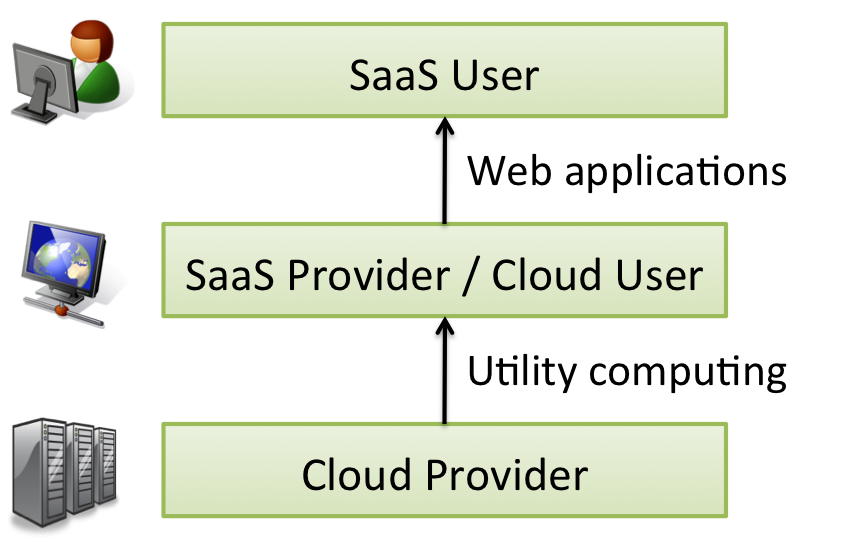
\includegraphics[scale=0.4]{./Resources/cloud.png}
	\captionof{figure}{Diagrama da computa��o em nuvem}
	\caption*{Fonte: Michael Armbrust et al \cite{Armbrust}}	
	\label{Cloud}
	
\end{figure}

\section{Vis�o computacional}
Vis�o computacional � o campo da computa��o respons�vel pela an�lise de imagens digitais com o objetivo da extra��o autom�tica de informa��es. A informa��o pode ser tanto simples, como responder qual a cor da imagem, quanto dizer de quem � a face em uma foto \cite{LivroCV}. No contexto desse projeto, dois pontos importantes devem ser compreendidos: o reconhecimento �ptico de caracteres e a classifica��o de imagens, que s�o apresentados a seguir.


\subsection{Reconhecimento �ptico de caractere}

Reconhecimento �ptico de caractere (OCR) � considerado como o problema de reconhecimento autom�tico de letras, d�gitos, ou algum s�mbolo em imagens. A utilidade dessa abordagem est� no fato de que muita informa��o � armazenada em palavras impressas. Ao aplicar uma p�gina de texto, por exemplo, como entrada para um sistema que possua tal fun��o, ocorre primeiramente uma confirma��o da orienta��o do texto, seguida de uma segmenta��o em preto e branco dos pixels, uma divis�o em linhas de texto, e por �ltimo em s�mbolos individuais. Ao fim desse processo, um algoritmo de reconhecimento � aplicado a cada s�mbolo. Se o sistema tiver sido previamente treinado para reconhecer tal s�mbolo, calcula-se uma probabilidade de sua interpreta��o estar correta, s�o agrupados em palavras e em senten�as e a informa��o completa � retornada em ordem \cite{LivroCV}. Na Figura \ref{OCR}, um simbolo � enviado como entrada do sistema para ser comparado com os s�mbolos da base de dados. Nela, o simbolo apresenta maior similaridade com o s�mbolo '8' (coincid�ncia de 8 pixels), do que com 'A' (coincid�ncia de 20 pixels), e sua classifica��o seria dada de acordo com o s�mbolo com o qual ele tivesse maior valor de semelhan�a, medido pelo n�mero de pixels coincidentes.

\begin{figure}[H]
	\centering	
	
	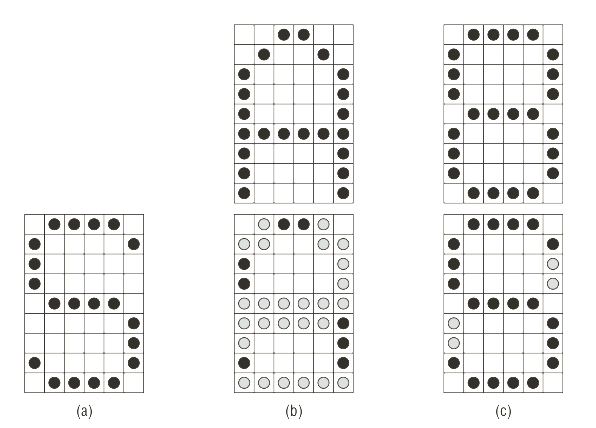
\includegraphics[scale=0.4]{./Resources/ocr.png}
	\captionof{figure}{An�lise de um simbolo sobre a base de dados. (a) Simbolo de entrada. (b) Pixels coincidentes, em preto, entre o simbolo de entrada e o simbolo 'A'. (c) Pixels coincidentes, em preto, entre o simbolo de entrada e o simbolo '8'.}
	\caption*{Fonte: Parker, J. R. \cite{LivroCV}}	
	\label{OCR}
	
\end{figure}

\subsection{Classifica��o de imagens}

Para que um sistema seja capaz de classificar uma imagem, e posteriormente promover uma descri��o, que � o caso desse projeto, � necess�rio que esse sistema esteja previamente treinado com imagens. Um processo como esse, na verdade envolve busca e compara��o de imagens. J. R. Parker sugere em seu livro \cite{LivroCV} um m�todo para se realizar buscas de imagens, inserindo imagens como entrada. 

Primeiramente, assume-se que existe um conjunto de imagens, previamente rotuladas e devidamente classificadas de acordo com seu conte�do. Ent�o, o que ocorre em seguida � uma an�lise computacional da imagem para extra��o de dados. Esses dados s�o comparados com os dados das imagens cujas caracter�sticas j� s�o conhecidas e baseado em sua similaridade, ocorre a classifica��o da imagem, que reflete seu conte�do e que possibilita gerar descri��o. A Figura \ref{imageRecog} ilustra a tentativa de classificar um objeto por meio da medida de semelhan�a contra outras imagens da base de dados. Os mais similares s�o considerados iguais, apesar de o resultado n�o ser exatamente igual.

\begin{figure}[H]
	\centering	
	
	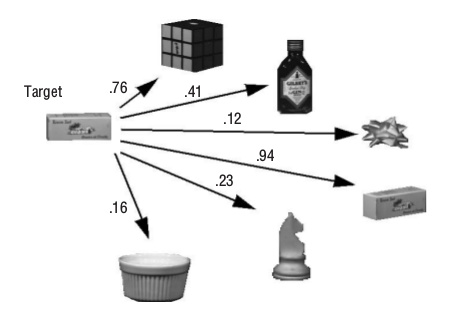
\includegraphics[scale=0.5]{./Resources/imageRecog.png}
	\captionof{figure}{Classifica��o de imagem de acordo com sua similaridade em rela��o ao conjunto de imagens da base de dados.}
	\caption*{Fonte: Parker, J. R. \cite{LivroCV}}	
	\label{imageRecog}
	
\end{figure} 

Uma pergunta que poderia surgir �: Que informa��o poderia ser extra�da de uma imagem para servir de crit�rio de compara��o? A cor � uma possibilidade. Atrav�s da contagem de pixels com cada cor presente na imagem � poss�vel criar um histograma da distribui��o dessas cores. E assim, a compara��o poderia ser realizada sobre a similaridade entre histogramas.



\section{Ecolocaliza��o e localiza��o sonora}

A habilidade de se locomover independentemente pelo espa�o, localizar lugares ocultos e planejar trajet�rias � de extrema import�ncia para se realizar as tarefas do cotidiano. N�o � dif�cil encontrar raz�es para afirmar que essa capacidade, em pessoas, resulta em grande depend�ncia do sentido visual, j� que a quantidade de informa��es que podem ser captadas visualmente � consideravelmente maior que a dos outros sentidos. Os objetos com os quais se interage no dia-a-dia possuem partes vis�veis, por�m n�o necessariamente emitem outros sinais que possam permitir sua percep��o n�o visual. Apesar de ser considerada uma medida muito mais imprecisa, sinais sonoros permitem uma aproxima��o do c�lculo de distancia. O som varia sua intensidade ao se propagar de acordo com o inverso da dist�ncia at� seu emissor, assim, sua intensidade se perde mais rapidamente, o que a torna um m�todo limitado \cite{blind}.

A localiza��o sonora se baseia nesse efeito, ao permitir que um indiv�duo estime a sua dist�ncia at� o objeto emissor de som, e � uma t�cnica utilizada e bastante desenvolvida por pessoas com defici�ncia visual para mapear a sua posi��o e a dos elementos no ambiente ao redor. Entretanto, existe tamb�m uma t�cnica capaz de complementar a efici�ncia da localiza��o conhecida como ecolocaliza��o. � sabido que os humanos, e especificamente pessoas cegas, s�o capazes de utilizar o eco de sons intencionalmente emitidos para detectar objetos e conseguir andar. Esse fen�meno que tamb�m � encontrado em outras esp�cies de animais, como golfinho e morcego, por exemplo, podem ser gerados n�o s� biologicamente pela voz, mas tamb�m por toques com sapatos ou bengalas \cite{echo}.







%{Existem diversos projetos ETAs que utilizam sensores ultrass�nicos. Wong et Al. na intens�o de evitar maus h�bitos de uso da bengala e contornar suas limita��es, prop�s um sistema composto por sensores que continuamente procuram por objetos tamb�m em alturas maiores. O sistema utiliza um microcontrolador para calcular a dist�ncia baseada em sinais ultrass�nicos enviados e recebidos por dois transdutores fixados na bengala, um para detec��o em pequenas alturas, e o outro para grandes \cite{Wong}. Ent�o depois de emitir os sinais, captura sua reflex�o, calcula a dist�ncia e gera um sinal sonoro de retorno ao usu�rio.

%Alternativamente, Ben Leduc-Mills et Al. apresenta um projeto mais recente envolvendo uma placa IOIO, baseada em PIC, que permite que aplica��es Android interajam com dispositivos eletr�nicos externos \cite{Ben}. A placa recebe os sinais de sensores ultrass�nicos e os envia ao aplicativo Android via Bluetooth. Ent�o o aplicativo fica respons�vel por tratar o sinal e alertar o usu�rio se h� algum objeto em um limite m�nimo de dist�ncia e a que altura est�. O alerta por fim se d� via audi��o e tato.


%H� tamb�m diversos projetos com foco na transcri��o de informa��es de imagens. Mauro Avila et al faz uma avalia��o do aplicativo m�vel Be My Eyes \cite{BeMyEyes}, um sistema em rede que conecta usu�rios cegos a volunt�rios por meio de v�deo chamadas e �udio. O trabalho realizou uma pesquisa com 15 homens e 15 mulheres atrav�s de m�dias sociais. A maioria dos entrevistados tinha entre 36 e 65 anos de idade. O trabalho concluiu que os usu�rios consideram o aplicativo muito �til para leitura de textos, localiza��o de objetos, assist�ncia a compras, entre outros \cite{Mauro}.

%Outro trabalho bastante interessante � o realizado pela Universidade Hamad Bin Khalifa. H. Kwak e J. An analisaram mais de 2 milh�es de fotos de jornais publicadas em Janeiro de 2016 por meio da API Google Cloud Vision. A pesquisa avaliou a frequ�ncia de exibi��o e express�es faciais em fotos dos ent�o candidatos a presid�ncia dos Estados Unidos, nos principais jornais, e concluiu que a API foi o ponto chave de sucesso do trabalho devido a alta acur�cia e pontua��es de confiabilidade de cada resultado \cite{Kwak}.


%Baseado nos trabalhos apresentados, nota-se que para a transcri��o de informa��es de imagens, o Google Cloud API � uma boa alternativa. Quanto a funcionalidade de detec��o de obst�culos, a utiliza��o de sensor ultrass�nico mostra-se como a solu��o mais adequada ao problema.}

\chapter{Material e M�todos}
\label{Materiais}

Mais do que uma simples aplica��o Android, o projeto englobou o sensoreamento de sinais ultrass�nicos, comunica��o sem fio e um circuito gerenciado por um Ardu�no. Por essa raz�o, diversos componentes eletr�nicos e m�todos de comunica��o foram utilizados.	

Basicamente, o usu�rio do smartphone, por meio do aplicativo Android captura uma imagem daquilo que deseja obter informa��es. A imagem � enviada aos servidores em nuvem da Google, onde � processada e tem suas informa��es traduzidas lexicograficamente. O resultado � ent�o transferido de volta para o smartphone e apresentado em forma textual apropriada sob a qual pode se obter uma audiodescri��o. 

Por outro lado, um sensor conectado a um Ardu�no emite ondas ultrass�nicas periodicamente e retorna a dist�ncia estimada ao obst�culo. O resultado � ent�o transferido ao smartphone, por meio de um m�dulo BlueTooth tamb�m conectado ao Ardu�no, e a aplica��o por fim alerta o usu�rio. A figura \ref{esquematico} apresenta um esquem�tico que exemplifica o funcionamento do sistema.

 \begin{figure}[H]
 	\centering
 	
 	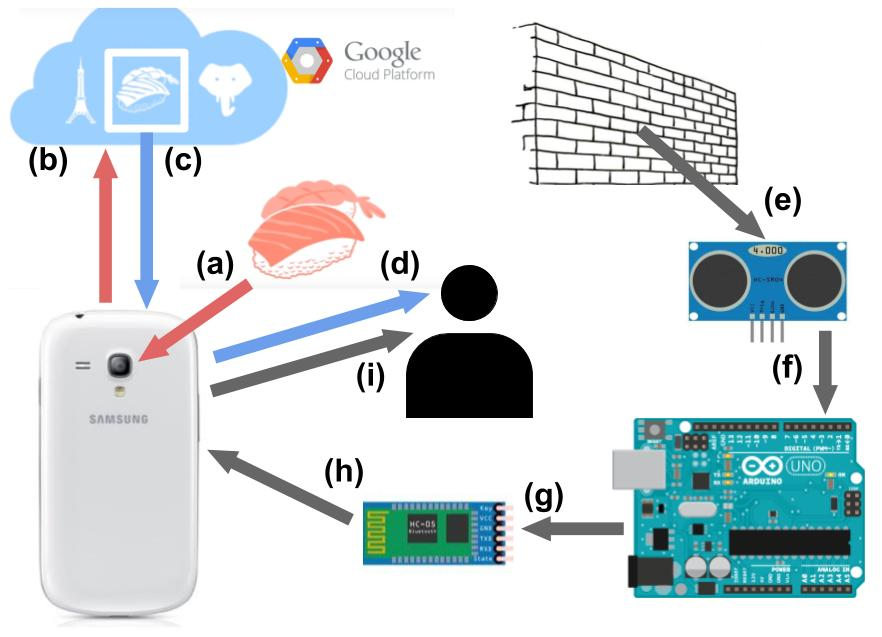
\includegraphics[scale=0.35]{./Resources/esquematico1.jpg}
 	%\caption*{Fonte: Autor}
 	\captionof{figure}{Esquem�tico de comunica��o entre os m�dulos eletr�nicos do projeto}
 	\label{esquematico}
 \end{figure}


% % % % % % % % % % % % % % % % % % % % % % % % % % % % % % % % % % % % % % % % % % % % % % % % % % %
\section{Materiais}

Os materiais utilizados, bem como a descri��o detalhada de suas propriedades e sua fun��o no projeto est�o listados a seguir.

\subsection{Smartphone}
 \begin{figure}[H]
 	\centering
 	
 	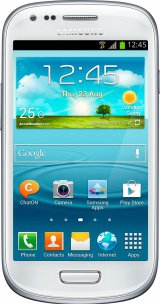
\includegraphics[scale=0.35]{./Resources/smartphone.jpg}
 	\captionof{figure}{Smartphone Galaxy S3 mini}
 	\caption*{Fonte: www.tudocelular.com}
 	
 	\label{PhotoSmartphone}
 \end{figure}
O n� principal do sistema pode ser considerado o smartphone. Por ser um dispositivo multifuncional com c�mera, sa�da de �udio, vibra��o e permitir a execu��o de aplicativos, al�m de possuir tamanho mais reduzido se comparado ao tablet, por exemplo, mostrou-se ideal para o prop�sito do projeto. Com a c�mera foi poss�vel a captura das imagens posteriormente tratadas para extra��o de informa��o. A sa�da de �udio em paralelo com a vibra��o foram essenciais para uma interface �til voltada para usu�rios com defici�ncia visual. O tamanho reduzido tamb�m foi importante para que o dispositivo pudesse manuseado e guardado facilmente no corpo. Bastou ent�o o desenvolvimento de um aplicativo que gerenciasse todos os recursos de hardware necess�rios. O smartphone utilizado majoritariamente durante o desenvolvimento do projeto foi o Samsumg Galaxy S3 mini \ref{PhotoSmartphone}, cuja especifica��o t�cnica est� descrita na tabela \ref{dataSmartphone}.

\begin{table}[]
	\centering
	\caption{Especifica��o t�cnica do smartphone utilizado no projeto}
	\label{dataSmartphone}
	\begin{tabular}{ll}
		   
		Sistema Operacional  & Android 4.1 Jelly Bean   \\
		Dimens�es            & 121.55 x 63 x 9.85 mm    \\  
		Peso                 & 111.5 g 					\\   
		RAM                  & 1 GB   					\\    
		Mem�ria              & 16 GB 					\\   
		Resolu��o - C�mera   & 2592 x 1944 pixel   		\\ 
     
	\end{tabular}
\end{table}

\subsection{Android Studio}
Uma vez que o smartphone escolhido para o projeto foi o Galaxy S3 mini, cujo sistema operacional � o Android, para a programa��o do aplicativo foi necess�ria a utiliza��o da IDE Android Studio 1.4.

\subsection{Ardu�no}

\begin{figure}[H]
	\centering
	
	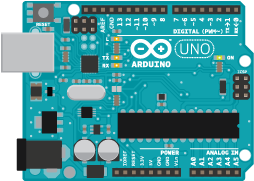
\includegraphics[scale=0.35]{./Resources/arduino.jpg}
	\captionof{figure}{Ardu�no UNO}
	\caption*{Fonte: www.arduino.cc}
	\label{PhotoArduino}
\end{figure}

Para a funcionalidade de detec��o de obst�culos, que n�o poderia ser feita pelo smartphone, foi necess�ria a utiliza��o de outro dispositivo. Para tanto, foi definido que essa funcionalidade poderia ser facilmente realizada pela placa de programa��o Ardu�no UNO, figura \ref{PhotoArduino}. As especifica��es da placa est�o na tabela \ref{dataArduino}.

\begin{table}[]
	\centering
	\caption{Especifica��o t�cnica Ardu�no}
	\label{dataArduino}
	\begin{tabular}{ll}
		
		Microcontrolador     & ATmega328P   	\\
		Pinos de E/S         & 14           	\\  
		Dimens�es			 & 68.6 x 53.4 mm	\\
		Peso                 & 25 g 			\\
		Flash Memory		 & 32 KB			\\
		SRAM				 & 2 KB				\\
		EEPROM				 & 1 KB 			\\  		
		
	\end{tabular}
\end{table}

\subsection{Sensor}

\begin{figure}[H]
	\centering
	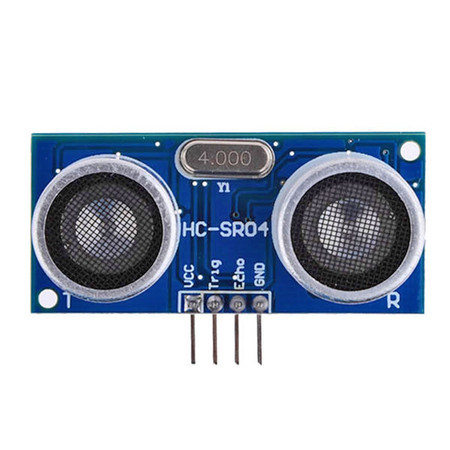
\includegraphics[scale=0.2]{./Resources/sensor.jpg}
	\captionof{figure}{Sensor HC-SR04.}
	\caption*{Fonte: www.filipeflop.com}
	
	\label{PhotoSensor}
\end{figure}

O Ardu�no como uma placa program�vel, possibilita um infinidade de aplica��es. Entretanto ele n�o possui sensores acoplados, apenas entradas e sa�das gen�ricas. Para a detec��o de obst�culos foi necess�ria a inser��o de um sensor. O HC-SR04, figura \ref{PhotoBlueTooth}, sensor ultrass�nico que se mostrou eficiente para a tarefa desejada. Emitindo ondas de frequ�ncia ultrass�nica, o sensor capta o sinal refletido e baseado na intensidade permite o c�lculo da dist�ncia.

\subsection{BlueTooth}

\begin{figure}[H]
	\centering
	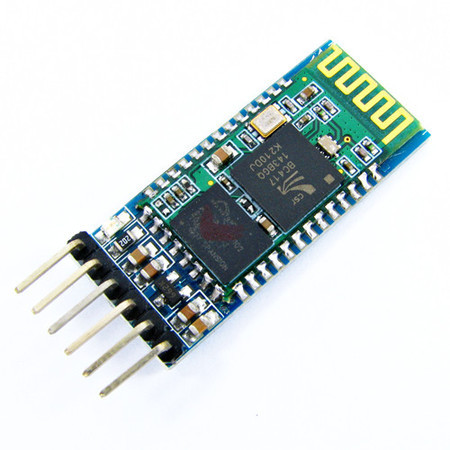
\includegraphics[scale=0.2]{./Resources/bluetooth.jpg}
	\captionof{figure}{M�dulo BlueTooth HC-05.}
	\caption*{Fonte: www.filipeflop.com}
	\label{PhotoBlueTooth}
\end{figure}

Para a comunica��o entre o Ardu�no e o smartphone haviam diversas possibilidades de implementa��o. A troca de dados pela internet j� seria utilizada pela aplica��o Android para o reconhecimento de imagens, que ser� apresentado com mais detalhes na se��o M�todos. No entanto, havia solu��es mais simples, como por exemplo, a comunica��o via BlueTooth, adota pelo projeto. Assim como o sensor, foi inserido ao circuito controlado pelo Ardu�no o m�dulo BlueTooth HC-05, apresentado pela figura \ref{PhotoBlueTooth}.

\subsection{Componentes eletr�nicos em geral}

Para a conex�o dos componentes do circuito foram necess�rios uma variedade de fios. No total foram utilizados por volta de 10 unidades para conectar VCC, GND, emendas e conex�es de entrada e sa�da de sinais. Foram necess�rios tamb�m resistores para cria��o de um divisor de tens�o. Para tanto foram utilizados tr�s resistores de 220$\Omega$ para transformar 5V em 3V. Al�m disso, para fixar os componentes e montar o circuito, foram utilizados fita isolante e um suporte de pl�stico. Para a programa��o do circuito utilizou-se um cabo USB. Os componentes citados s�o mostrados na Figura \ref{componentes}.



% % % % % % % % % % % % % % % % % % % % % % % % % % % % % % % % % % % % % % % % % % % % % % % % % % %
\section{M�todos}

Os m�todos utilizados para a se atingir o objetivo do projeto s�o extremamente importantes n�o s� para a compreens�o de como as partes se comunicam, mas tamb�m para se expor detalhes da implementa��o que s�o essenciais para garantir ampla usabilidade e acessibilidade do usu�rio.

\subsection{Configura��es iniciais de programa��o}

Antes de tudo, para o in�cio da programa��o do aplicativo foi necess�ria a instala��o do Android Studio e para a programa��o da placa Ardu�no, da IDE de mesmo nome. 

\subsection{Constru��o de interface acess�vel}

O objetivo do projeto era permitir que pessoas com limita��es visuais pudessem exercer algumas fun��es exclusivas de pessoas que podem ver. Por essa raz�o, o ponto mais importante, e primeiro a ser planejado foi a interface. Ent�o, a primeira coisa a ser feita era definir se o Android 4.1 permitiria a usabilidade por pessoas a qual o projeto se destina.

\begin{figure}[H]
	\centering
	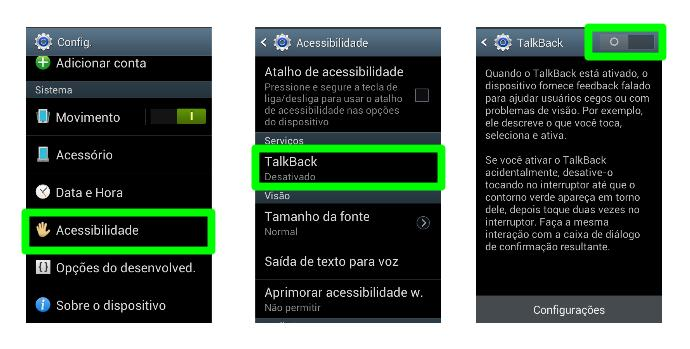
\includegraphics[scale=0.5]{./Resources/talkback.jpg}
	\caption{Talkback}
	\label{PhotoTalkback}
\end{figure}

A princ�pio, foi considerada a possibilidade de implementar tradu��o de texto em �udio pela aplica��o. Dessa forma, qualquer informa��o na tela do aplicativo poderia ser descrita ao usu�rio pelo som. No entanto isso foi desnecess�rio quando entrou em cena o Talkback, figura \ref{PhotoTalkback}, servi�o nativo do Android que adapta a l�gica de intera��o para pessoas com dificuldades de vis�o. Al�m de fazer automaticamente a tradu��o texto-�udio de qualquer informa��o presente na tela, o Talkback muda a l�gica de cliques e insere sons e vibra��es de resposta a qualquer a��o realizada, desde toques em bot�es at� deslizamento em listas. Com isso, o projeto pode avan�ar para outro ponto importante da interface: o tamanho dos elementos.

\begin{figure}[H]
	\centering
	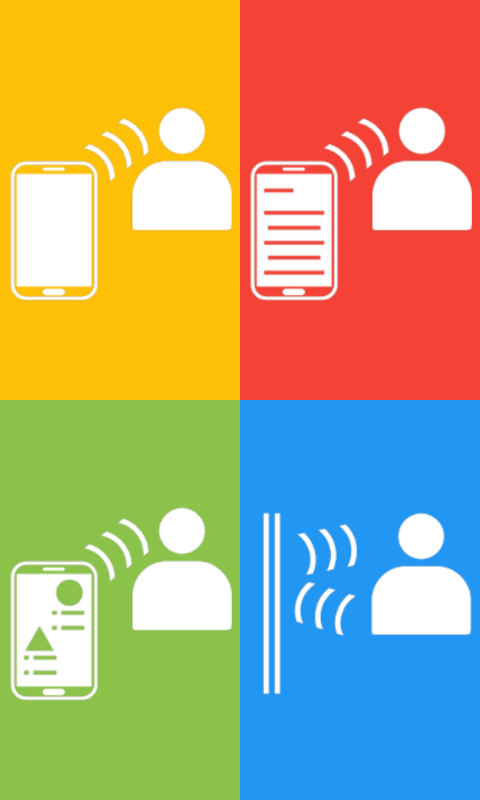
\includegraphics[scale=0.3]{./Resources/menu.png}
	\caption{Tela inicial do aplicativo}
	\label{menu}
\end{figure} 

Uma das dificuldades enfrentadas por essas pessoas ao utilizar aplicativos � selecionar o elemento correto na tela devido o tamanho reduzido em rela��o aos dedos. Por essa raz�o, o menu principal, Figura \ref{menu}, divide a tela toda em quatro grandes �reas que servem para posicionamento dos bot�es. Al�m disso, a barra de status do Android e de t�tulo do aplicativo foram ocultadas, para garantir o melhor aproveitamento de espa�o da tela. 

Outro problema a ser considerado foi a navegabilidade. Um dos requisitos para que uma pessoa sem vis�o pudesse utilizar um aplicativo � saber onde est�, ou seja, impedir que o usu�rio n�o se perdesse na sequ�ncia de menus. Por isso, al�m de n�o haver submenus na interface, o padr�o de desenvolvimento de aplica��es Android foi respeitado, com a inser��o de descri��o de conte�do a todos os elementos da interface, como mostra a Figura \ref{nav}. Essas descri��es ficam visualmente ocultas, mas s�o lidas apenas pelo Talkback, que transforma a informa��o em �udio.

\begin{figure}[H]
	\centering
	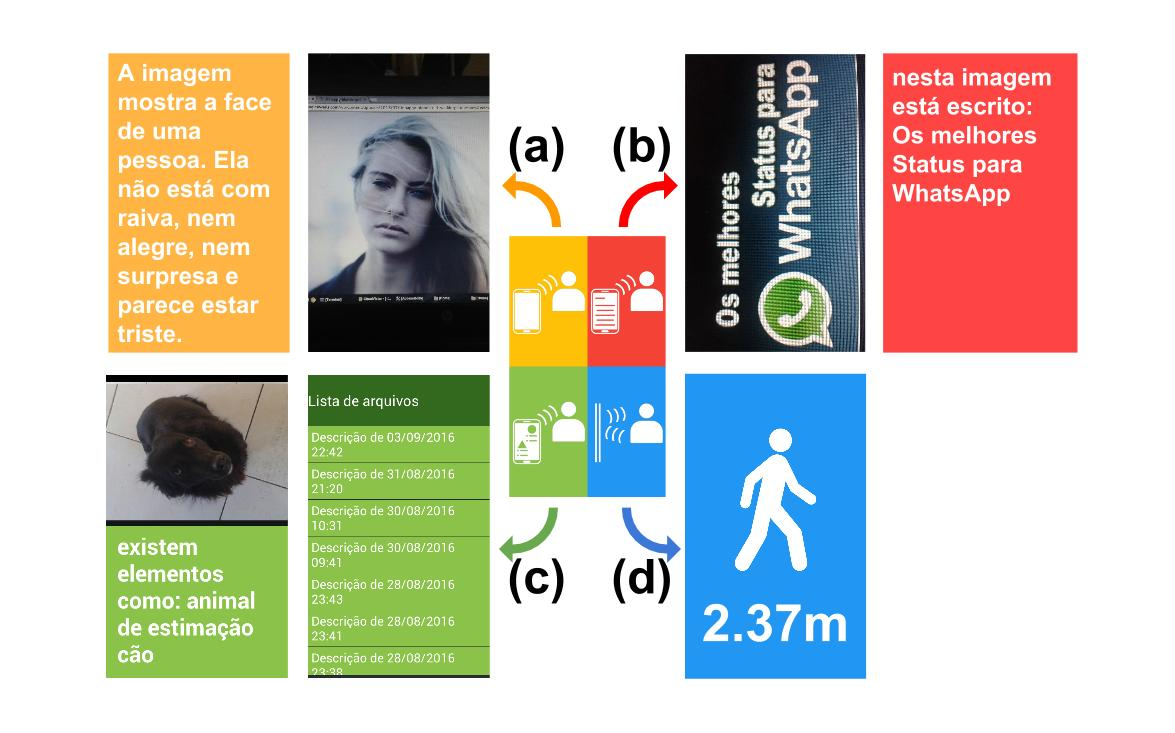
\includegraphics[scale=0.35]{./Resources/navegabilidade.jpg}
	\caption{Tela principal e respectivas funcionalidades. (a) Descri��o facial. (b) Extra��o de texto (c) Sele��o de registros (d) Detec��o de obst�culos}
	\label{nav}
\end{figure} 

Uma vez que o aplicativo n�o se limita a atender apenas pessoas com aus�ncia total de vis�o, outro cen�rio considerado foi a utiliza��o do aplicativo por pessoas com graus mais menos intensos de defici�ncia visual. Baseado na pesquisa de acessibilidade realizada por Shaun K. Kane et al com pessoas de diferentes graus de falta de vis�o, fontes de tamanho grande e o contraste de cores s�o considerados caracter�sticas importantes \cite{Kane}. Assim, um esquema de cores bastante fortes e contrastantes foram utilizadas. E cada cor utilizada nos bot�es do menu principal foi tamb�m utilizada como cor de fundo da interface correspondente � op��o selecionada. Al�m disso, o tamanho das letras dos textos de resultado foi aumentado significativamente e formatado em negrito para facilitar uma poss�vel leitura.

Implementadas todas as caracter�sticas de acessibilidade no aplicado, o resultado foi:


\begin{itemize}
	\item Interface que permite �udio descri��o;
	\item Menu principal, com apenas quatro bot�es e cores contrastantes;
	\item Bot�o que acessa a c�mera e exibe a descri��o com o m�ximo de informa��es da imagem capturada;
	\item Bot�o que acessa a c�mera e exibe apenas textos da imagem capturada;
	\item Bot�o que leva a uma lista de descri��es salvas e permite acess�-las;
	\item Bot�o que inicia conex�o com o Ardu�no;
	\item Menu de op��es que permite inserir ou remover alguns sons/anima��es de resposta;
\end{itemize}

\subsection{Extra��o de dados em imagem}

A solu��o adotada para o reconhecimento de dados em imagem foi o Cloud Vision, uma API em nuvem da Google de reconhecimento de imagens, e com gratuidade limitada ao n�mero de requisi��es mensais, cujos valores podem ser encontrados na Tabela \ref{Price}. Como o projeto a princ�pio n�o � um produto e n�o � de grande porte, n�o exigiria muitas requisi��es e se mostrou uma solu��o muito adequada. 

\begin{figure}[H]
	\centering
	
	\captionof{table}{Pre�os da API Google Cloud Vision por quantidade e tipo de solicita��o}
	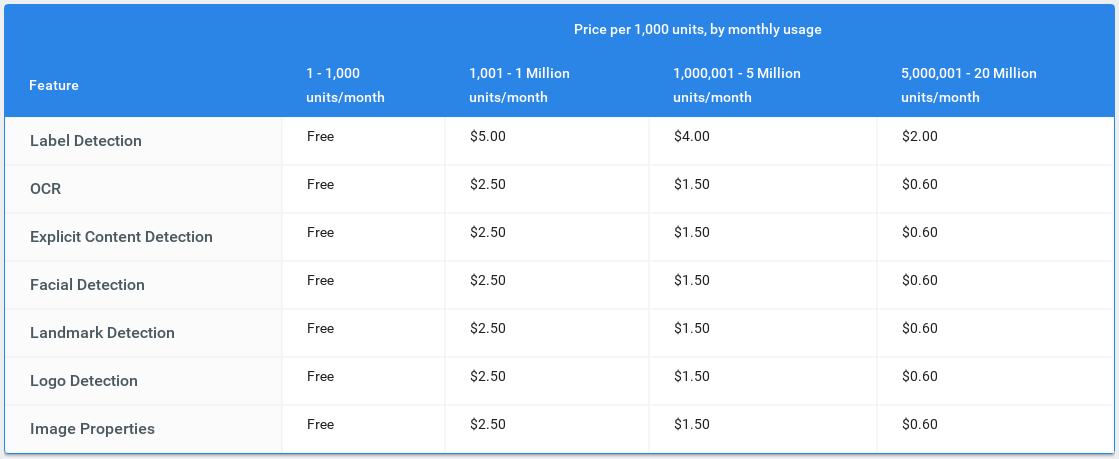
\includegraphics[scale=0.4]{./Resources/price.png}
	\caption*{Fonte: Google Cloud Platform\cite{bestPracticesGoogle}}
	
	\label{Price}
	
\end{figure}

A API criada em 2015 apesar de muito potente e ter atra�do muitos usu�rios interessados em automatizar a classifica��o de imagens, ainda n�o tem aparecido com muita frequ�ncia em trabalhos cient�ficos. Entretanto, para demonstrar as capacidades da API, a Google apresentou na GCP NEXT 2016 o projeto Cloud Vision Explorer, um ambiente web gal�ctico contendo milhares de imagens separadas por categorias, que utiliza o Cloud Vision que � modelado pelo TensorFlow, uma biblioteca de software livre para intelig�ncia de m�quina tamb�m pertencente a Google \cite{Galaxy}.

Para se ter acesso aos servi�os da Google Cloud, � necess�rio se cadastrar no sistema. Uma vez dentro do sistema, foi criado um projeto sobre o Vision API. Em seguida, para permitir a utiliza��o desse projeto pela aplica��o Android, foi necess�rio gerar uma chave de identifica��o de API. Por meio da importa��o dos pacotes em linguagem Java e dessa chave, bastou a constru��o de objeto de chamada de servi�o no aplicativo. Logo depois, associou-se ao objeto a imagem fonte, o modo de compress�o e de codifica��o da imagem a ser enviada, o portugu�s como idioma de identifica��o de textos e por fim as categorias que se poderia buscar na imagem, entre elas, texto, r�tulo e express�es faciais. Com o objeto configurado, bastou enviar a requisi��o ao servidor da Google e aguardar o resultado. Ao final do processo, o retorno da requisi��o veio em um objeto contendo as informa��es pedidas separadas por categorias e suas respectivas pontua��es de confian�a. 

\subsection{Adapta��o textual do dado retornado}

Ap�s utilizar os servi�os do Cloud Vision para a extra��o de informa��es da imagem, o passo seguinte foi adaptar as informa��es escritas para um conte�do textual de f�cil compreens�o. O motivo � que as informa��es extra�das vinham em partes, separadas por categorias, nem sempre vinham preenchidas com informa��o, ou mesmo possu�am probabilidade baixa de estarem corretas podendo ser descartadas. Assim, foi necess�rio filtrar esses dados, adicionando um limite de 80\% de confiabilidade. Tamb�m, para garantir uma boa flu�ncia no texto resultante, as informa��es foram filtradas por categoria e dependendo da qual pertencessem, produziriam uma sa�da textual espec�fica.

\subsection{Tradu��o de r�tulos}
Outra adapta��o necess�ria foi em rela��o ao idioma. Apesar de a ferramenta ser capaz de identificar um infinidade deles, os resultados retornados de r�tulos relacionadas a imagem estavam sempre em ingl�s. A solu��o encontrada foi traduzir esses r�tulos antes de compor a sa�da textual final. No entanto, n�o h� suporte diretamente do Android para essa funcionalidade, e seguindo o exemplo da solicita��o de servi�os online, a solu��o encontrada foi utilizar novamente alguma API de tradu��o. Como a API de tradu��o da Google n�o oferece faixa de solicita��es gratuitas, o que � extremamente importante, utilizou-se em vez disso a API de tradu��o Yandex, figura \ref{Yandex}, que assim como a Cloud Vision oferecia um limite de gratuidade.

\begin{figure}[H]
	\centering
	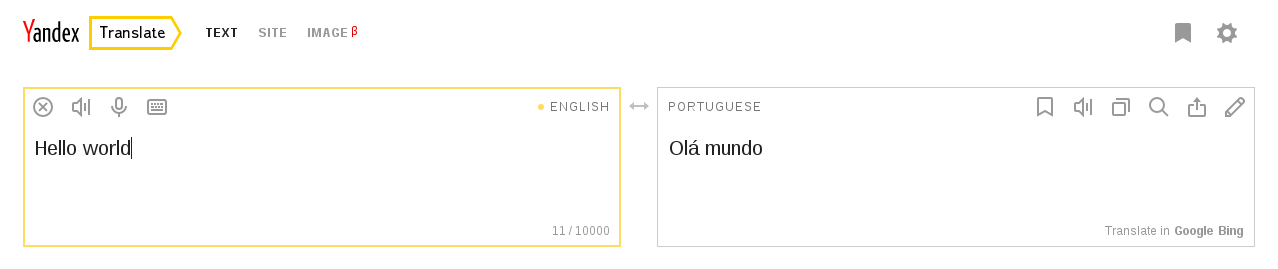
\includegraphics[scale=0.35]{./Resources/yandex.png}
	\caption{Interface gr�fica do Tradutor Yandex acessado pelo navegador}
	\label{Yandex}
\end{figure}

\subsection{Captura e exibi��o de resultado}
O processo de descri��o de imagem inicia-se em uma tela que exibe as imagens vindas da c�mera traseira do smartphone. O aplicativo, por�m, n�o requisita em momento algum acesso a c�mera frontal. Com um toque, ou dois quando o Talkback est� ativado, o aplicativo captura a imagem, a salva no dispositivo no formato JPG, em uma nova pasta dentro do diret�rio do aplicativo e a envia para a nuvem. Enquanto o aplicativo aguarda o retorno do servi�o solicitado, uma imagem de rel�gio pisca suave e lentamente na tela, enquanto um som de tic-tac � tocado como forma de informar o usu�rio que ele deve aguardar o processo. Tamb�m, a imagem capturada mant�m-se como plano de fundo durante todo o processo de espera.

\begin{figure}[H]
	\centering
	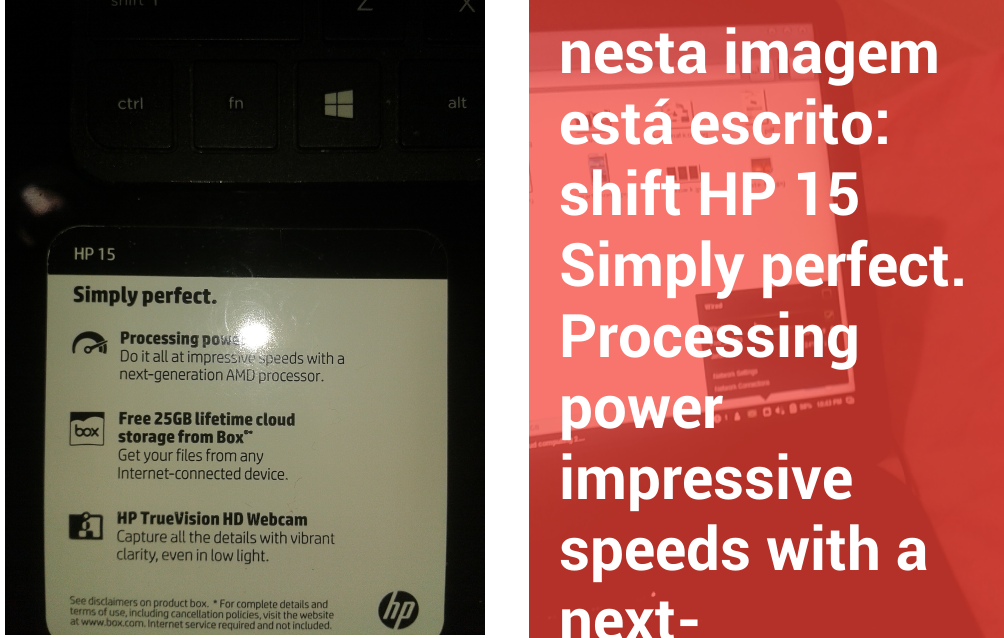
\includegraphics[scale=0.4]{./Resources/capRes.png}
	\caption{Imagem capturada e seu respectivo resultado}
	\label{CapRes}
\end{figure} 

Quando o resultado enfim chega ao aplicativo, a anima��o e o som de processamento s�o interrompidos, o plano de fundo volta a mostrar as imagens da c�mera, e sobre ela, abre-se uma caixa de texto transl�cida e desliz�vel, conforme mostra a Figura \ref{CapRes}, contendo o texto descritivo em negrito e em fonte grande. Com um longo clique, ou no caso do Talkback estar ativado, um curto clique seguido de um longo sobre a tela, o texto � copiado para a �rea de transfer�ncia. O bot�o de retorno permite ao usu�rio voltar a c�mera, e o bot�o de menu, o permite ativar ou desativar os efeitos visual e sonoro realizados durante a espera do processamento. Ao final, a descri��o � salva na mesma pasta da imagem capturada.

\subsection{Implementa��o de op��es de reconhecimento}
Com todo o tratamento dado ao conte�do transcrito das imagens, para essa funcionalidade, foram criadas duas op��es ligeiramente distintas para o aplicativo, como ilustra a Figura \ref{funcoes}. A primeira requisitaria apenas detec��o de caracteres da imagem capturada com o intuito de reduzir o n�mero de requisi��es, e possivelmente reduzir o tempo de resposta. Essa funcionalidade seria aplic�vel no caso espec�fico de o usu�rio ter o conhecimento pr�vio de que a imagem poderia estar preenchidas por algum texto, e que essa informa��o sozinha pudesse ser relevante e suficiente.
A segunda funcionalidade solicitaria todas as informa��es poss�veis ao Cloud Vision, que s�o: Textos, R�tulos, Logotipos, e Pontos tur�sticos. Por fim, ambas alternativas de extra��o de informa��o da imagens foram inseridas em dois dos quatro bot�es do menu principal.

\begin{figure}[H]
	\centering
	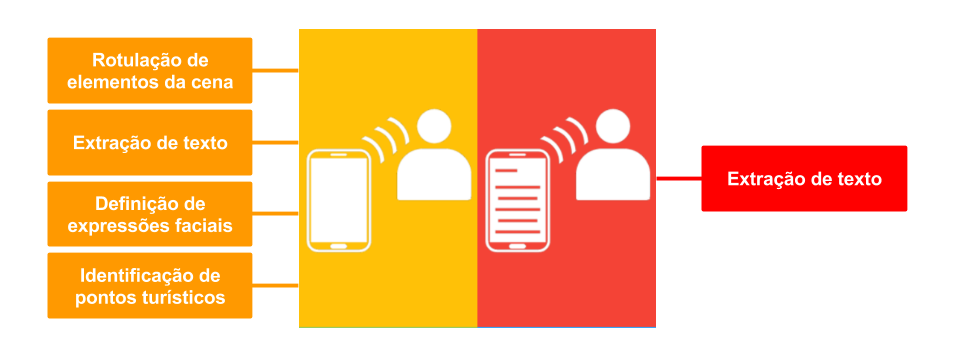
\includegraphics[scale=0.45]{./Resources/funcoes.png}
	\caption{Compara��o entre bot�es de solicita��o de extra��o de informa��o de imagem}
	\label{funcoes}
\end{figure} 




\subsection{Registro de descri��es}

A funcionalidade de transcri��o de imagem em texto foi perfeitamente realizada. Mas para prover ao usu�rio a possibilidade de resgatar resultados anteriores, foi importante permitir que o aplicativo oferecesse a op��o de salvar. Nesse ponto surgiu uma quest�o: Qual seria melhor forma de usu�rio acessar esse registro? 

Nomear os registros com parte da descri��o poderia causar ambiguidade de nomes e poderia dificultar encontr�-los caso houvesse muitos. Assim, foi decidido que os registros seriam nomeados com a data e hora de cria��o. Al�m disso, seriam sempre ordenados temporalmente ao serem carregados na lista pelo aplicativo. Isso facilitou muito o acesso, pois os mais recentes apareciam no topo, e data/hor�rio s�o identificadores �nicos e permitem f�cil localiza��o na procura por um registro. A Figura \ref{select} apresenta uma lista de registros que foi gerada pela utiliza��o do aplicativo.

Com isso decidido, foi necess�rio planejar a estrutura desse registro. A princ�pio considerou-se que o �udio referente � transcri��o deveria ser salvo. No entanto, o prop�sito principal do aplicativo era apenas extrair informa��es de imagens e encontrar uma forma de fazer com que o usu�rio com defici�ncia visual pudesse acess�-la. Salvar o �udio deixou de ser necess�rio quando se percebeu que a fun��o de �udio descri��o � parte exclusiva da interface de acessibilidade do aplicativo, e n�o � obrigat�ria para todos os usu�rios. A inten��o de salvar os dados n�o � pela voz da �udio descri��o, mas exclusivamente por seu conte�do.

Assim, cada registro correspondia a um diret�rio contendo apenas a foto no formato JPG, para refer�ncia de quem pode ver, e um arquivo no formato TXT contendo a descri��o. A �udio descri��o ficou sob responsabilidade da interface, ap�s o carregamento do registro. Por fim, essa funcionalidade foi atribu�da a um dos quatro bot�es do menu principal. 

\begin{figure}[H]
	\centering
	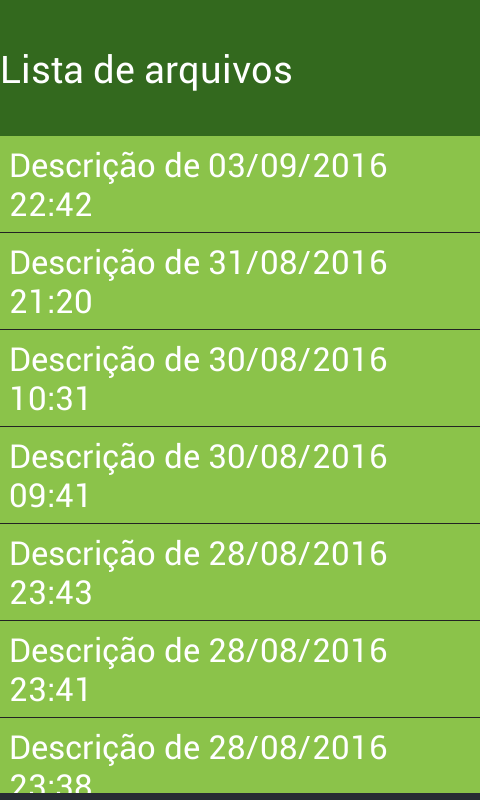
\includegraphics[scale=0.4]{./Resources/select.png}
	\caption{Lista de registros de descri��o}
	\label{select}
\end{figure} 


\subsection{Tratamento de sinais ultrass�nicos}
O tratamento de sinais vindos do sensor HC-SR04 � parte essencial do projeto, por�m a mais simples de ser feita. Do ponto de vista de hardware, o sensor possui quatro pinos de conex�o: VDD, GND, Trigger e Echo. O VDD foi conectado a alimenta��o de 5V do Ardu�no, assim como o GND conectado ao terra. O Trigger e o Echo s�o respectivamente entrada e sa�da do sensor para que o sensor receba comando para emiss�o de ondas de 40 kHz de frequ�ncia e ent�o retorne em sua sa�da o valor medido da reflex�o da onda. Esses dois pinos foram conectados respectivamente nos Pinos 4 e 5 do Ardu�no.

Do ponto de vista l�gico, o programa que roda no Ardu�no basicamente controla a emiss�o e recep��o de sinais do sensor, e em seguida repassa para o m�dulo Bluetooth. O sensor aguarda a onda refletida, e baseado no tempo entre emiss�o e recep��o, � poss�vel calcular a dist�ncia percorrida at� o obst�culo. O sensor tem capacidade de identificar obst�culos at� 4 metros. Quando ocorre algum erro de medida, e a dist�ncia calculada � maior que esse limite, o valor � ignorado e n�o � reenviado ao Bluetooth.

\subsection{Comunica��o Arduino-BlueTooth}

Para transmitir sinais do Ardu�no para o smartphone via m�dulo BlueTooth, bastou inserir a informa��o na porta Serial. O mais importante foi, na verdade, decidir que informa��o deveria ser transmitida. Para garantir a modularidade do sistema, o Ardu�no ficou encarregado apenas de enviar ininterruptamente os sinais lidos pelo sensor ao smartphone, sem realizar qualquer verifica��o de proximidade de obst�culos, fun��o que o aplicativo Android ficou encarregado de fazer.

Do ponto de vista de circuitos, apenas quatro dos seis pinos do m�dulos foram utilizados. A raz�o foi que o HC-05 pode ser programado para ser mestre ou escravo. No modo escravo, os pinos KEY e STATE podem ser ignorados, e como n�o havia necessidade de o Ardu�no se conectar a nenhum outro dispositivo, nem mesmo de requisitar conex�es, esse foi o modo adotado para o BlueTooth no sistema. Foram ent�o conectados VCC e GND aos respectivos pinos do Ardu�no, para alimentar o m�dulo. O pino TXD de transmiss�o do m�dulo foi conectado ao pino RX do Ardu�no, para recep��o de sinais de comunica��o vindos do smartphone. Por fim, o pino TX do Ardu�no foi conectado ao RXD do m�dulo. Para adaptar a tens�o de sa�da do Ardu�no � tens�o adequada do m�dulo, foi necess�rio implementar um circuito divisor de tens�o, pois o sinal proveniente do Ardu�no � de 5V por�m a tens�o recomendada do m�dulo � da ordem de 3V.

\subsection{Comunica��o Smartphone-BlueTooth}

Do lado oposto da comunica��o, no aplicativo Android foi necess�rio receber os dados do Ardu�no. Para tanto, um ciclo de comandos foi executado em plano de fundo. Primeiramente, o BlueTooth era ligado e fazia-se uma varredura repetitiva de dispositivos ao redor. Caso encontrasse um com o nome HC-05, a varredura era interrompida e tentava-se iniciar um conex�o. Ao ser iniciada, o aplicativo iniciava uma leitura contante do buffer de entrada e o dado, dist�ncia at� um poss�vel obst�culo, era tratado e gerava-se duas poss�veis classifica��es: Surgimento de obst�culos no caminho ou Desaparecimento de obst�culos no caminho, ambos baseados em um limite m�nimo definido de 1m. Quando um dos dois casos ocorresse, um alerta seria emitido, o qual seria lido pelo Talkback para informar o usu�rio. Essa funcionalidade por fim foi colocada com a��o do �ltimo dos quatro bot�es do menu principal.

O circuito completo, contendo o sensor de obst�culos, o m�dulo bluetooth e o Ardu�no, pode ser visualizado na figura \ref{circuit}.


\begin{figure}[H]
	\centering
	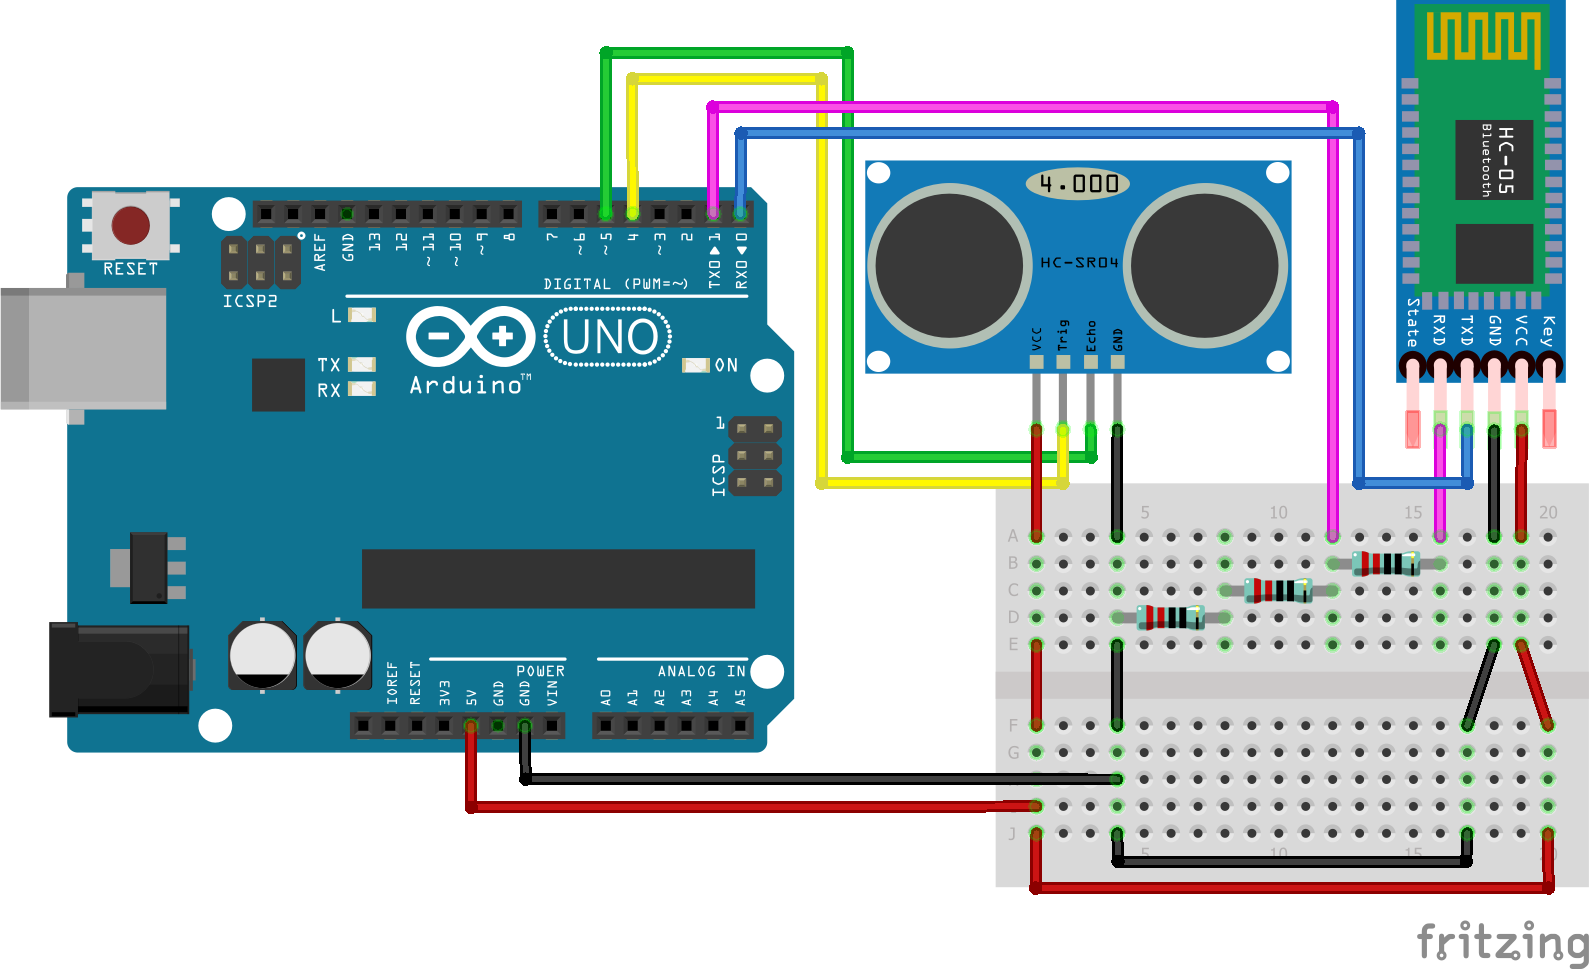
\includegraphics[scale=0.7]{./Resources/circuit.png}
	\caption{Circuito Ardu�no com m�dulo BlueTooth e sensor de obst�culos}
	\label{circuit}
\end{figure}





\chapter{Resultados e Discuss�es}
\label{Resultados}

Com as funcionalidades planejadas para o projeto conclu�das, o passo seguinte foi a realiza��o de testes. Esse cap�tulo ser� dividido em duas se��es tal que na primeira ser�o tratados dos resultados da extra��o de informa��o de imagens, e a segunda, tratar� da performance do detector de obst�culos.

\section{Descri��o de Imagens}

Na descri��o de imagens duas considera��es foram necess�rias para garantir o correto desempenho do sistema: o tempo de resposta, pois n�o � conveniente deixar o usu�rio esperando por muito tempo pela informa��o requisitada, e a qualidade dos resultados obtidos, para que o usu�rio receba aquilo que � esperado do sistema. Como a Google Cloud API � uma ferramenta online, a primeira dificuldade encontrada para efici�ncia de processamento foi o transporte de dados para o servidor da Google. Quanto mais dados s�o transmitidos pela rede e processados pela rotina no servidor, maior o tempo de lat�ncia para a resposta. Isso significa que a velocidade da Internet do usu�rio ser� sempre um limitador. 


\subsection{Teste para diferentes dimens�es de imagens}

Apesar de a velocidade da internet ser um fator limitante, a quantidade de dados transmitida, em alguns casos, pode ser flexibilizada uma vez que a imagem pode ter sua resolu��o reduzida e exibir um n�mero menor de bytes para ser representada. Entretanto, essa redu��o resulta em um detalhamento menor da imagem, o que pode dificultar seu processamento, causar erros de interpreta��o de seu conte�do e por fim n�o retornar resultados satisfat�rios. A fim de confrontar resolu��o de imagem, tempo de processamento e qualidade dos resultados, para cada solicita��o de extra��o de informa��o das imagens, a mesma imagem foi enviada com diversas resolu��es, e os tempos das fases do processo foram medidos. A Figura \ref{Teste-HP} cont�m a imagem capturada para esse fim. Como � poss�vel observar a partir da Tabela \ref{Estat-HP} juntamente com o resultado exibido pela Figura \ref{Resultado-HP}, a resolu��o da imagem � proporcional ao tempo total de processamento da informa��o requisitada e inversamente proporcional a quantidade de erros do resultado. 

\begin{figure}[H]
	\centering
	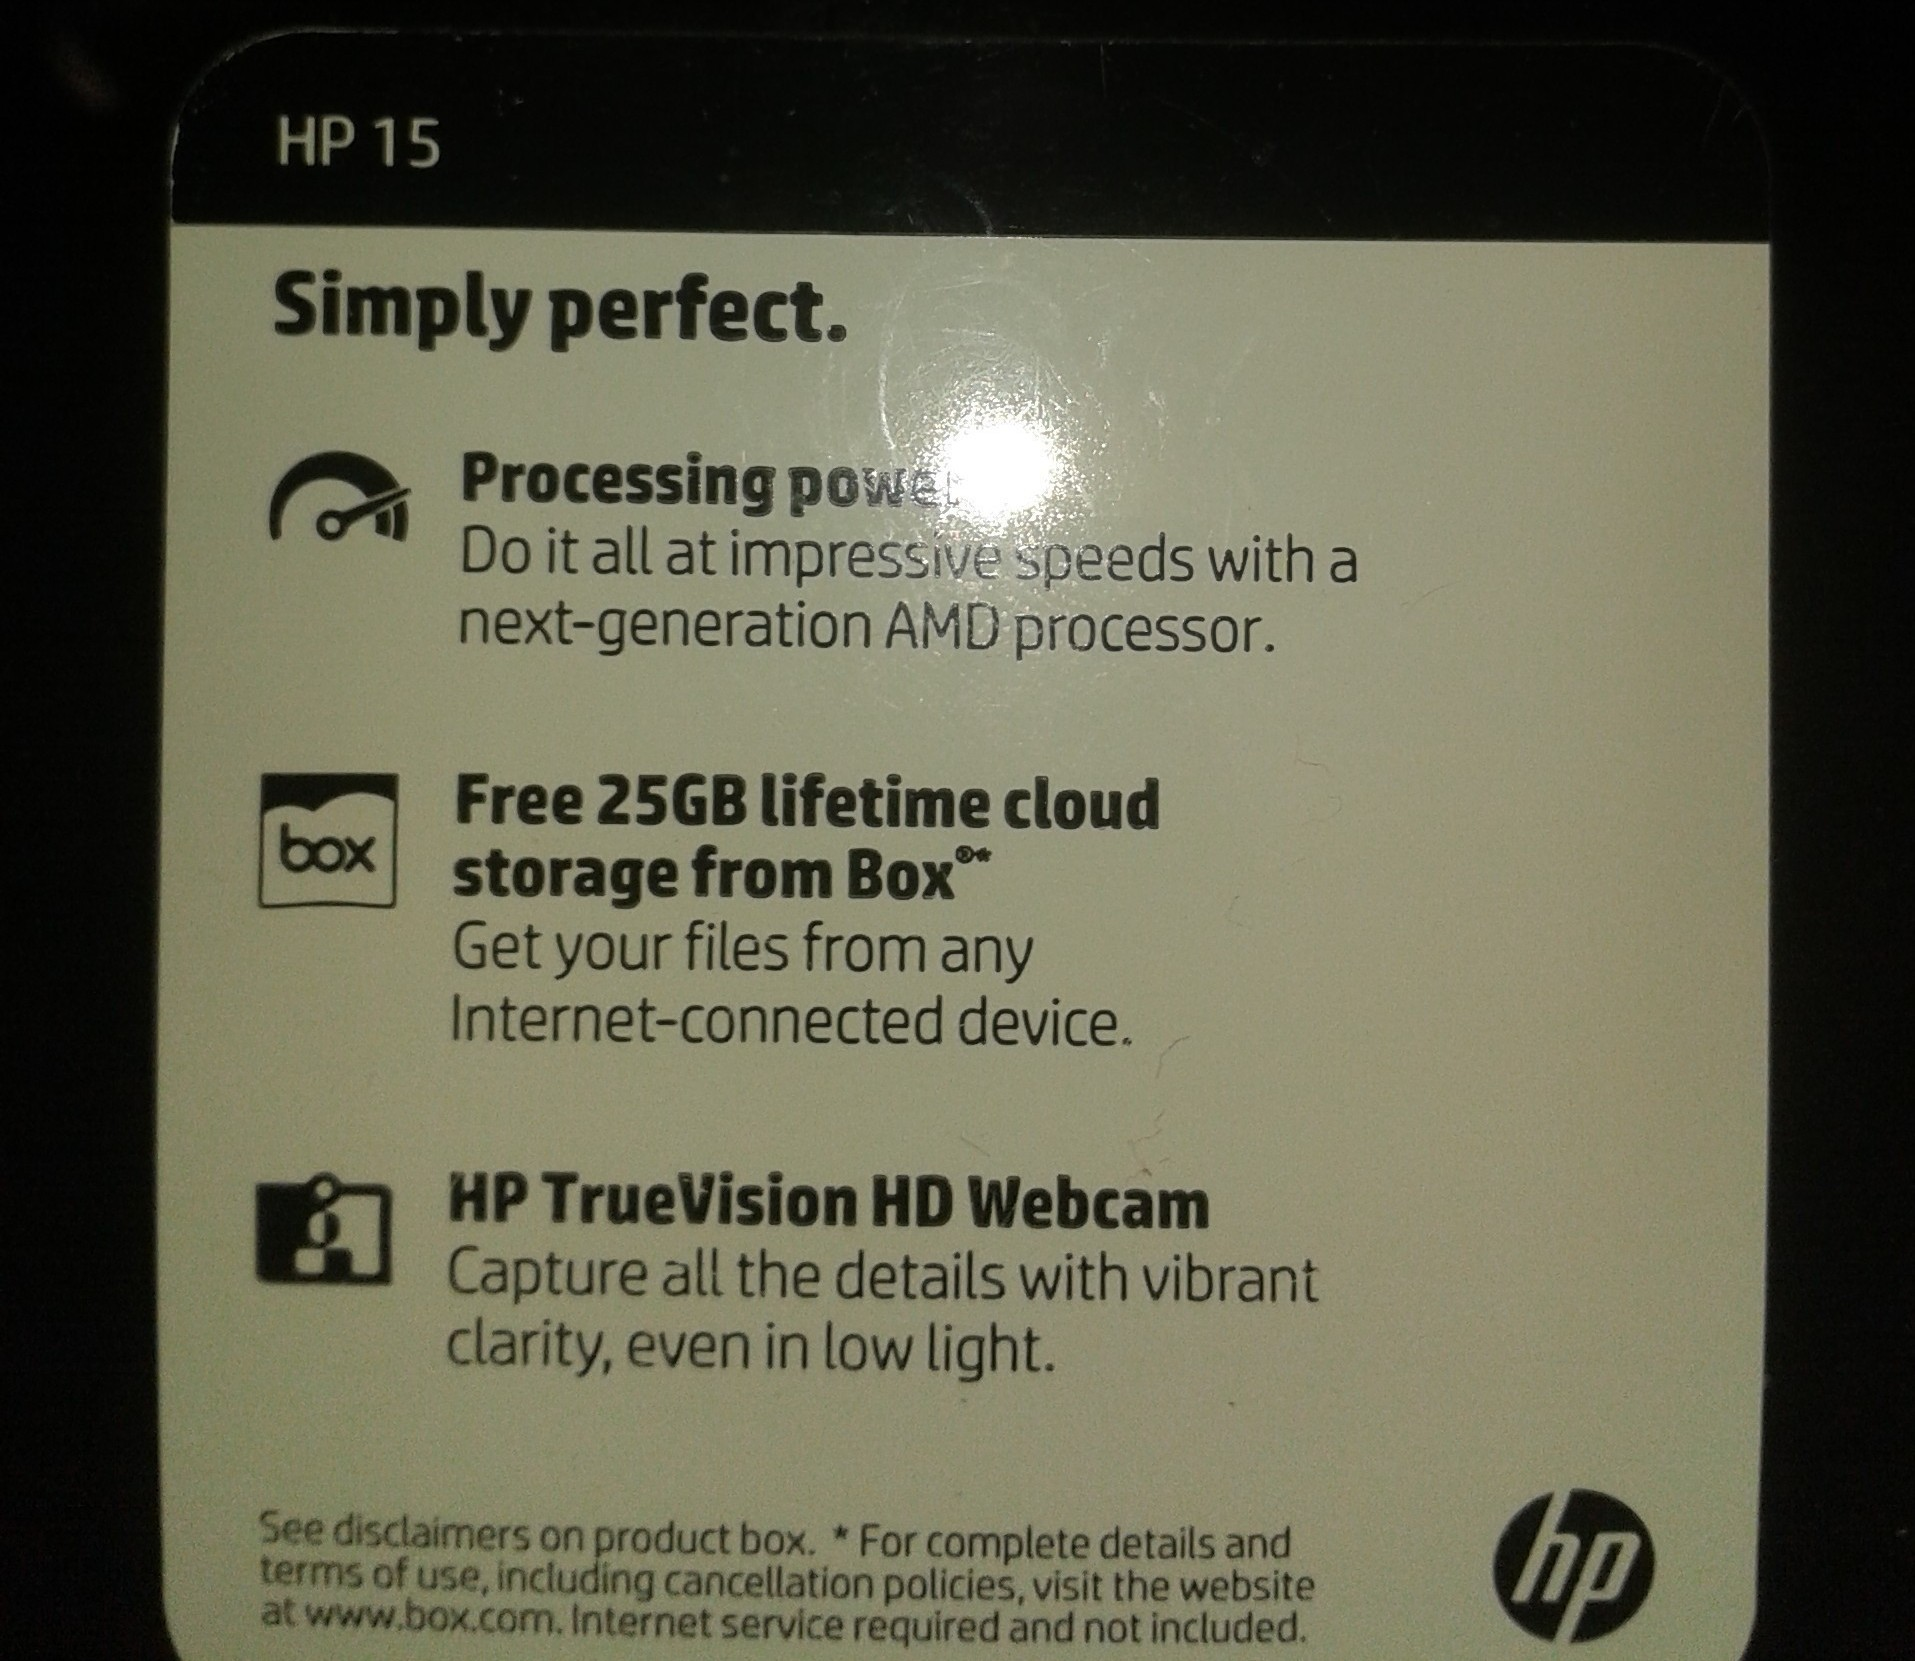
\includegraphics[scale=0.1]{./Resources/Teste-HP.jpg}
	\caption{Captura de imagem da etiqueta do computador HP para posterior descri��o}
	\label{Teste-HP}
	%\caption*{Source: some source}
\end{figure}



\newsavebox\MBox
\newenvironment{MinipageGreen}[1]
{\par\smallskip\begin{lrbox}{\MBox}\begin{minipage}{#1}}
		{\end{minipage}\end{lrbox}%
	\makebox(0,0){\put(0,0){%
			
\includegraphics[width=\wd\MBox,height=2\ht\MBox]{./Resources/green.jpg}
			}
	}%
	\usebox\MBox\par%
}
\newenvironment{MinipageRed}[1]
{\par\smallskip\begin{lrbox}{\MBox}\begin{minipage}{#1}}
		{\end{minipage}\end{lrbox}%
	\makebox(0,0){\put(0,0){%
			
\includegraphics[width=\wd\MBox,height=2\ht\MBox]{./Resources/red.jpg}
		}
	}%
	\usebox\MBox\par%
}

\newenvironment{MinipageYellow}[1]
{\par\smallskip\begin{lrbox}{\MBox}\begin{minipage}{#1}}
		{\end{minipage}\end{lrbox}%
	\makebox(0,0){\put(0,0){%
			
\includegraphics[width=\wd\MBox,height=2\ht\MBox]{./Resources/yellow.jpg}
		}
	}%
	\usebox\MBox\par%
}


\begin{figure}[H]
	
	\begin{subfigure}{.45\textwidth}
		
		
		\begin{MinipageGreen}{\textwidth} 
			
			\definecolor{green}{RGB}{140,255,26}
		%	\definecolor{red}{RGB}{255,71,71}
			
				\bf\color{white} nesta imagem est� escrito: \color{pink} shift shift ctrl \color{green} HP 15 Simply perfect. Processing power Do it all at impressive Speeds with a next-generation AMD processor. Free 25GB lifetime cloud \color{red}00X \color{green}storage from Box Get your files from any Internet-connected device. HP TrueVision HD Webcam Capture all the details with vibrant clarity, even in low light. See disclaimers on product box. For complete details and terms of use, including cancellation policies, visit the website at www.box.com, Internet service required and not included. \color{pink}alt
			
		\end{MinipageGreen}
		
		

		
		%\colorbox{dark-purple}{	
		
			%\parbox{.9\textwidth}{
				
				%\begin{verbatim}						
				
					%\color{white} nesta imagem est� escrito: \color{pink} shift shift ctrl \color{green} HP 15 Simply perfect. Processing power Do it all at impressive Speeds with a next-generation AMD processor. Free 25GB lifetime cloud \color{red}00X \color{green}storage from Box Get your files from any Internet-connected device. HP TrueVision HD Webcam Capture all the details with vibrant clarity, even in low light. See disclaimers on product box. For complete details and terms of use, including cancellation policies, visit the website at www.box.com, Internet service required and not included. \color{pink}alt
				
				%\end{verbatim}
				

		%	}			
		%}
		
	
		
		\captionof{figure}{}
		\label{RI}
	\end{subfigure}		
	\begin{subfigure}{.45\textwidth}
		
		\begin{MinipageYellow}{\textwidth}
			
			\definecolor{green}{RGB}{0,179,0}
			%\definecolor{red}{RGB}{255,71,71}
			
			\bf\color{white}nesta imagem est� escrito: \color{purple}shift ctrl \color{green}HP 15 Simply perfect. Processing \color{red}powe \color{green}Do it all at \color{red}impress peeds \color{green}with a next-generation AMD processor. Free 25GB lifetime cloud storage from Box Get your files from any Internet-connected device. HP True Vision HD Webcam Capture all the details with vibrant clarity, even in low light. See disclaimers on product box. For complete details and terms of use, including cancellation policies, visit the website at www.box.com Internet service required and not included. \color{purple}alt
			
		\end{MinipageYellow}
		
		%\fbox{
		
	%\colorbox{black}{	
			
			%\parbox{.9\textwidth}{			
				%\color{white}nesta imagem est� escrito: \color{purple}shift ctrl \color{green}HP 15 Simply perfect. Processing \color{red}powe \color{green}Do it all at \color{red}impress peeds \color{green}with a next-generation AMD processor. Free 25GB lifetime cloud storage from Box Get your files from any Internet-connected device. HP True Vision HD Webcam Capture all the details with vibrant clarity, even in low light. See disclaimers on product box. For complete details and terms of use, including cancellation policies, visit the website at www.box.com Internet service required and not included. \color{purple}alt 
			%}
			
	%}		
		%}
		\captionof{figure}{}
		\label{RII}
	\end{subfigure}		
	\begin{subfigure}{\textwidth}
	%\fbox{
	\vspace{1cm}
	

	\begin{MinipageRed}{\textwidth}
		
		\definecolor{red}{RGB}{255,128,128}
		
		\bf\color{white}nesta imagem est� escrito: \color{purple}shift \color{green}HP 15 Simply perfect. Processing \color{red}powR mpress \color{green}next-generation \color{red}ANAL pluce sul \color{green}Free 25GB lifetime \color{red}duud \color{green}storage from Box Get your files \color{red}Ton Jny \color{green}Internet connected \color{red}cevice \color{green}HP \color{red}Tru BVision HU Webo am Copture \color{green}the detais with vibrant \color{red}darity, \color{green}even \color{red}inluw lilli. box for compl-1 use inclue inteinetsarute resu ie: \color{purple}a
		
	\end{MinipageRed}
	
	%\colorbox{black}{
	
						
			%\parbox{\textwidth}{
				

								
				%\color{white}nesta imagem est� escrito: \color{purple}shift \color{green}HP 15 Simply perfect. Processing \color{red}powR mpress \color{green}next-generation \color{red}ANAL pluce sul \color{green}Free 25GB lifetime \color{red}duud \color{green}storage from Box Get your files \color{red}Ton Jny \color{green}Internet connected \color{red}cevice \color{green}HP \color{red}Tru BVision HU Webo am Copture \color{green}the detais with vibrant \color{red}darity, \color{green}even \color{red}inluw lilli. box for compl-1 use inclue inteinetsarute resu ie: \color{purple}a
			%}
			
			
			
			
			%}
		%}
		\captionof{figure}{}
		\label{RIII}
	\end{subfigure}	
	\caption{Resultado da extra��o apenas de texto sobre a imagem da Figura \ref{Teste-HP} com as resolu��es de (\protect\subref{RI}) 2560x1920, (\protect\subref{RII}) 1024x768 e (\protect\subref{RIII}) 480x360}
	\label{Resultado-HP}
\end{figure}


\definecolor{googleBlue}{rgb}{0.17,0.52,0.91} 
\newcolumntype{a}{>{\columncolor{googleBlue}\color{white}}l}

\begin{table}[H]
	
	\centering
	
	\caption{Tempos das fases da transcri��o de imagem sobre a etiqueta do computador HP, ilustrada pela Figura \ref{Teste-HP}}	
	
	\begin{tabular}{!{\color{googleBlue}\vrule} a  l  l  l !{\color{googleBlue}\vrule}}
		\arrayrulecolor{googleBlue} \hline
										
		Resultado					& \ref{RI} 	& \ref{RII}	& \ref{RIII}\\\hline
		Resolu��o             	& 2560x1920	    	& 1024x768          & 480x360  	       \\\hline
		
		Tempo de compress�o     		& 3667ms   		& 939ms		    	& 206ms  	       \\\hline
		Tempo de codifica��o    		& 570ms    	    & 69ms              & 66ms             \\\hline
		Tempo de transfer�ncia e processamento	& 103,849s	    & 17,871s   & 8,285s   	       \\\hline
		Tempo de reescrita              & 17ms		    & 97ms              & 4ms 	           \\\hline
		
		
	\end{tabular}
	\label{Estat-HP}	
\end{table}


Varias caracter�sticas importantes podem ser extra�das desses resultados. Primeiramente, a imagem possui um defeito causado pelo brilho intenso do flash concentrado num �nico ponto, no momento da captura e esse defeito afeta diretamente 3 palavras do texto. Essas palavras afetadas pelo brilho correspondem exatamente as malformadas, em vermelho, do resultado apresentado pela Figura \ref{RII}, erro esse que n�o ocorre com o apresentado pela Figura \ref{RI}. Isso permite a infer�ncia de que a redu��o da resolu��o pode ter tornado a OCR menos precisa e esse problema ter sido potencializado pelo brilho do flash ao ponto de distorcer completamente a grafia das palavras. 

� poss�vel que se o brilho refletido n�o tivesse sobreposto essas palavras, o resultado de \ref{RII} fosse muito semelhante ao de \ref{RI}. Essa hip�tese pode ser confirmada pela Tabela \ref{bestPracticesTable}, pois as dimens�es recomendadas pela Google para a detec��o de texto correspondem as da Figura \ref{RI}. Al�m disso, dimens�es inferiores reduzem a acur�cia do resultado, o que pode ser confirmado pela Figura \ref{RIII}, enquanto superiores aumentam o tempo de processamento e uso da largura de banda sem necessariamente promover melhora significativa da acur�cia\cite{bestPracticesGoogle}.


\begin{figure}[H]
	\centering
	
	\captionof{table}{Dimens�es de imagem recomendadas para cada caracter�stica buscada}
	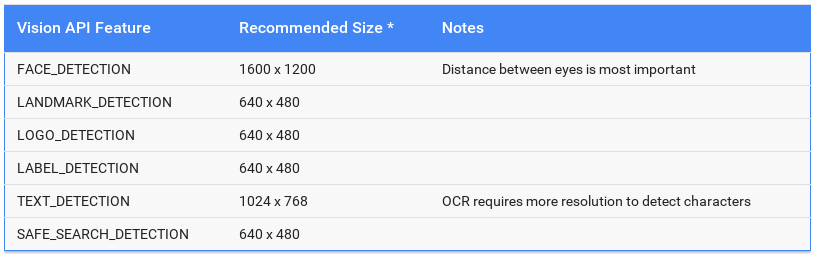
\includegraphics[scale=0.5]{./Resources/bestPractices.png}
	\caption*{Fonte: Google Cloud Platform\cite{bestPracticesGoogle}}

	\label{bestPracticesTable}
	
\end{figure}

\subsection{Teste para reconhecimento de texto girado}

Considerando o fato de que o usu�rio do aplicativo certamente n�o saber� de antem�o qual a posi��o do texto do qual deseja obter informa��es, � poss�vel ocorrer a captura de um texto de cabe�a para baixo. Ao se realizar os testes sobre textos com diferentes posi��es angulares, identificou-se que entre -90� e 90� n�o h� qualquer problema na extra��o de informa��o. Entretanto, acima desse limite, a aplica��o simplesmente n�o consegue mais identificar os caracteres corretamente. O resultado obtido pode ser visualizado pela Figura \ref{posicoes}

\begin{figure}[H]
	
	\begin{subfigure}{5cm}
		
		\centering
		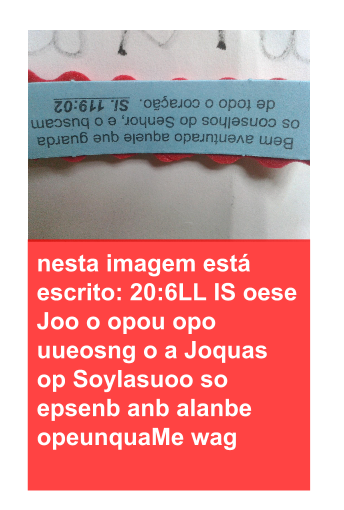
\includegraphics[scale=0.4]{./Resources/girado.png}
		\captionof{figure}{}
		\label{girado}
	
	\end{subfigure}		
	\begin{subfigure}{5cm}
		
		\centering
		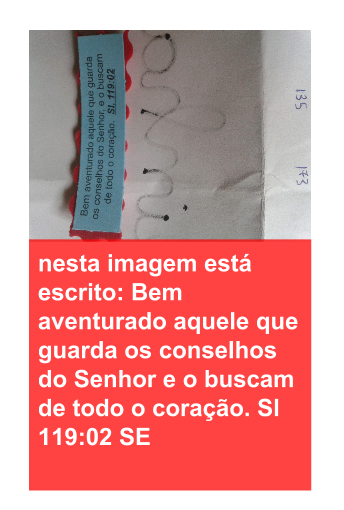
\includegraphics[scale=0.4]{./Resources/girado90.png}
		\captionof{figure}{}
		\label{girado90}
		
	\end{subfigure}		
	\begin{subfigure}{5cm}

		\centering
		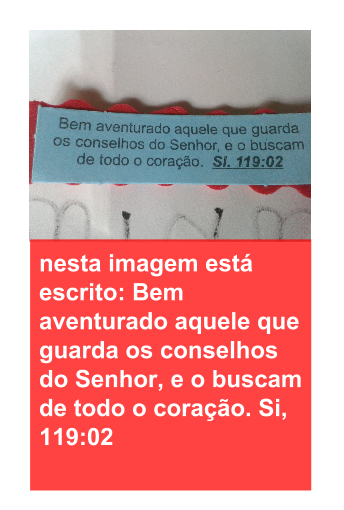
\includegraphics[scale=0.4]{./Resources/semgirar.png}
		\captionof{figure}{}
		\label{semgirar}
		
	\end{subfigure}	
	\caption{Extra��o apenas de texto de uma imagem sob tr�s diferentes posi��es. (\protect\subref{girado}) 180�, (\protect\subref{girado90}) 90� e (\protect\subref{semgirar}) 0�}
	\label{posicoes}
\end{figure} 

Apesar de esse resultado mostrar que h� uma limita��o na capacidade de API reconhecer caracteres, � poss�vel compreender a raz�o. Uma hip�tese � que o algoritmo apenas verifique que h� linhas horizontais de textos, e n�o considere a possibilidade de o texto estar virado em 180�. Ent�o, ele deve comparar o simbolo invertido com os de sua base de dados, e o que se encaixar melhor � considerado o correto. Ao analisar com mais cuidado a Figura \ref{girado}, pode-se perceber que apesar de o texto retornado n�o ter qualquer significado real, existe uma raz�o na forma��o de cada simbolo. H� uma consider�vel semelhan�a entre a letra "a" girada de 180� e a letra "e", entre "L" e "1", entre "w" e "m", e assim por diante. Quanto a Figura \ref{girado90}, praticamente n�o houve erros durante a OCR, mesmo apresentando um texto girado de 90�, assim como o teste apresentado  pela Figura \ref{semgirar}.


\subsection{Teste para reconhecimento de texto com letra cursiva}

Uma das possibilidades de utiliza��o do aplicativo seria a leitura de bilhetes escritos a m�o. Alguns testes foram realiza��o para se ter conhecimentos dos limites das capacidades da API, quanto a escrita a m�o, seja ela de forma ou cursiva. Os resultados mostraram que existe maior limita��o da API quanto a identifica��o de caracteres manuscritos, se comparada a de digitais. A Figura \ref{forma} apresenta o caso de um texto capturado com a mais alta resolu��o que o aplicativo oferece, de 2560x1920, e mesmo assim h� alguns erros de identifica��o. Por�m, como � poss�vel observar nas Figuras \ref{mao} e \ref{mao2}, os resultados s� ficam gravemente incorretos quando os textos s�o escritos em letra cursiva. Nesse cen�rio, o reconhecimento at� ocorre, mas de uma quantidade muito pequena do total de palavras, apresentando diversos erros, mesmo em tra�os largos e cor contrastante. Assim, a transcri��o de textos em letra cursiva se mostra, na pr�tica, imposs�vel pela aplica��o.


\begin{figure}[H]
	\centering	
	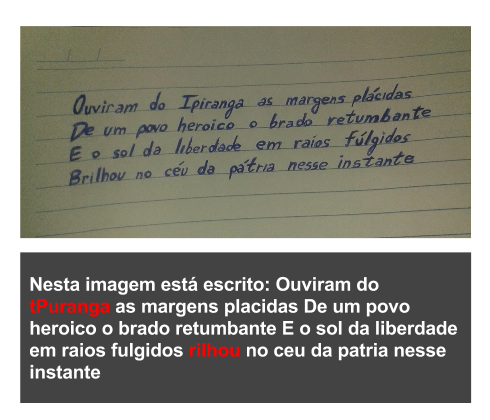
\includegraphics[scale=0.5]{./Resources/forma.png}
	\captionof{figure}{Resultado da extra��o de texto sobre imagem contendo escrita manual em letra de forma.}
	\label{forma}
	
\end{figure}

\begin{figure}[H]
	\centering	
	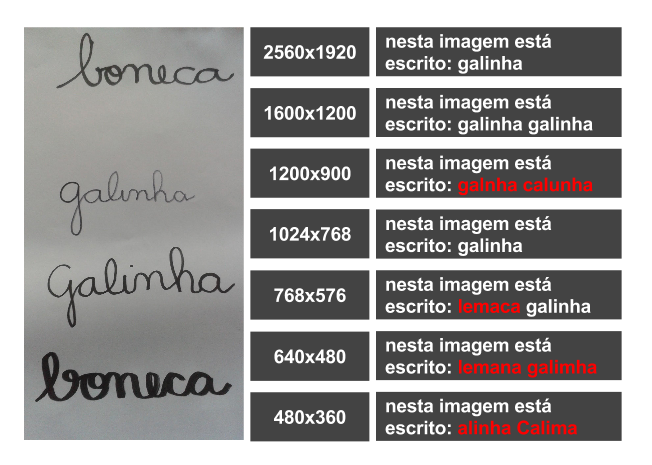
\includegraphics[scale=0.5]{./Resources/mao.png}
	\captionof{figure}{Resultados da extra��o de texto sobre imagem, em diferentes resolu��es, contendo palavras manuscristas em letra cursiva.}
	\label{mao}	
\end{figure}

\begin{figure}[H]
	\centering	
	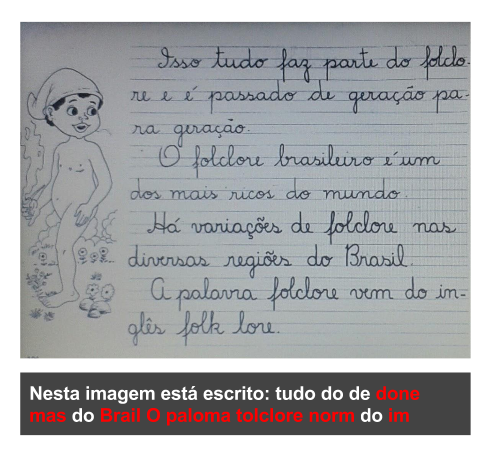
\includegraphics[scale=0.5]{./Resources/mao2.png}
	\captionof{figure}{Resultado da extra��o de texto sobre imagem contendo texto escrito em letra cursiva.}
	\label{mao2}	
\end{figure}


\subsection{Teste para rotula��o de elementos da cena}

Saber o que se passa tendo conhecimento do que h� ao redor � uma dos objetivos do projeto. Para saber o quais as limita��es da API na detec��o de objetos em imagens, foram realizados testes apontando a c�mera para os mais diversos objetos a fim de se avaliar sua performance nesse quesito. A Figura \ref{dogLabels} apresenta o resultado completo retornado pela extra��o de r�tulos da imagem de um cachorro. � poss�vel perceber que caracter�sticas como "Cachorro de brinquedo" e "Yorkshire Terrier" n�o s�o aplic�veis ao animal da foto. Como o aplicativo s� considera resultados com pontua��o acima de 80\%, r�tulos como esses, em vermelho, foram ignorados no resultado visualizado pelo usu�rio.

\iffalse
\begin{table}[H]
	
	\centering
	
	\caption{Tempos das fases da transcri��o de imagem sobre a etiqueta do computador HP, ilustrada pela Figura \ref{Teste-HP}}	
	
	\begin{tabular}{ll}
		
		Atributo				& Pontua��o \\
		Animal de estima��o    	& 95\% \\		
		Cachorro		        & 94\% \\
		Animal    	            & 93\% \\
		Mam�fero			    & 90\%      \\
		Cachorro de brinquedo   & 70\%	          \\
		Carn�voro      			& 68\%	          \\
		Yorkshire Terrier		& 52\%	          \\
	\end{tabular}
	\label{cachorro}	
\end{table}

\fi

\begin{figure}[H]
	\centering	
	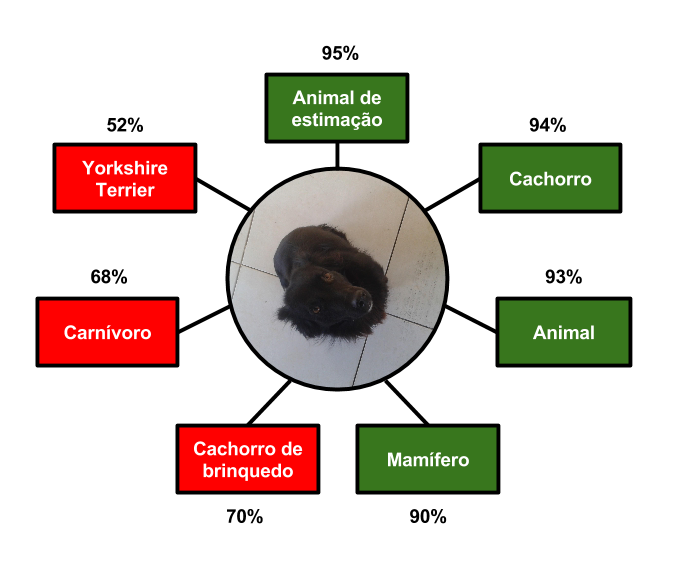
\includegraphics[scale=0.5]{./Resources/labels.png}
	\captionof{figure}{R�tulos extra�dos da imagem de um cachorro}
	\label{dogLabels}
	
\end{figure}

A escolha do valor m�nimo de pontos para que cada r�tulo fosse aceito foi puramente emp�rica. Apesar de ter resultado em boa descri��o para a imagem da Figura \ref{dogLabels}, o valor escolhido que elimina alguns resultados subaproveitou os r�tulos da imagem da Figura \ref{computerLabel}, descrevendo-a apenas como "Dispositivo", j� que "Laptop", palavra mais adequada, foi ignorada.

\begin{figure}[H]
	\centering	
	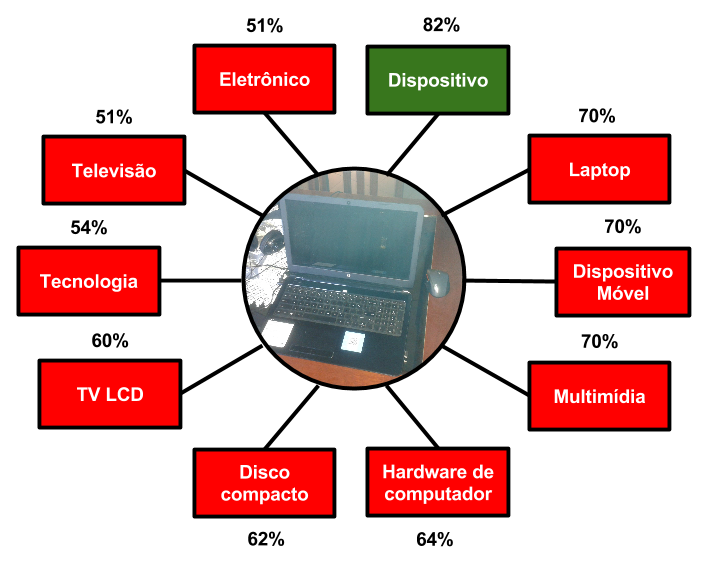
\includegraphics[scale=0.4]{./Resources/labelsComputer.png}
	\captionof{figure}{Primeira extra��o de r�tulos da imagem de um laptop}
	\label{computerLabel}
	
\end{figure}

A defini��o de um valor que simultaneamente seja capaz de descrever um elemento da cena e n�o sobrecarregue o usu�rio com informa��es, muitas vezes desnecess�rias, n�o � t�o simples, e uma descri��o curta e detalhada dificilmente ser� conseguida. No entanto, o resultado n�o depende apenas da defini��o desse valor, mas tamb�m da pr�pria imagem. A Figura \ref{computerLabel2} ilustra o mesmo laptop capturado novamente sob ilumina��o e posi��o diferentes. Nesse cen�rio, o resultado foi capaz de promover uma descri��o mais detalhada do objeto em cena.

\begin{figure}[H]
	\centering	
	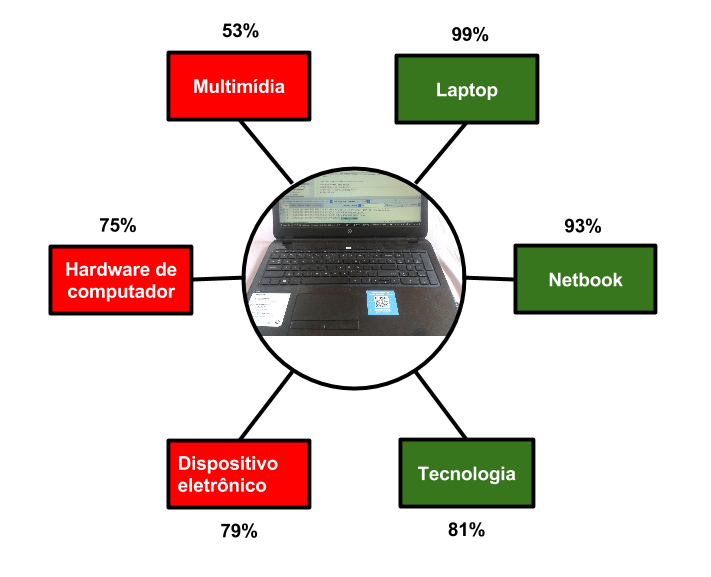
\includegraphics[scale=0.4]{./Resources/labelsComputer2.png}
	\captionof{figure}{Segunda extra��o de r�tulos da imagem de um laptop}
	\label{computerLabel2}
	
\end{figure}

Nos casos citados, independentemente de qual foi o crit�rio para ignorar alguns resultados, todos os r�tulos quase sempre tiveram rela��o com o objeto na imagem. Entretanto, em algumas situa��es a API falhou em identificar ao menos um r�tulo corretamente para a imagem capturada. A Figura \ref{cadeiraLabel} ilustra esse problema. Nela, foi capturada a imagem de uma cadeira, por�m al�m de n�o haver resultados acima do limite m�nimo de pontua��o, nenhum dos quatro r�tulos tem qualquer rela��o com a imagem.

\begin{figure}[H]
	\centering	
	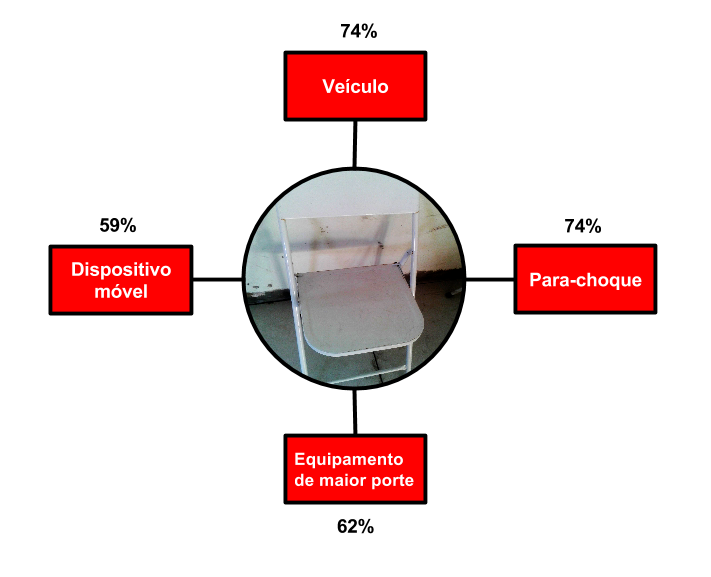
\includegraphics[scale=0.4]{./Resources/labelCadeira.png}
	\captionof{figure}{Extra��o de r�tulos da imagem de um cadeira}
	\label{cadeiraLabel}
	
\end{figure}

� poss�vel que a explica��o para esse resultado seja que o ambiente no qual a cadeira estava inserida tivesse afetado sua imagem capturada ao ponto de a API n�o ser capaz de identificar o que estava de fato em cena, e confundir o objeto com o para-choques de um ve�culo. Obviamente n�o � desej�vel que confus�es como essa ocorram, entretanto, esse � um fen�meno parecido com a "ilus�o de �ptica". Ao analisar a imagem, percebe-se que as faixas escuras entre a parede e o ch�o, atr�s da cadeira, somadas a sua estrutura em grades no meio podem ter sido avaliados como a parte frontal de um carro: Dois far�is pretos nas laterais, um cap� branco no topo e para-choques com grades na por��o centro-inferior.

\subsection{Teste para classifica��o de express�o facial}

Dentre as caracter�sticas que se pode obter de uma imagem, certamente a classifica��o de express�es faciais � a mais dif�cil de se obter. Como mostrou anteriormente a Tabela \ref{bestPracticesTable}, as dimens�es recomendadas para a detec��o de face � a maior dentre todas as outras caracter�sticas. Como apresentado na Se��o 4.1, o tempo de resposta cresce significativamente conforme a dimens�o da imagem aumenta. Isso significa que para se obter resultados corretos � necess�rio enviar a imagem com alta resolu��o e aguardar mais tempo. A Figura \ref{expressoes} apresenta o resultado obtido pela solicita��o do servi�o de detec��o de faces e extra��o de suas express�es faciais. As imagens foram tiradas diretamente pela c�mera do celular durante a execu��o do aplicativo a partir da exibi��o da tela do computador.

\begin{figure}[H]
	\centering	
	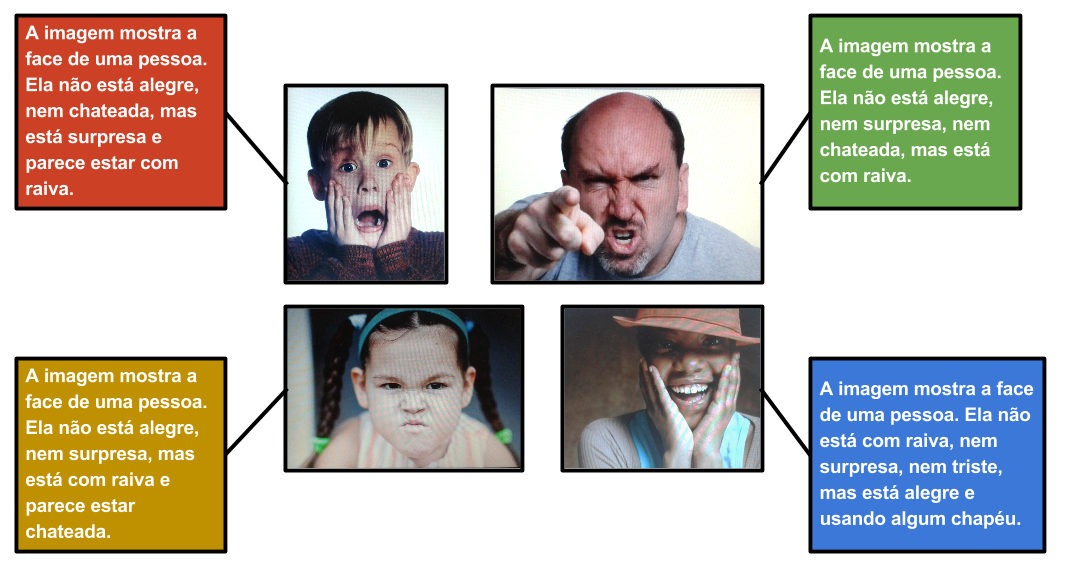
\includegraphics[scale=0.4]{./Resources/expressoes.png}
	\captionof{figure}{Express�es faciais detectadas em imagens de rosto}
	\label{expressoes}
	
\end{figure}

Apesar dos acertos nas descri��es das faces, os resultados n�o foram sempre corretos. Foi poss�vel perceber que a detec��o de express�es de raiva e tristeza dificilmente ocorriam, mesmo com o aumento da qualidade da imagem, ou com faces expressivas. A Figura \ref{triste} apresenta casos de falha com imagens de faces com express�es de tristeza. Os resultados variaram desde a n�o identifica��o da express�o evidente at� a incapacidade de encontrar a face.

\begin{figure}[H]
	\centering	
	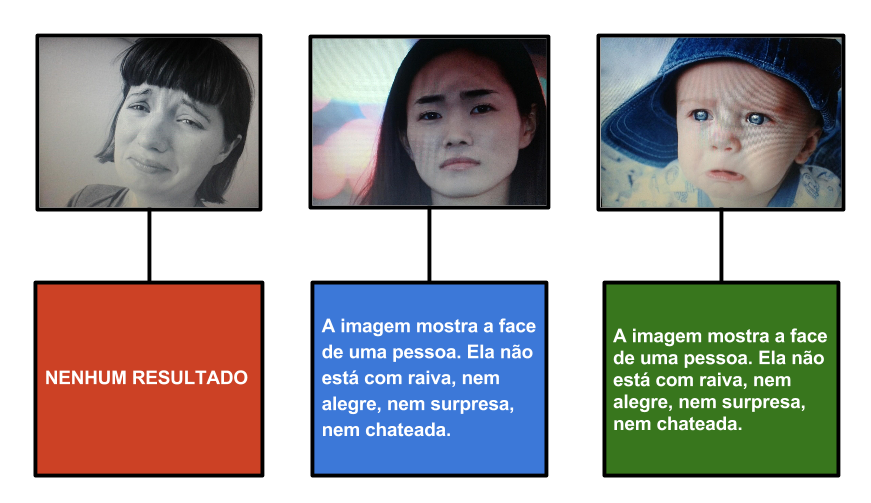
\includegraphics[scale=0.5]{./Resources/triste.png}
	\captionof{figure}{Express�es faciais de tristeza n�o detectadas em imagens de pessoas tristes}
	\label{triste}
	
\end{figure}




%\raggedright
\section{Detec��o de Obst�culos}

Na implementa��o da funcionalidade de detec��o de obst�culos, duas considera��es precisaram ser feitas. Primeiramente, para atender aos resultados esperados pelo usu�rio, o sensor de obst�culos deveria ser preciso o suficiente para garantir um deslocamento confi�vel. Al�m disso, procurou-se reduzir ao m�ximo o tamanho do circuito, para garantir sua usabilidade.

\subsection{Precis�o das medidas de dist�ncia}


Primeiramente, como havia a necessidade da cria��o de um circuito externo, o custo benef�cio foi analisado. Foi necess�ria a utiliza��o de um Ardu�no, um sensor de obst�culos, e um m�dulo de comunica��o. O Ardu�no em termos de capacidade de processamento se mostrou adequado  para a tarefa, que necessitava de baix�ssimo poder computacional: leitura de sinais e encaminhamento de dados. O sensor de obst�culos por ter uma abrang�ncia de 4 metros, mostrou ser aplic�vel para o prop�sito do projeto por fornecer margem suficiente de tempo de rea��o de um usu�rio caminhando [velocidade de caminhada, tempo de rea��o audi��o, tato, limite do sensor = 4m]. O m�dulo bluetooth utilizado tamb�m foi adequado, considerando que trata-se de dispositivos muito pr�ximos em comunica��o. 


\subsection{Usabilidade do dispositivo}

O segundo problema encontrado foi o tamanho dos elementos do circuito. Quanto menor, mais discreto e mais adapt�vel ao corpo ele se torna, o que n�o foi plenamente atingido [o circuito � um pouco maior que um smartphone].


\begin{figure}[H]
	\centering	
	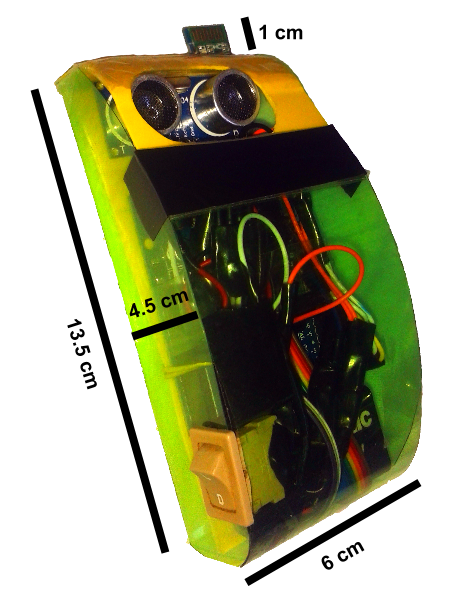
\includegraphics[scale=0.5]{./Resources/circuito.png}
	\captionof{figure}{Prot�tipo do circuito detector de obst�culos}
	\label{circuito}
	
\end{figure}


\section{Avalia��o de consumo do sistema}

O consumo de energia certamente � uma grande limitador na implementa��o de qualquer sistema. � importante portanto ter conhecimento da pot�ncia dissipada tanto pelo aplicativo executado no smartphone, quanto do circuito detector de obst�culos, formado pelo Ardu�no e demais m�dulos.

\subsection{Consumo no smartphone}
\subsection{Consumo no detector de obst�culos}

Para avaliar com maior precis�o o consumo de energia do circuito, durante 80 segundos foi medida a corrente consumida. Inicialmente, o circuito permaneceu ligado, por�m o aplicativo do smartphone estava desligado. Aos 30 segundos o aplicativo foi ligado e a fun��o de detec��o de obst�culos foi acionada. Nesse instante nota-se pela Figura \ref{ligaArduino} que houve uma queda na corrente. Isso ocorreu porque quando o m�dulo Bluetooth � alimentado, mas n�o est� conectado, ele fica constantemente enviando sinais para notificar sua presen�a. Quando uma conex�o � estabelecida, ele passa a enviar apenas os sinais de comunica��o, o que requer menos energia.

\begin{figure}[H]
	\centering	
	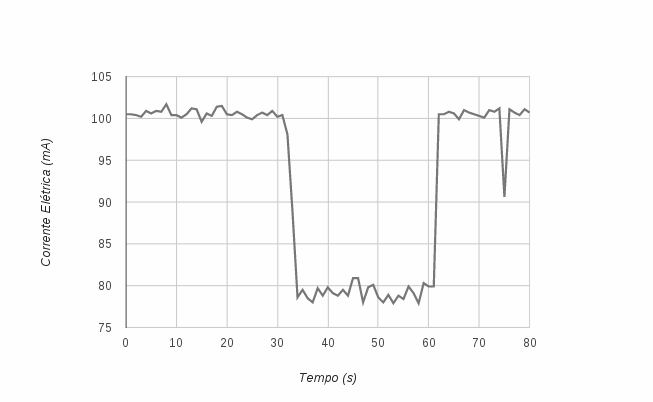
\includegraphics[scale=0.7]{./Resources/ligaArduino.png}
	\captionof{figure}{Corrente el�trica consumida pelo circuito antes, durante e ap�s a conex�o com o smartphone}
	\label{ligaArduino}
	
\end{figure}

Al�m de avaliar o consumo do circuito como um todo, avaliou-se tamb�m o quanto cada m�dulo conectado e devidamente ligado consome do total. Os m�dulos foram ativados de modo alternado a fim de se medir a corrente consumida individualmente, e para cada caso teste, o valor foi medido durante 25 segundos. O resultado pode ser visualizado pela Figura \ref{Modulos}, que mostra que a maior parte do consumo � resultado do funcionamento do Bluetooth.

\begin{figure}[H]
	\centering	
	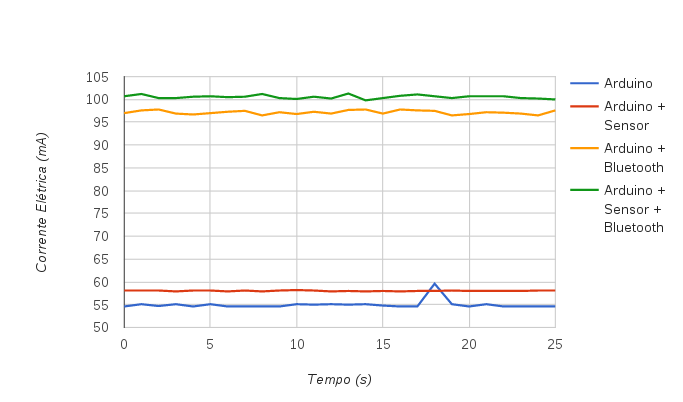
\includegraphics[scale=0.6]{./Resources/Modulos.png}
	\captionof{figure}{Corrente el�trica consumida pelo circuito discriminando o papel de cada m�dulo}
	\label{Modulos}
	
\end{figure}

A partir dos valores amostrados de corrente consumida pelo circuito, foi poss�vel calcular a corrente m�dia, o desvio padr�o e a pot�ncia m�dia, apresentados pela Tabela \ref{valoresMedios}. A pot�ncia $P$ foi calculada baseado no valor m�dio de corrente $I$ e na tens�o $V$ de alimenta��o de 9.6V, pela equa��o: \[ P = V x I \]

\definecolor{googleBlue}{rgb}{0.17,0.52,0.91} 
\newcolumntype{a}{>{\columncolor{googleBlue}\color{white}}l}

\begin{table}[H]
	
	\centering
	
	\caption{ Valores m�dios de corrente e pot�ncia consumidos pelos m�dulos do circuito}	
	
	\begin{tabular}{!{\color{googleBlue}\vrule} a  l  l  l l!{\color{googleBlue}\vrule}}
		\arrayrulecolor{googleBlue} \hline
		
		M�dulo				& Arduino 	& Sensor	& Bluetooth & Conjunto \\\hline
		Corrente M�dia(mA)  & 55		& 3.04      & 42.2       & 100.55\\\hline
		Desvio Padr�o (mA)	& 1			& 0.09		& 0.42      & 0.38  \\\hline
		Pot�ncia M�dia(mW)  & 529.5  	& 29.3    	& 406.2	    & 968.3 \\\hline		
		
	\end{tabular}
	\label{valoresMedios}	
\end{table}

De fato, o m�dulo Bluetooth consome pouco menos que o Ardu�no, representando quase a metade do consumo total. A Figura \ref{pizza} ilustra o resultado em percentuais de consumo.

\begin{figure}[H]
	\centering	
	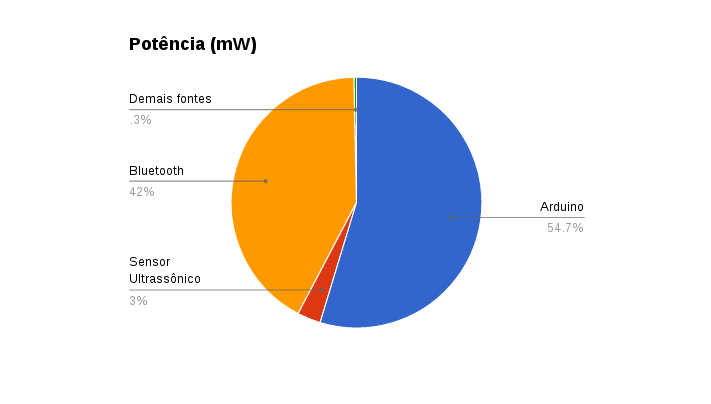
\includegraphics[scale=0.7]{./Resources/pizza.png}
	\captionof{figure}{Porcentagem de pot�ncia dissipada por cada m�dulo do circuito}
	\label{pizza}
	
\end{figure}






\chapter{Conclus�o ou Conclus�es}
\label{Conclusao}

Esse projeto teve como objetivo a aplica��o dos conhecimentos adquiridos durante a gradua��o a um problema real e que n�o possui tanto foco, que � o da acessibilidade de pessoas com defici�ncia visual. Foi poss�vel por meio desse trabalho aplicar alguns conceitos das seguintes disciplinas:

Programa��o Orientada a Objetos
Circuitos El�tricos
Laborat�rio de Circu�tos Eletr�nicos
Engenharia de software
An�lise de Desempenho de Sistemas Computacionais
An�lise e Projeto Orientados a Objeto
Microprocessadores e Aplica��es II





\section*{Trabalhos futuros}

Isso � para a Monografia Final de defesa.....












%%%%%%%%%%%%%%%%%%%%%%%%%%%%%%%%%%%%%% ADI��O DAS BIBLIOGRAFIAS %%%%%%%%%%%%%%%%%%%%%%%%%%%%%%%%%%%%%

\cleardoublepage
\setboolean{@twoside}{false}
\addcontentsline{toc}{chapter}{Refer�ncias}
\renewcommand{\bibname}{Refer�ncias}
	
\bibliographystyle{IEEEtran} % Define o estilo da bibliografia
\bibliography{./Content/References} % Faz referencia ao arquivo ref.bib


%%%%%%%%%%%%%%%%%%%%%%%%%%%%%%%%%%%%%%%%%% ADI��O DOS ANEXOS %%%%%%%%%%%%%%%%%%%%%%%%%%%%%%%%%%%%%%%%	
%\begin{appendices}
\appendix
\setboolean{@twoside}{true}
\cleardoublepage
\setboolean{@twoside}{false}

\chapter{Diagrama de classes do aplicativo Android}
\label{AndroidClassDiagram}
\begin{figure}[!hp]
	\centering	
	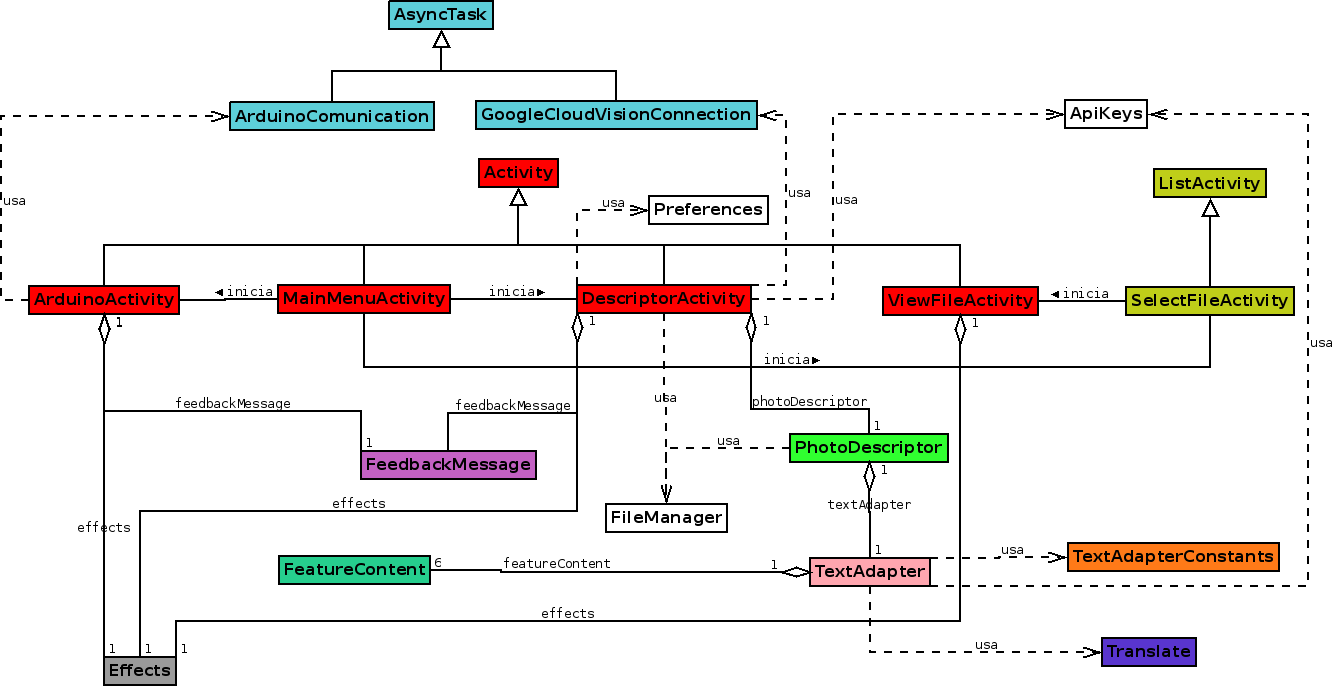
\includegraphics[angle=90,scale=0.46]{./Resources/AllClassesJustName.png}
	\captionof{figure}{Diagrama de classes do aplicativo baseado em android}
	\label{classCompact}
	
\end{figure}

\chapter{Diagrama de fluxo do aplicativo Android}
\label{AndroidFlowDiagram}
\begin{figure}[!hp]
	\centering	
	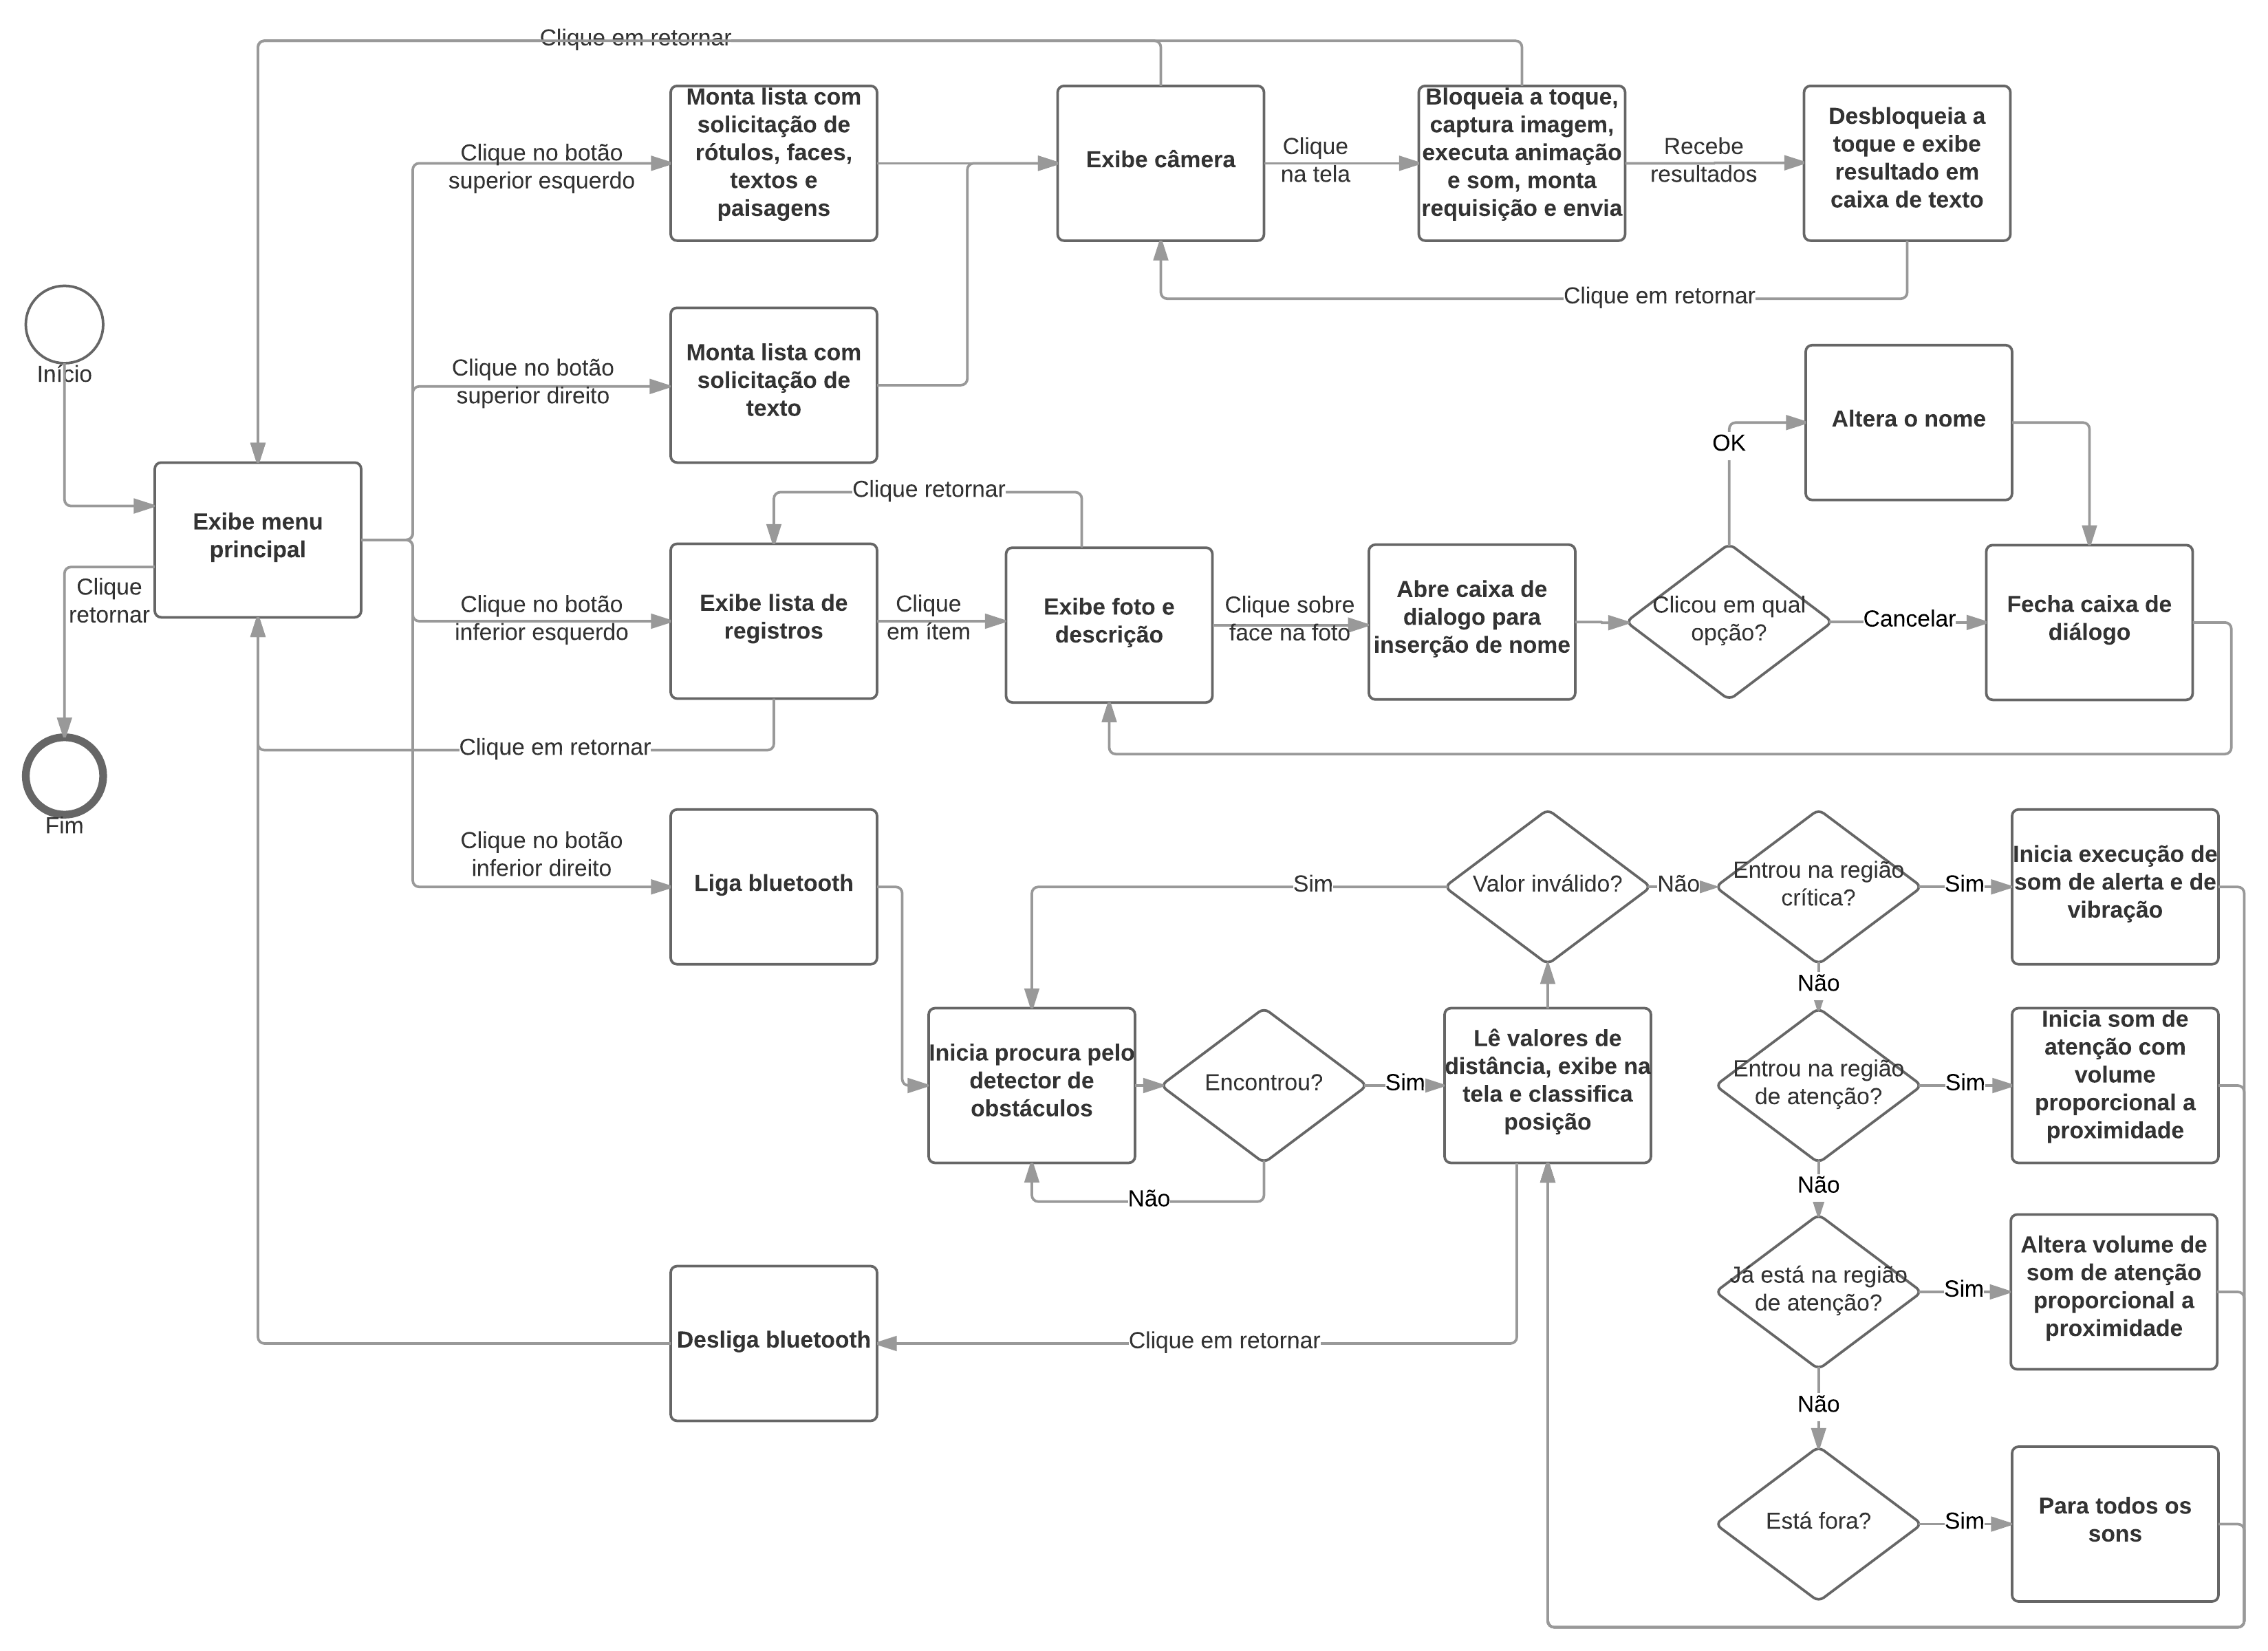
\includegraphics[angle=90,scale=0.18]{./Resources/diagramaEstados.png}
	\captionof{figure}{Diagrama de fluxo do aplicativo baseado em android}
	\label{flowCompact}
	
\end{figure}


\iffalse

\begin{center}
\textbf {\color{blue}{Dicas para a reda��o de uma boa monografia de TCC}}
\end{center}

Observe as diretrizes no site do Depto.
\begin{center}
\small{\textbf{http://www.sel.eesc.usp.br/informatica/graduacao/tcc/tcc\_-\_diretrizes\_EESC\_v\_2010.pdf}).}
\end{center}

Observe os elementos pr�-textuais neste documento....tem uma sequ�ncia a ser seguida (Capa, contracapa, Ficha catalogr�fica para a vers�o final, Listas de Figuras, Tabelas e S�mbolos/Abreviaturas).
- Resumo/abstract: texto em \underline{\textbf{um}} par�grafo apenas - deve conter \underline{tudo} resumidamente (introdu��o, m�todo(s), resultados e conclus�es), de tal forma que seja poss�vel compreender a proposta e o que foi alcan�ado;
	Palavras-chave: Logo abaixo do Resumo/Abstract.

\textbf{Cap�tulo 1} - Introdu��o: realmente introduz o leitor indicando quais s�o as dire��es do trabalho ? apresenta o tema e o objeto do trabalho e cont�m as Refer�ncias do Estado da arte (quem est� fazendo e em que n�vel os trabalhos da �rea est�o hoje);
- Justificativa/relev�ncia do trabalho: explana��o sobre porque o trabalho se justifica e quais os pontos de relev�ncia do mesmo;
- Objetivos: "somente" os objetivos ? podem ser gerais e/ou espec�ficos;
- Organiza��o do trabalho (o que tem em cada cap�tulo).
?	N�o h� necessidade de reproduzir (copiar) as obras que embasam o trabalho e sim colocar o suficiente para o entendimento do trabalho e citar as refer�ncias;

\textbf{Cap�tulo 2} - Embasamento Te�rico ou Fundamenta��o Te�rica: revis�o da literatura dos t�picos  que sustentam a ci�ncia e o conhecimento, relativos aos objetivos e o(s) m�todo(s) escolhido(s) para o desenvolvimento do trabalho;

\textbf{Cap�tulo 3} - Material e M�todos ou Desenvolvimento do Projeto: descri��o clara dos procedimentos e dos materiais adotados para o desenvolvimento do trabalho (sem resultados), incluindo sua adequa��o ao trabalho. 
Tem que responder �s perguntas: 
-est� com um tamanho adequado (proporcional) � monografia? 
-h� informa��o suficiente e clara sobre os materiais e sobre os m�todos  adotados?
N�o h� necessidade de reproduzir (copiar) as obras que embasam o trabalho e sim colocar o suficiente para o entendimento do trabalho e citar as refer�ncias;

\textbf{Cap�tulo 4} - Resultados/Discuss�es: aqui se mostra o que o trabalho permitiu produzir, e �s vezes o que pode ser comparado com outros trabalhos - aqui ficam claras se as propostas do trabalho s�o relevantes ou n�o, pois devem permitir a discuss�o do trabalho. 

Deve responder: Os resultados est�o claros em bom n�mero (nem muito nem pouco) que permitam avaliar realmente a proposta e o que foi produzido?

\textbf{Cap�tulo 5} - Conclus�es: "fecha" com os objetivos? (respondem aos objetivos?) - aqui � que "se vende o peixe"  pois ir�o valorizar (ou n�o) o trabalho realizado. Normalmente � uma parte do trabalho "um pouco desprezada", pois o autor j� est� "cansado....". Mas aqui � um ponto importante de medida se o trabalho tem ou n�o valor.
 
\textbf{Refer�ncias}: todas as refer�ncias {\color{red}{citadas no texto}}. Observar as Diretrizes, pois l� est�o os formatos corretos de cita��o.



\begin{center}	
\underline{Outras observa��es \textbf{IMPORTANTES} (\color{red}{leia isso com aten��o})}
\end{center}

NUNCA copie texto de outro autor sem a devida forma de cita��o (ver em diretrizes); a c�pia configura pl�gio! Com a Internet e/ou outras ferramentas dedicadas, � muito f�cil identificar se houve c�pia de texto.
Se voc� quiser verificar a porcentagem que seu texto apresenta de similaridade com outros na internet, baixe e rode o Copy Spider, por exemplo, ou consulte outros em  http://www.escritacientifica.sc.usp.br/anti-plagio/.
\begin{itemize}
\item [$\Rightarrow$] O tempo verbal a ser usado no texto, de forma geral, � o "PASSADO", pois o trabalho j� aconteceu;
\item [$\Rightarrow$] no texto, toda primeira vez que aparecer algum protocolo, procedimento, nome t�cnico, sigla, abreviatura, etc, al�m de explicar o que �, � necess�rio citar a refer�ncia. Exemplo: ...um girosc�pio (refer�ncia) � um tipo de sensor...
\item [$\Rightarrow$] figura que n�o � de sua autoria deve conter a fonte;
\item [$\Rightarrow$] capriche nas figuras (uma figura bem composta quase n�o precisa de texto para explic�-la);
\item [$\Rightarrow$] todas as figuras e  tabelas devem ser referenciadas no texto;
\item [$\Rightarrow$] procure manter a "Uniformidade de Nota��o" para o texto todo, ou seja, se denominou ou se referiu a algo ou algu�m de uma certa forma, mantenha essa forma para se referir durante todo o texto;
\item [$\Rightarrow$] n�o tenha medo de citar os trabalhos de outros autores (isso � imprescind�vel);
\item [$\Rightarrow$] evite muitas refer�ncias de sites, pois s�o vol�teis - procure boas refer�ncias nas bases consagradas como a IEEE, pois possuem artigos de �timo n�vel;
\item [$\Rightarrow$] N�O USE O WIKIPEDIA COMO REFER�NCIA;
\item [$\Rightarrow$] todas as palavras escritas em ingl�s (ou em outras l�nguas) devem estar em it�lico;
\item [$\Rightarrow$] cuidado com o uso de "atrav�s", que significa "atravessar" algo e n�o por meio de ;
\item [$\Rightarrow$] todas as obras citadas nas refer�ncias bibliogr�ficas devem estar citadas no texto;
\item [$\Rightarrow$] n�o use "satisfat�rio", "razo�vel" ou outra palavra que n�o seja precisa ou que n�o tenha sido definida a ordem de grandeza no projeto;
\item [$\Rightarrow$] c�digos de programas devem estar em Ap�ndices, pois servem para comprovar o desenvolvimento e facilitar a reprodu��o do trabalho;
\item [$\Rightarrow$] Anexos s�o materiais que n�o s�o de sua autoria, mas que s�o importantes e devem fazer parte da monografia para auxiliar e esclarecer o leitor;
\end{itemize} 

\fi

% % % % % % % % % % % % % % % % % % % % % % % % % % % % % % % % % % % % % % % % % % % % % % % % % % %

\setboolean{@twoside}{true}
\cleardoublepage
\setboolean{@twoside}{false}

\chapter{C�digos relevantes}
\label{relevantCode}

\definecolor{dkgreen}{rgb}{0,0.3,0}
\definecolor{gray}{rgb}{0.5,0.5,0.5}
\definecolor{mauve}{rgb}{0.58,0,0.82}
\definecolor{myorange}{rgb}{0.8,0.4,0}

\lstset{frame=tb,
	language=Java,
	aboveskip=3mm,
	belowskip=3mm,
	showstringspaces=false,
	columns=flexible,
	basicstyle={\small\ttfamily},
	numbers=left,
	numberstyle=\bfseries\tiny\color{gray},
	keywordstyle=\bfseries\color{blue},
	commentstyle=\color{gray},
	stringstyle=\bfseries\color{dkgreen},
	breaklines=true,
	breakatwhitespace=true,
	tabsize=3
}

\renewcommand{\lstlistingname}{C�digo}

Devido a dimens�o do projeto, a exposi��o de todo o c�digo utilizado como anexo dessa disserta��o mostrou-se invi�vel. Por essa raz�o, foram selecionados para serem fazerem parte desse documento apenas os c�digos considerados chave para o funcionamento do sistema. O c�digo completo pode ser encontrado em \url{https://github.com/guilherme-siqueira/projeto_final/tree/initialBranch/E-Eyes}. No C�digo \ref{textAdapter}, encontra-se a rotina respons�vel pela adapta��o textual da descri��o de uma imagem. Nela, considera-se primeiramente se h� alguma paisagem identificada, para ent�o avaliar poss�veis faces, r�tulos ou textos presentes. Caso n�o haja, o campo � ignorado, e apenas os campos mais internos, faces, r�tulos e textos, s�o considerados. Obter o n�mero de faces, em vez de apenas saber se h� ou n�o faces, permite que o texto possua concord�ncia verbal. No caso de n�o haver faces na imagem, considera-se apenas a poss�vel presen�a de r�tulos e textos. 

\begin{lstlisting}[caption=Rotina de constru��o do texto da descri��o da imagem,captionpos=b,label=textAdapter]
private void writeTextualDescription() {
	if (landmarkElement.getText() != null) {
		landmarkElement.translate();
		textualDescription = LANDMARK_INTRO + landmarkElement.getText() + ". ";
		if (nFaces == 1)
			textualDescription += FACE_INTRO + ONE_FACE + faceElement.getText();
		else if (nFaces == 2)
			textualDescription += FACE_INTRO + TWO_FACES + faceElement.getText();
		else if (nFaces > 2)
			textualDescription += FACE_INTRO + MORE_FACES_BEGINNING + nFaces + MORE_FACES_END + faceElement.getText();

		if (labelElement.getText() != null) {
			labelElement.translate();
			textualDescription += LABEL_INTRO + labelElement.getText();
		}

		if (textElement.getText() != null) {
			textualDescription += TEXT_INTRO + textElement.getText();
		}
	} 
	else if (nFaces != 0) {
		textualDescription = FACE_INTRO;
		if (nFaces == 1)
			textualDescription += ONE_FACE + faceElement.getText();
		else if (nFaces == 2)
			textualDescription += TWO_FACES + faceElement.getText();
		else if (nFaces > 2)
			textualDescription += MORE_FACES_BEGINNING + nFaces + MORE_FACES_END + faceElement.getText();

		if (labelElement.getText() != null) {
			labelElement.translate();
			textualDescription += LABEL_INTRO + labelElement.getText();
		}

		if (textElement.getText() != null) {
			textualDescription += TEXT_INTRO + textElement.getText();
		}
	} 
	else if (labelElement.getText() != null) {
		labelElement.translate();
		textualDescription = LABEL_INTRO + labelElement.getText();
		if (textElement.getText() != null) {
			textualDescription += TEXT_INTRO + textElement.getText();
		}
	} 
	else if (textElement.getText() != null) {
		textualDescription = TEXT_INTRO + textElement.getText();
	}
}
\end{lstlisting}



No c�digo \ref{google} encontra-se o m�todo respons�vel pelo envio da imagem e recebimento de sua descri��o. Primeiramente uma inst�ncia das funcionalidades da API da Google � criada e constru�da, por meio da classe Vision. Em seguida � criada uma inst�ncia de um objeto que permite m�ltiplas requisi��es de imagens, contendo a imagem capturada pelo aplicativo devidamente comprimida, o idioma para poss�veis textos escritos, e a lista de diferentes solicita��es requisitadas. Ent�o, um objeto de requisi��o de anota��o recebe todas as prefer�ncias criadas � executado, e o resultado retornado � recolhido para posterior convers�o em linguagem fluente, a partir da classe PhotoDescriptor. 

\begin{lstlisting}[caption=Rotina de conex�o e envio de dados para a Google Cloud Vision API,captionpos=b,label={google}]
protected boolean connect(){
	try {	
		HttpTransport httpTransport = AndroidHttp.newCompatibleTransport();
		JsonFactory jsonFactory = GsonFactory.getDefaultInstance();
		
		Vision.Builder builder = new Vision.Builder(httpTransport, jsonFactory, null);
		builder.setVisionRequestInitializer(new
		VisionRequestInitializer(CLOUD_VISION_API_KEY));
		Vision vision = builder.build();
		
		BatchAnnotateImagesRequest batchAnnotateImagesRequest =
		new BatchAnnotateImagesRequest();
		batchAnnotateImagesRequest.setRequests(new ArrayList<AnnotateImageRequest>() {{
		AnnotateImageRequest annotateImageRequest = new AnnotateImageRequest();
		
		Image base64EncodedImage = new Image();
		ByteArrayOutputStream byteArrayOutputStream = new ByteArrayOutputStream();		
		
		bitmap.compress(Bitmap.CompressFormat.JPEG, 90, byteArrayOutputStream);		
		byte[] imageBytes = byteArrayOutputStream.toByteArray();
		base64EncodedImage.encodeContent(imageBytes);
		annotateImageRequest.setImage(base64EncodedImage);
		
		ImageContext imageContext = new ImageContext();
		String [] languages = { "pt-BR" };
		imageContext.setLanguageHints(Arrays.asList(languages));
		annotateImageRequest.setImageContext(imageContext);		
		annotateImageRequest.setFeatures(requestsArrayList);		
		add(annotateImageRequest);
		}});
		
		Vision.Images.Annotate annotateRequest =
		vision.images().annotate(batchAnnotateImagesRequest);
		
		annotateRequest.setDisableGZipContent(true);
		Log.d(TAG, "created Cloud Vision request object, sending request");
		
		BatchAnnotateImagesResponse response = annotateRequest.execute();
		
		photoDescriptor.callTextAdaptation(response);
		
		return true;
	}
	catch (GoogleJsonResponseException e) {
		Log.d(TAG, "failed to make API request because " + e.getContent());
	}
	catch (IOException e) {
		Log.d(TAG, "failed to make API request because of other IOException " + e.getMessage());
	}
	return false;
}
\end{lstlisting}

J� o C�digo \ref{arduino} cont�m a rotina de captura dos sinais vindos do sensor de obst�culos HC-SR04, c�lculo da dist�ncia, e o envio para a porta serial, onde o m�dulo Bluetooth HC-05 � conectado. Primeiramente, define-se a taxa de transmiss�o da porta serial, o pino de sa�da de sinal para emiss�o de onda pelo sensor, e o pino de entrada, para recebimento do sinal correspondente ao tempo do eco refletido. 

No ciclo principal, monta-se a onda a ser emitida, com n�vel baixo de 2ms, e alto, de 10ms, respeitando as especifica��es m�nimas de utiliza��o do sensor, que podem ser encontradas no datasheet no Anexo \ref{SensorAnexo} . Em seguida l�-se o valor obtido de eco na porta de entrada, e a dist�ncia do obst�culo � calculada com base na equa��o $  S = V\times t $, em que $V$ representa a velocidade do som no ar em cent�metros por segundo, 0.034cm/s, e $t$ � a metade do tempo entre a emiss�o e a recep��o do sinal da onda, ou seja, o tempo entre a emiss�o da onda e o encontro com o obst�culo. Por fim, verifica-se se o valor lido n�o ultrapassou o limite de precis�o do sensor, de 4 metros, com o intuito de evitar valores pouco confi�veis, e a cada um segundo a rotina amostra o sinal e o envia para a porta serial, onde a entrada do bluetooth est� conectada. 



\lstset{frame=tb,
	aboveskip=3mm,
	belowskip=3mm,
	showstringspaces=false,
	columns=flexible,
	basicstyle={\small\ttfamily},
	numbers=left,
	numberstyle=\bfseries\tiny\color{gray},
	commentstyle=\color{gray},
	stringstyle=\bfseries\color{dkgreen},
	breaklines=true,
	breakatwhitespace=true,
	tabsize=3,
	keywordstyle=\bfseries\color{myorange},
	keywords={void, setup, loop, Serial, begin, delayMicroseconds, digitalWrite, pulseIn,if,println, pinMode, delay },
	rulecolor=\color{black},
	emphstyle=\bfseries\color{blue},
	emph={HIGH, INPUT, OUTPUT, LOW}
}

\begin{lstlisting}[caption=Rotina executada na placa Arduino,captionpos=b,label={arduino}]
//Define os pinos para o trigger e echo
#define pino_trigger 4
#define pino_echo 5

long duration;
int distance;

void setup()
{
	Serial.begin(9600);
	pinMode(pino_trigger, OUTPUT);
	pinMode(pino_echo, INPUT);
}

void loop()
{
	digitalWrite(pino_trigger, LOW);
	delayMicroseconds(2);
	// Sets the trigPin on HIGH state for 10 micro seconds
	digitalWrite(pino_trigger, HIGH);
	delayMicroseconds(10);
	digitalWrite(pino_trigger, LOW);
	// Reads the echoPin, returns the sound wave travel time in microseconds
	duration = pulseIn(pino_echo, HIGH);
	// Calculating the distance
	distance= duration*0.034/2;

	if(distance < 400)
	{
		Serial.println(distance);
		delay(1000);
	}
}
\end{lstlisting}


\iffalse
\begin{center}
\textbf {\color{blue}{Cuidados e orienta��es para a elabora��o da Apresenta��o do TCC}}
\end{center}


Todos os meus alunos me enviam a apresenta��o previamente, pois faz parte do procedimento que adoto para os TCCs.
Como tem-se at� 30 minutos para fazer a apresenta��o deve-se dimensionar a quantidade de slides para isso. Cada um tem seu "timming" com rela��o � quantidade de informa��o versus tempo dispon�vel para apresenta��o.
Os slides devem ser sempre muito mais visuais que textuais, ou seja, n�o se deve colocar frases e "ficar lendo" as mesmas. Os slides devem apresentar uma forma "clean" para que sirva apenas de guia para a apresenta��o do trabalho. 

N�o carregue de texto os slides...
Leia no site da El�trica (/Gradua��o/Trabalhos de Conclus�o de Curso - TCC) as DIRETRIZES GERAIS PARA ELABORA��O DO TRABALHO DE FORMATURA - TCC,
onde pode-se encontrar as Fichas de Avalia��o que s�o sugeridas pelo Depto, que n�o s�o necessariamente seguidas � risca pelos avaliadores, mas que servem de bom guia para os alunos entenderem como s�o feitas as avalia��es.
Tente n�o utilizar fundo escuro, pois escurece o ambiente e �s vezes n�o se consegue o visual esperado. Sempre que poss�vel teste antes no local da apresenta��o. 



% % % % % % % % % % % % % % % % % % % % % % % % % % % % % % % % % % % % % % % % % % % % % % % % % % %
\chapter{Monografia Parcial do TCC}
\label{Ap�ndice  Ap�ndice C}


\begin{center}
\textbf {\color{blue}{Cuidados e orienta��es para a composi��o da Monografia Parcial do TCC}}
\end{center}


Trata-se de uma Monografia completa, com todas as partes de uma Monografia final. 

Atente-se para as partes em {\color{red}{vermelho}}.

\begin{itemize}
\item Resumo
\item Introdu��o
\item Objetivos
\item Justificativas/Relev�ncia
\item Embasamento Te�rico (Fundamenta��o Te�rica-Revis�o Bibliogr�fica)
\item Material e m�todos ou Desenvolvimento do Projeto
\item {\color{red}{Resultados Preliminares}}
\item {\color{red}{Conclus�es Preliminares}}
\item {\color{red}{Sequ�ncia do trabalho (indicando poss�veis corre��es de rota do projeto)}}
\item {\color{red}{Cronograma Final (com corre��es se necess�rio)}}
\item Refer�ncias 
\item Ap�ndices
\item Anexos
\end{itemize} 

Sendo bem feito, ir� poupar esfor�o para a reda��o da monografia.

\fi

%\end{appendices}


\annex
\cleardoublepage

\addcontentsline{toc}{chapter}{Anexos}

\titleformat{\chapter}{\fontsize{16pt}{5mm}\selectfont\bfseries}{\hspace{1cm}Anexo \thechapter}{1em}{}

\iffalse
\chapter{Especifica��o t�cnica Ardu�no}
\label{ArduinoAnexo}

\setboolean{@twoside}{false}
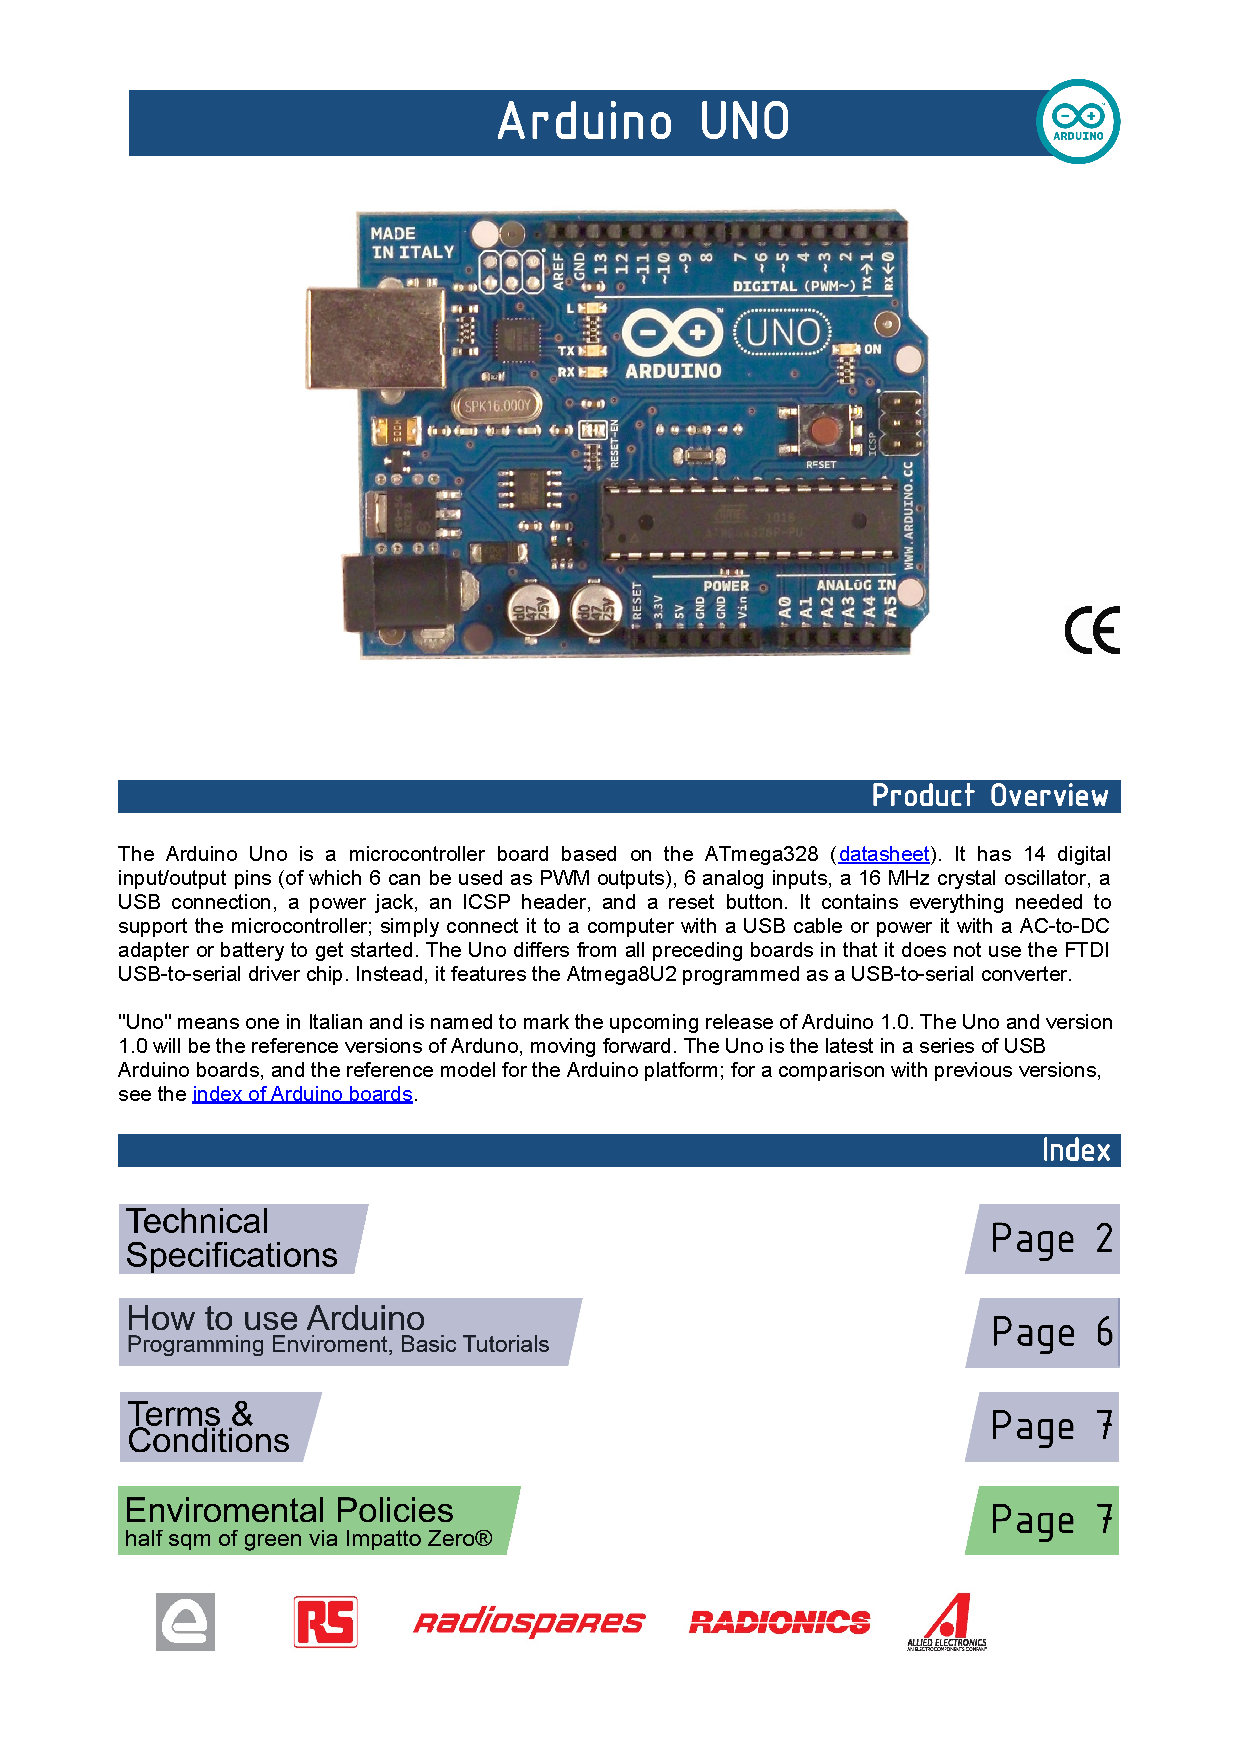
\includepdf[pages={1-2}]{Resources/ARDUINO-UNO.pdf}

\setboolean{@twoside}{true}
\cleardoublepage
\setboolean{@twoside}{false}

\fi
\chapter{Especifica��o t�cnica HC-05}
\label{Anexo}

\begin{figure}[H]
	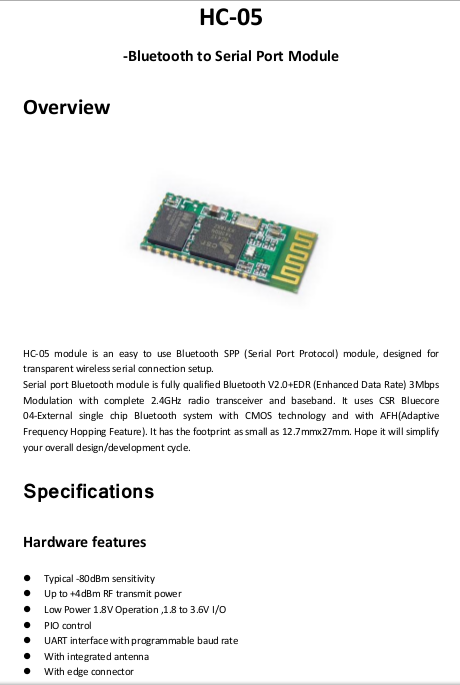
\includegraphics[scale=0.9]{./Resources/hcpageOne.png}
\end{figure}

\begin{figure}[H]
	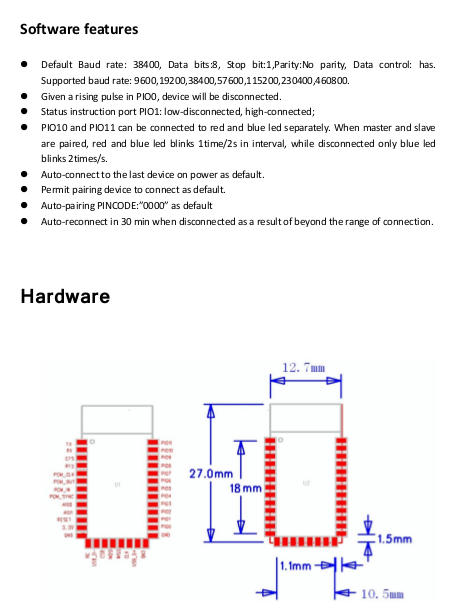
\includegraphics[scale=0.9]{./Resources/hcpageTwo.png}
\end{figure}

%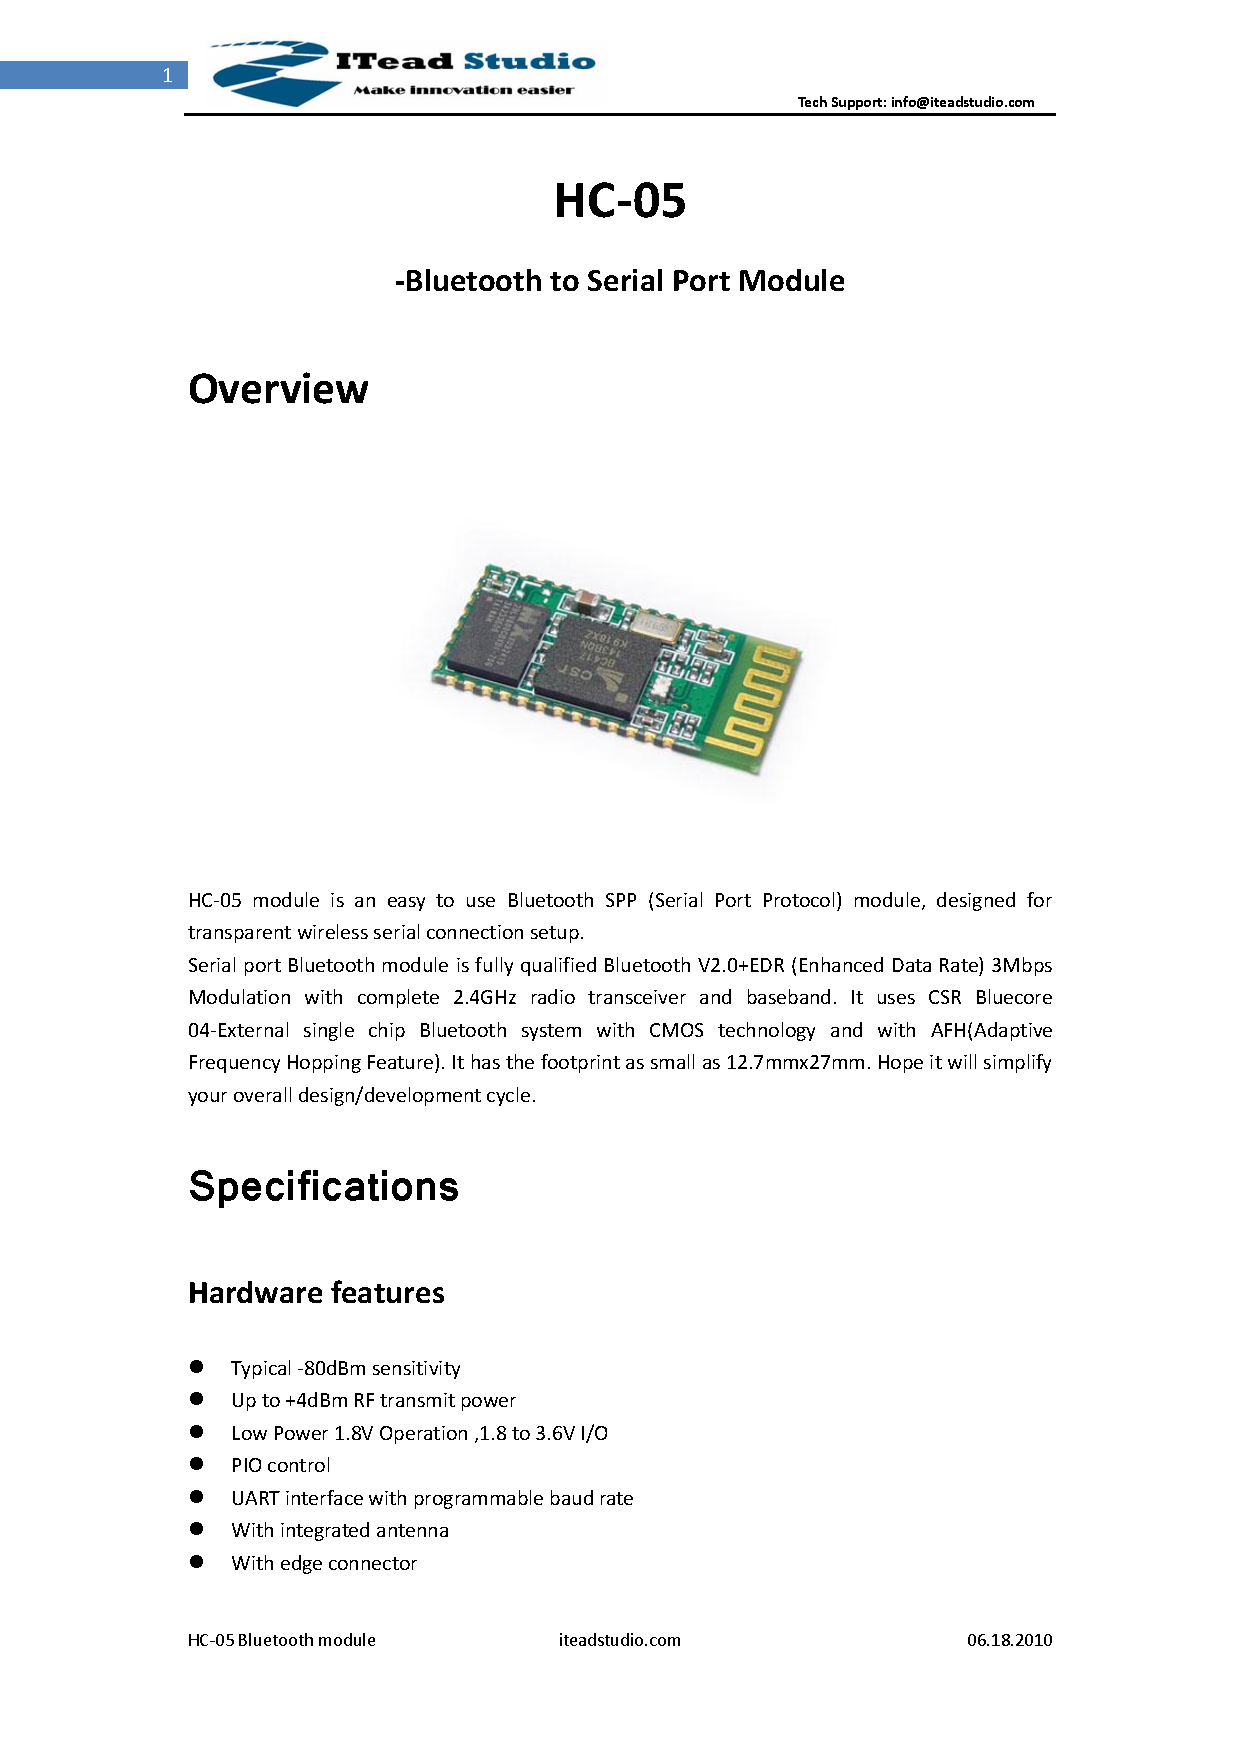
\includepdf[pages=1,pagecommand={\chapter{Datasheet HC-05} \thispagestyle{empty}}, offset=0cm -6cm fitpaper=true]{Resources/HC-05.pdf}

%\includepdf[pages=2,pagecommand={\thispagestyle{empty}}, fitpaper=true]{Resources/HC-05.pdf}

\iffalse
\includepdf[pages={2}]{Resources/HC-05.pdf}


\setboolean{@twoside}{true}
\cleardoublepage
\setboolean{@twoside}{false}
\fi

\chapter{Especifica��o t�cnica HC-SR04}
\label{SensorAnexo}

\begin{figure}[H]
	\includegraphics[scale=1]{./Resources/hcsrpageOne.png}
\end{figure}

\includepdf[pages={2,3}]{Resources/HCSR04.pdf}
%%%%%%%%%%%%%%%%%%%%%%%%%%%%%%%%%%%%%%% T�RMINO DO DOCUMENTO %%%%%%%%%%%%%%%%%%%%%%%%%%%%%%%%%%%%%%%%
\end{document}    
	